
\documentclass[12pt,twoside,openright]{book}

% Package imports for comprehensive document formatting
\usepackage[utf8]{inputenc}
\usepackage[T1]{fontenc}
\usepackage{lmodern}
\usepackage[english]{babel}
\usepackage{geometry}

\usepackage{amssymb}
\usepackage{graphicx}
\usepackage{xcolor}
\usepackage{listings}
\usepackage{booktabs}
\usepackage{tabularx}
\usepackage{longtable}
\usepackage{multirow}
\usepackage{hyperref}
\usepackage{tikz}
\usepackage{forest}
\usepackage{fancyhdr}
\usepackage{float}
\usepackage{tocloft}
\usepackage{enumitem}
\usepackage{subcaption}
\usepackage{float}
\usepackage{parskip}
\usepackage{titlesec}
\usepackage{microtype}
\usepackage{etoolbox}
\usepackage{pifont}
\usepackage{array}
\usepackage{amsmath,amssymb}
\usepackage{pdfpages}  % put in preamble
\usepackage[most]{tcolorbox}

\renewcommand{\arraystretch}{2}
\newcolumntype{L}{>{\raggedright\arraybackslash}X}
\usepackage{amsmath}
\usepackage{enumitem}
\tcbset{
    colback=blue!5!white,
    colframe=blue!75!black,
    title style={fill=blue!10!white},
    fonttitle=\bfseries
}

\usepackage{etoolbox}






% Define filled and empty star shortcuts
\newcommand{\starfull}{\ding{72}}   % filled star
% Define a star command
\newcommand{\starempty}{\ding{73}}  % empty star
% TikZ libraries for diagrams
\usetikzlibrary{shapes.geometric, arrows, positioning, fit, backgrounds, decorations.pathreplacing, matrix, shadows.blur, decorations.pathmorphing}

% Page geometry setup
\geometry{
    paper=a4paper,
    inner=1.5cm,
    outer=1.5cm,
    top=1in,
    bottom=1in,
    bindingoffset=0.5cm,
    headheight=14.5pt
}

% Hyperref configuration for PDF bookmarks and links
\hypersetup{
    colorlinks=true,
    linkcolor=blue,
    filecolor=magenta,      
    urlcolor=cyan,
    bookmarks=true,
    bookmarksopen=true,
    bookmarksopenlevel=2,
    pdfstartview=FitH,
    pdftitle={Multi-Agent Deal Discovery System: A Comprehensive Python Guide},
    pdfauthor={AI Assistant},
    pdfsubject={Python Programming, Machine Learning, Software Architecture},
    pdfkeywords={Python, Multi-Agent Systems, Machine Learning, Software Engineering, Deal Discovery}
}

% -----------------------------
% Syntax Colors
% -----------------------------
\definecolor{backcolour}{RGB}{245,245,245}      % light gray background
\definecolor{codegreen}{RGB}{28,172,0}         % comments
\definecolor{codegray}{RGB}{128,128,128}       % line numbers
\definecolor{codepurple}{RGB}{160,0,160}       % strings
\definecolor{keywordcolour}{RGB}{0,0,180}      % keywords
\definecolor{emerald}{RGB}{80,200,120}         % emerald color definition

% -----------------------------
% Listings Style
% -----------------------------
\lstdefinestyle{pythonstyle}{
    language=Python,
    basicstyle=\ttfamily\small,
    numbers=left,
    numberstyle=\tiny\color{codegray},
    frame=single,
    rulecolor=\color{gray!50},
    backgroundcolor=\color{backcolour},
    commentstyle=\color{codegreen},
    keywordstyle=\color{keywordcolour}\bfseries,
    stringstyle=\color{codepurple},
    breaklines=true,
    breakatwhitespace=true,
    keepspaces=true,
    showstringspaces=false,
    tabsize=4,
    columns=fullflexible,
    captionpos=b,
    xleftmargin=15pt,
    xrightmargin=15pt,
    aboveskip=10pt,
    belowskip=10pt
}

\lstset{style=pythonstyle}

% Custom command for checkmarks
% Enhanced chapter and section formatting
\titleformat{\chapter}[display]
{\normalfont\huge\bfseries\color{blue}}
{\chaptertitlename\ \thechapter}
{20pt}
{\Huge\color{black}}

\titleformat{\section}
{\normalfont\Large\bfseries\color{blue}}
{\thesection}
{1em}
{}

\titleformat{\subsection}
{\normalfont\large\bfseries\color{blue!70}}
{\thesubsection}
{1em}
{}

\titleformat{\paragraph}[runin]
{\normalfont\normalsize\bfseries}
{\theparagraph}
{1em}
{}[.]

% Enhanced headers and footers
\pagestyle{fancy}
\fancyhf{}
\fancyhead[LE,RO]{\thepage}
\fancyhead[LO]{\nouppercase{\rightmark}}
\fancyhead[RE]{\nouppercase{\leftmark}}
\renewcommand{\headrulewidth}{0.4pt}




% Table of contents customization
\renewcommand{\cftchapfont}{\bfseries\large}
\renewcommand{\cftsecfont}{\normalsize}
\renewcommand{\cftsubsecfont}{\small}
\setlength{\cftbeforechapskip}{12pt}
\setlength{\cftbeforesecskip}{6pt}
\setlength{\cftbeforesubsecskip}{3pt}

% Enhanced list formatting
\setlist[itemize,1]{label=\textbullet, leftmargin=20pt}
\setlist[itemize,2]{label=\textendash, leftmargin=15pt}
\setlist[enumerate,1]{label=\arabic*., leftmargin=20pt}
\setlist[enumerate,2]{label=\alph*), leftmargin=15pt}

% Document metadata
\title{
    \Huge\textbf{Multi-Agent Deal Discovery System}\\[0.5cm]
    \Large\textit{A Comprehensive Python Programming Guide}\\[0.3cm]
    \large From Architecture to Implementation:\\
    Machine Learning, Web Scraping, and System Design
}

\author{
    \large AI Assistant\\[0.2cm]
    \small Generated Documentation for Advanced Python Development\\[0.1cm]
    \small September 29, 2025
}

\date{\today}

% Begin document
\begin{document}

%% Title page with enhanced formatting
\frontmatter
% --- Enhanced Colorful Title Page ---
\begin{titlepage}
    \thispagestyle{empty} % No headers or footers on the cover

 % --- Define a lighter, vibrant color palette ---
\definecolor{coverdeepspace}{RGB}{50, 60, 90}    % Lighter dark blue
\definecolor{coverneonglow}{RGB}{100, 240, 210}  % Lighter bright teal/cyan
\definecolor{coverpurple}{RGB}{160, 120, 240}    % Lighter vibrant purple
\definecolor{covermagenta}{RGB}{240, 120, 190}   % Lighter bright magenta
\definecolor{covertext}{RGB}{245, 250, 255}      % Almost white for text


    % Use TikZ for a full-page, multi-layered design
    \begin{tikzpicture}[remember picture, overlay]
        % --- Layer 1: The Background ---
        % A deep space gradient from top-left to bottom-right
        \fill[shade, left color=coverdeepspace, right color=black]
            (current page.south west) rectangle (current page.north east);

        % --- Layer 2: Abstract "Digital Network" Graphics ---
        % Faint, glowing lines to suggest connections and data flow
        \foreach \i in {1,...,20}{
            \draw[coverneonglow, line width=0.4pt, opacity=0.08, decoration={random steps, segment length=5mm, amplitude=0.2mm}, decorate]
                ($(current page.west) + (0, \i*1.5)$) -- ($(current page.east) + (0, \i*1.8-15)$);
            \draw[coverpurple, line width=0.4pt, opacity=0.08, decoration={random steps, segment length=3mm, amplitude=0.3mm}, decorate]
                ($(current page.north) + (\i*1.5-15, 0)$) -- ($(current page.south) + (\i*1.2-12, 0)$);
        }

        % --- Layer 3: Central Graphical Element (Abstract Agent Network) ---
        \begin{scope}[
            transform canvas={yshift=-2cm, scale=1.1},
            every node/.style={
                circle,
                fill=coverneonglow,
                inner sep=1.5pt,
                opacity=1,
                blur shadow={shadow blur steps=8, shadow opacity=60}
            }
        ]
            \node (c) at (current page.center) {};
            \node (n1) at ($(c) + (120:3cm)$) {};
            \node (n2) at ($(c) + (240:3cm)$) {};
            \node (n3) at ($(c) + (0:3cm)$) {};
            \node (n4) at ($(c) + (60:5cm)$) {};
            \node (n5) at ($(c) + (180:5cm)$) {};
            \node (n6) at ($(c) + (-60:5cm)$) {};
            
            \draw[coverneonglow!70, line width=1pt, opacity=0.4] (n1)--(n2)--(n3)--(n1);
            \draw[coverpurple!80, line width=0.7pt, opacity=0.3] (n4)--(n1)--(n5)--(n2)--(n6)--(n3)--(n4);
            \draw[covermagenta!70, line width=0.5pt, opacity=0.3] (c)--(n1) (c)--(n2) (c)--(n3);

             % --- Brain image on the left (override circular style) ---
    
        \end{scope}
        \node[anchor=east, fill=none, draw=none, inner sep=0pt, opacity=1] 
        (brain) at ($(c) + (8cm,11.5cm)$) {\includegraphics[width=6cm]{brain.png}};
        \node[anchor=east, fill=none, draw=none, inner sep=0pt, opacity=1] 
        (brain1) at ($(c) + (-3cm,11.6cm)$) {\includegraphics[width=6cm]{brain2.png}};
        \node[anchor=east, fill=none, draw=none, inner sep=0pt, opacity=1] 
        (brain1) at ($(c) + (2.7cm,11.6cm)$) {\includegraphics[width=6cm]{brain3.png}};
        

        % --- Layer 4: Content positioning and styling ---

        % % Main Title with a subtle glow effect
        % \node[anchor=center, align=center] at ($(current page.center) + (0, 8cm)$) {
        %     \fontsize{32}{36}\selectfont\bfseries
        %     \color{coverneonglow!30!black!80} % Shadow color
        %     Multi-Agent Deal Discovery System
        % };
        \node[anchor=center, align=center] at ($(current page.center) + (-0.7pt, 8cm+0.7pt)$) {
            \fontsize{28}{30}\selectfont\bfseries
            \color{covertext} % Main text color
            Multi-Agent Deal Discovery System
        };
        
        % Subtitle
        \node[anchor=center, align=center] at ($(current page.center) + (0, 5.5cm)$) {
            \Large\itshape\color{coverneonglow}
            A Comprehensive Python Programming Guide
        };

        % Decorative rule
        \draw[coverpurple, line width=0.5pt, opacity=0.7] ($(current page.center) + (-8cm, 4cm)$) -- ($(current page.center) + (8cm, 4cm)$);
        
        % Tertiary title
        \node[anchor=center, align=center] at ($(current page.center) + (0, 3cm)$) {
            \large\color{covertext!90}
            From Architecture to Implementation:\\[0.4cm]
            \color{coverpurple!90!white}Machine Learning, \color{covermagenta!90!white}Web Scraping, \color{covertext!90}and \color{coverneonglow}System Design
        };
        
       \node[
        anchor=south, 
        text width=0.9\textwidth, 
        align=center, 
        inner sep=20pt,            % more padding     % optional rounded background   % subtle background behind text
        text=covertext,
    ] at ($(current page.south) + (0, 2cm)$) {
        {\LARGE \textbf{SIJAN PAUDEL}}\\[0.4cm]
        {\LARGE Generated Technical Documentation}\\[0.3cm]
    };
    \end{tikzpicture}
\end{titlepage}
% --- End of Title Page ---


% Table of Contents with enhanced formatting
\newpage
\tableofcontents
\newpage
\listoffigures
\newpage
\listoftables
\newpage
\lstlistoflistings


% Preface
\chapter*{Preface}
\addcontentsline{toc}{chapter}{Preface}

This comprehensive guide provides an in-depth analysis of a sophisticated multi-agent deal discovery system implemented in Python. The system demonstrates advanced software engineering principles, modern Python programming techniques, and practical machine learning integration.

\section*{What You'll Learn}

This documentation covers:

\begin{itemize}
    \item \textbf{Advanced Python Programming}: Object-oriented design, inheritance patterns, composition, and modern Python idioms
    \item \textbf{System Architecture}: Multi-agent design patterns, component interaction, and scalable system design
    \item \textbf{Machine Learning Integration}: Ensemble methods, LLM APIs, vector databases, and traditional ML models
    \item \textbf{Web Technologies}: RSS parsing, HTML scraping, HTTP clients, and API integration
    \item \textbf{Production Practices}: Error handling, configuration management, logging, and performance optimization
\end{itemize}

\section*{How to Use This Guide}

The guide is structured in seven comprehensive parts:

\begin{enumerate}
    \item \textbf{System Overview}: High-level architecture and component relationships
    \item \textbf{File Analysis}: Detailed examination of each Python file
    \item \textbf{Class Hierarchy}: Object-oriented design patterns and inheritance
    \item \textbf{Function Breakdown}: Method-by-method analysis with execution details
    \item \textbf{Python Concepts}: Advanced language features with practical examples
    \item \textbf{Agent Interactions}: Workflow analysis and sequence diagrams
    \item \textbf{Summary \& Knowledge}: Complete system recap and learning outcomes
\end{enumerate}

Each part builds upon the previous sections while remaining accessible for focused study of specific topics.

\section*{Prerequisites}

Readers should have:
\begin{itemize}
    \item Basic Python programming knowledge
    \item Understanding of object-oriented programming concepts
    \item Familiarity with common Python libraries (requests, json, etc.)
    \item Basic knowledge of machine learning concepts (optional but helpful)
\end{itemize}

\section*{Code Conventions}

Throughout this guide:
\begin{itemize}
    \item Code snippets are syntax-highlighted for readability



Important concepts are marked with ratings (\starfull\starempty\starempty\starempty\starempty\ to \starfull\starfull\starfull\starfull\starfull)

    \item Cross-references link related concepts across chapters
    \item Diagrams illustrate complex system interactions
\end{itemize}

\mainmatter

% Part 1: System Overview and Architecture
\chapter{LLM Cheat Sheet}

\section{Handling Imports from Parent Folders in Python and Jupyter}

When a Python script or Jupyter Notebook is located in a subfolder, modules in a parent folder may not be automatically discoverable by Python. The following methods illustrate how to properly import them.

\subsection{Using \_\_file\_\_ in Python Scripts}

For scripts executed directly, \_\_file\_\_ contains the path of the script. Use it to construct the parent folder path:

\begin{tcolorbox}[colback=red!5,colframe=red!70!black,title=Python Script: Using \_\_file\_\_]
\begin{verbatim}
import sys
import os

# Add parent folder to Python path
sys.path.append(os.path.abspath(os.path.join(os.path.dirname(__file__), '..')))

# Import module from parent folder
from LLMengineering import key_utils
\end{verbatim}
\end{tcolorbox}

\textbf{Explanation:}
\begin{itemize}
    \item \texttt{os.path.dirname(\_\_file\_\_)}: folder of the current script.
    \item \texttt{os.path.join(..., '..')}: go one level up.
    \item \texttt{os.path.abspath(...)}: get absolute path.
    \item \texttt{sys.path.append(...)}: add this path to Python's module search paths.
\end{itemize}

\subsubsection{Using \texttt{os.getcwd()} in Jupyter Notebooks}

In Jupyter, \_\_file\_\_ is not defined. Use the current working directory instead:

\begin{tcolorbox}[colback=gray!5, colframe=gray!80!black, title=Jupyter Notebook: Using os.getcwd()]
\begin{verbatim}
import sys
import os

# Add parent folder of current working directory
sys.path.append(os.path.abspath(os.path.join(os.getcwd(), '..')))

# Import module from parent folder
from key_utils import some_function
\end{verbatim}
\end{tcolorbox}

\textbf{Notes:}
\begin{itemize}
    \item \texttt{os.getcwd()}: returns the current working directory of the notebook.
    \item \texttt{..} moves one level up; \texttt{../..} moves two levels up.
    \item This approach is portable for notebooks without relying on \_\_file\_\_.
\end{itemize}

\subsubsection{Using Absolute Paths (Less Portable)}

\begin{tcolorbox}[colback=gray!5, colframe=gray!80!black, title=Absolute Path Approach]
\begin{verbatim}
import sys
sys.path.append("/run/media/sijanpaudel/New Volume/New folder/LLMengineering")

from key_utils import some_function
\end{verbatim}
\end{tcolorbox}


\textbf{Caution:} This works immediately but is hard-coded. If the project moves, the path must be updated.

\subsubsection{Recommended Long-Term Approach}

1. Add an empty \_\_init\_\_.py file in the parent folder (e.g., \texttt{LLMengineering/}) to make it a package.
2. Use relative or absolute imports within scripts:

\begin{tcolorbox}[colback=gray!5, colframe=gray!80!black, title=Long-Term Package Approach]
    \begin{verbatim}
    from LLMengineering import key_utils
    \end{verbatim}
\end{tcolorbox}

This makes imports clean, portable, and avoids repeated \texttt{sys.path.append} hacks.



\newpage
\section{Comparing LLMs -- The Basics (1)}
\begin{tabularx}{\textwidth}{|>{\hsize=0.3\hsize}L|>{\hsize=0.7\hsize}L|}
\hline
\textbf{Feature} & \textbf{Description / Notes} \\
\hline
Open-source or Closed & Whether the model’s weights, architecture, and training code are publicly available. Examples: GPT-4 (closed), LLaMA 2 (open). \\
\hline
Release Date \& Knowledge Cut-off & The date the model was released and the latest point in time the training data covers. Important for up-to-date responses. \\
\hline
Parameters & Number of trainable weights in the model (e.g., billions of parameters). Determines model capacity. \\
\hline
Training Tokens & Amount of text data used during training, usually in billions of tokens. More tokens generally improve performance. \\
\hline
Context Length & Maximum input length (in tokens) the model can handle in a single prompt. Longer context allows better understanding of large inputs. \\
\hline
\end{tabularx}

\vspace{1em}

\section{Comparing LLMs -- The Basics (2)}

\begin{tabularx}{\textwidth}{|>{\hsize=0.3\hsize}L|>{\hsize=0.7\hsize}L|}
\hline
\textbf{Feature} & \textbf{Description / Notes} \\
\hline
Inference Cost & Computational resources required to generate output (GPU, CPU usage). \\
\hline
API Charge / Subscription / Runtime Compute & How much it costs to access the model through a cloud service. \\
\hline
Training Cost & Cost to pretrain the model, including compute, electricity, and infrastructure. \\
\hline
Build Cost & Cost to fine-tune, deploy, or customize the model. \\
\hline
Time to Market & How quickly you can deploy and use the model in production. \\
\hline
Rate Limits & Restrictions on API usage, e.g., calls per minute or per day. \\
\hline
Speed \& Latency & How fast the model responds, depends on model size, hardware, and context length. \\
\hline
License & Terms for use, redistribution, and commercial deployment. Some open-source licenses restrict commercial use. \\
\hline
\end{tabularx}

\vspace{1em}

\section{Chinchilla Scaling Law}

\textbf{Key Principle:} Number of model parameters should scale roughly proportional to the number of training tokens.

\textbf{Implications:}
\begin{itemize}
    \item Increasing model size without enough data leads to plateaued or degraded performance.
    \item Having lots of training data with a small model underperforms; parameters must scale up.
\end{itemize}

\textbf{Rule of Thumb:} Let $N$ = model parameters, $D$ = training tokens. For optimal training:
\[
N \propto D
\]

\textbf{Example:}
\begin{itemize}
    \item Doubling model parameters $\rightarrow$ need roughly double the training tokens.
    \item Insufficient tokens $\rightarrow$ diminishing returns.
\end{itemize}

\textbf{Additional Notes:}
\begin{itemize}
    \item Smaller, well-trained models can outperform larger, undertrained ones.
    \item Helps determine compute-efficient configurations for new LLMs.
\end{itemize}

\vspace{1em}

\section{Common LLM Benchmarks}
\begin{tabularx}{\textwidth}{|>{\hsize=0.2\hsize}X|>{\hsize=0.3\hsize}X|>{\hsize=0.5\hsize}X|}
\hline
\textbf{Benchmark} & \textbf{Focus / Task} & \textbf{Description} \\
\hline
MMLU & Knowledge across multiple subjects & Assess general knowledge and reasoning; used to compare models like GPT-3, Chinchilla, and Gopher. \\
\hline
BIG-bench & Broad suite of diverse reasoning tasks & Tests reasoning, factual knowledge, ethics, math, code; hundreds of tasks evaluating beyond narrow QA. \\
\hline
HellaSwag & Commonsense reasoning & Multiple-choice questions for everyday situations; measures ability to predict plausible outcomes. \\
\hline
TruthfulQA & Factual accuracy / truthfulness & QA tasks designed to detect hallucinations; evaluates honesty of LLM answers. \\
\hline
WinoGrande / Winograd Schema Challenge & Pronoun resolution / coreference & Tests commonsense reasoning and context understanding; resolves ambiguous references. \\
\hline
ARC & Science and reasoning & Multiple-choice science questions; evaluates problem-solving and reasoning in STEM. \\
\hline
HumanEval & Coding and code generation & Tests Python programming ability; measures functional correctness of generated code. \\
\hline
\end{tabularx}

\vspace{1em}

\section{Specific Benchmarks}

\begin{tabularx}{\textwidth}{|>{\hsize=0.2\hsize}X|>{\hsize=0.3\hsize}X|>{\hsize=0.5\hsize}X|}
\hline
\textbf{Benchmark} & \textbf{What’s Being Evaluated} & \textbf{Description} \\
\hline
ELO & Model ranking / performance consistency & Evaluates models via pairwise comparisons; creates a relative ranking of LLMs across multiple tasks. \\
\hline
HumanEval & Code generation / functional correctness & Tests an LLM’s ability to write Python functions that pass unit tests; measures coding logic and correctness. \\
\hline
Multipl-E & Multimodal reasoning & Evaluates LLMs on tasks combining text and images (or multiple modalities); measures reasoning and comprehension across modalities. \\
\hline
\end{tabularx}

\vspace{1em}

\section{Limitations of Benchmarks}

\begin{tabularx}{\textwidth}{|>{\hsize=0.6\hsize}L|>{\hsize=1.4\hsize}L|}
\hline
\textbf{Limitation} & \textbf{Explanation} \\
\hline
Narrow focus & Many benchmarks test only specific skills (e.g., coding, factual QA, commonsense), not overall intelligence or adaptability. \\
\hline
Static datasets & Benchmarks are fixed in time, so models trained after the cut-off may have an unfair advantage or miss newer knowledge. \\
\hline
Lack of real-world context & Benchmarks often use idealized tasks, not messy, ambiguous, or multi-step real-world scenarios. \\
\hline
Gaming / overfitting & Models can be fine-tuned or prompted to specifically excel on benchmark tasks without improving general capabilities. \\
\hline
Limited multimodality & Most benchmarks focus on text-only tasks; few measure image, audio, or multimodal reasoning. \\
\hline
Subjectivity & Some benchmarks (e.g., ethics, creativity, hallucination detection) are hard to score objectively. \\
\hline
Compute bias & Larger models may perform better mainly due to size, not reasoning ability, skewing benchmark results. \\
\hline
Hard to measure nuanced reasoning & Benchmarks mostly measure surface correctness; they often cannot capture multi-step reasoning, context-dependent judgment, creativity, or reasoning accuracy vs. fluency. \\
\hline
\end{tabularx}

\section{Advanced Benchmarks for Large Language Models}

\begin{tabularx}{\textwidth}{|>{\hsize=0.2\hsize}X|>{\hsize=0.3\hsize}X|>{\hsize=0.5\hsize}X|}
\hline
\textbf{Benchmark} & \textbf{Focus / Task} & \textbf{Description / Meaning} \\
\hline
GPQA & Graduate-level question answering & Evaluates performance on graduate-level tests with 448 expert questions. Non-PhD humans score only 34\% even with web access. Measures LLM ability to handle highly specialized knowledge. \\
\hline
BBHard & Future capabilities & Includes 204 tasks previously thought beyond LLM capabilities. Designed to test reasoning, logic, and generalization at a next-level difficulty. \\
\hline
Math Lv 5 & High-school math competition problems & Measures model’s ability to solve advanced math problems requiring multi-step reasoning and problem-solving skills. Useful for chain-of-thought evaluation. \\
\hline
IFEval & Instruction following & Tests the model’s ability to follow complex instructions, e.g., “write more than 400 words” and “mention AI at least 3 times.” Evaluates comprehension and compliance with nuanced prompts. \\
\hline
MuSR & Multistep soft reasoning & Assesses logical deduction and multi-step reasoning. Example: analyzing a 1,000-word story and identifying “who has means, motive, and opportunity.” Tests reasoning beyond surface facts. \\
\hline
MMLU-PRO & Harder MMLU version & Advanced, cleaned-up version of MMLU with questions having 10 possible answers instead of 4. Evaluates deeper knowledge, multi-choice reasoning, and generalization. \\
\hline
\end{tabularx}

\vspace{1em}
\textbf{Notes:}
\begin{itemize}
    \item These benchmarks are considered “next-level” because they test advanced reasoning, multi-step logic, and high-level knowledge.  
    \item Useful for evaluating models that go beyond standard QA, commonsense reasoning, or basic coding tasks.  
    \item Many of these benchmarks also measure compliance with complex instructions and reasoning under uncertainty. 
\end{itemize}


\begin{tabularx}{\textwidth}{|>{\hsize=0.15\hsize}X|>{\hsize=0.85\hsize}X|}
\hline
\textbf{Benchmark} & \textbf{Purpose / Examples} \\
\hline
GPQA & Specialized knowledge, expert-level Q\&A, academic reasoning, physics, chemistry, biology expertise.  \newline
\textbf{Examples:} Explain the biochemical steps of glycolysis; Describe Newton’s laws with practical applications; Explain photosynthesis in detail. \\
\hline
BBHard & Advanced reasoning, logic, generalization in challenging scenarios.  \newline
\textbf{Examples:} Predict how a hypothetical AI agent could optimize a supply chain in a novel scenario; Design a strategy to minimize energy consumption in an unfamiliar industrial process; Solve a logic puzzle with multiple constraints. \\
\hline
Math Lv 5 & Complex problem solving, chain-of-thought evaluation, mathematical reasoning.  \newline
\textbf{Examples:} Solve: If \(x^2 - 5x + 6 = 0\), find all integer solutions; Evaluate combinatorial problems like “How many ways can 5 books be arranged on a shelf?”; Solve calculus problems requiring multiple steps. \\
\hline
IFEval & Precise instruction compliance, comprehension, content generation with constraints.  \newline
\textbf{Examples:} Write a 450-word essay on renewable energy mentioning AI at least 3 times; Summarize a research paper in 300 words including key terms; Rewrite a paragraph to follow a formal tone while keeping original meaning. \\
\hline
MuSR & Multi-step reasoning, deduction, understanding narratives beyond surface facts, solving prime puzzles and reasoning tasks.  \newline
\textbf{Examples:} Analyze a 1,000-word mystery story to determine “who has means, motive, and opportunity”; Identify the next prime number in a complex sequence; Solve multi-step logic puzzles. \\
\hline
MMLU-PRO & Deep knowledge, advanced multi-choice understanding, broader knowledge evaluation, general language understanding.  \newline
\textbf{Examples:} Choose the best explanation for why the sky is blue from 10 options; Identify the correct historical fact among 10 alternatives; Evaluate grammar and style in multiple-choice questions. \\
\hline
\end{tabularx}

\vspace{0.5em}
\textbf{Tips to distinguish benchmarks:}
\begin{itemize}
    \item \textbf{GPQA} -- focus on subject expertise.
    \item \textbf{BBHard} -- focus on novel reasoning and logic.
    \item \textbf{IFEval} -- focus on following instructions accurately.
    \item \textbf{MuSR} -- focus on multi-step deduction and problem solving (e.g., prime puzzles, mysteries).
    \item \textbf{MMLU-PRO} -- focus on broad knowledge and multiple-choice reasoning.
\end{itemize}


\section{Leaderboard Image}

% Include the image
\begin{center}
\includegraphics[width=0.8\textwidth]{leaderboards.png}
\end{center}

\begin{tabularx}{\textwidth}{|>{\hsize=0.6\hsize}L|>{\hsize=1.4\hsize}L|}
\hline
\textbf{Leaderboard} & \textbf{Purpose / Use} \\
\hline
HuggingFace Open LLM & Tracks performance of open-source LLMs (new and old versions). Useful for selecting models for research or deployment with full weight access. \\
\hline
HuggingFace BigCode & Focused on code generation LLMs. Helps compare models for coding tasks, programming language coverage, and code quality. \\
\hline
HuggingFace LLM Perf & Benchmarking general LLM performance across various NLP tasks. Useful for measuring speed, accuracy, RAM memory usage and general reasoning ability. \\
\hline
HuggingFace Others & Specialized leaderboards, e.g., medical, domain-specific, or language-specific models. Guides selection for niche applications. \\
\hline
Vellum & Includes context window, API cost, and usage constraints. Useful for developers to choose models based on practical deployment factors. \\
\hline
SEAL & Focused on expert skills and high-level reasoning. Useful for selecting LLMs that excel in professional or complex knowledge domains. \\
\hline
\end{tabularx}

\newpage
\section{A 5-Step Strategy for Using AI Models}
This is a simple guide to choosing, training, and using a Large Language Model (LLM) to solve a real-world business problem.
\begin{center}
\includegraphics[width=1\textwidth]{strategy.png}
\end{center}


\newpage
\subsection{Understand (Figure Out What You Need)}
Before you start, you need a clear plan. Think about what you're trying to achieve.

\begin{itemize}
    \item \textbf{Gather Business Needs:} What is the specific problem you want the AI to solve? (e.g., "Answer customer support questions automatically.")
    \item \textbf{Define Success:} How will you know if the AI is doing a good job? Focus on what matters to the business, not just technical scores. (e.g., "Reduce customer wait times by 50%.")
    \item \textbf{Look at Your Data:} What information do you have? Is it a lot? Is it messy or clean? What format is it in?
    \item \textbf{Consider the Limits:} Think about the practical stuff.
    \begin{itemize}
        \item How much money can you spend?
        \item Does it need to be super fast?
        \item How many people will be using it?
        \item What is the deadline to get this working?
    \end{itemize}
\end{itemize}

% Include the image
\begin{center}
\includegraphics[width=1\textwidth]{understand.png}
\end{center}

\newpage
\subsection{Prepare (Do Your Homework)}
Once you have a plan, it's time to get your resources ready.

\begin{itemize}
    \item \textbf{Research Solutions:} See how this problem is already being solved. Look at solutions that don't use a big AI model to set a "baseline" for performance.
    \item \textbf{Compare AI Models:} Look at different LLMs.
    \begin{itemize}
        \item \textbf{The Basics:} How much do they cost? How much text can they handle at once (context length)? Can you legally use them for your business?
        \item \textbf{Performance:} Check online tests (Benchmarks, Leaderboards) to see which models are best at certain tasks.
    \end{itemize}
    \item \textbf{Clean Your Data:} This is very important! You need to organize, clean, and prepare your data so the AI can learn from it effectively.
\end{itemize}
\begin{center}
\includegraphics[width=1\textwidth]{prepare.png}
\end{center}

\newpage
\subsection{Select (Pick Your Tools and Test Them)}
Now you can choose your model and see how it performs with your data.

\begin{itemize}
    \item \textbf{Choose Your LLM(s):} Based on your research, pick one or two models that seem like the best fit.
    \item \textbf{Experiment:} Play around with the models. See what they're good at and where they struggle.
    \item \textbf{Train and Check:} Use your clean data to test (validate) the models to get real performance numbers.
\end{itemize}
\begin{center}
\includegraphics[width=1\textwidth]{select.png}
\end{center}
\newpage
\subsection{Customize (Make the AI Better at Your Task)}
Out-of-the-box models are good, but you can make them great by using special techniques to improve their performance on your specific problem. There are three main ways to do this.

\subsubsection{Three Key Techniques}

\begin{description}
    \item[Prompting] \hfill \\
    This means giving the AI better instructions. It's the fastest and cheapest way to improve performance. You can give it examples, tell it to "think step-by-step," or connect it to other software tools.
    \item[RAG (Retrieval-Augmented Generation)] \hfill \\
    This is like giving the AI an "open book" for a test. You connect the model to a knowledge base (like your company's internal documents). When a question is asked, the AI first finds the relevant information from your documents and then uses that information to create the answer. This ensures the answers are accurate and up-to-date.
    \item[Fine-Tuning] \hfill \\
    This is the most advanced technique. You actually re-train a part of the AI model on your own data. This teaches the model a new skill or a specific style, making it an expert in your particular area. It's expensive and requires a lot of data but can lead to the best performance.
\end{description}
\begin{center}
\includegraphics[width=1\textwidth]{Customize.png}
\end{center}
\newpage
\subsubsection{Comparing the Three Techniques}

\begin{tcolorbox}[title=Pros: The Good Stuff, boxrule=1pt, sharp corners]
\begin{tabular}{p{0.3\linewidth} | p{0.3\linewidth} | p{0.3\linewidth}}
    \textbf{Prompting} & \textbf{RAG} & \textbf{Fine-tuning} \\
    \hline
    1. Quick to do & 1. More accurate answers & 1. Creates a true expert \\
    2. Cheap & 2. Works with lots of data & 2. Understands subtle details \\
    3. See improvements right away & 3. Efficient & 3. Can learn a specific tone or style \\
     &  & 4. Faster and cheaper answers \\
\end{tabular}
\end{tcolorbox}

\begin{tcolorbox}[title=Cons: The Downsides, boxrule=1pt, sharp corners]
\begin{tabular}{p{0.3\linewidth} | p{0.3\linewidth} | p{0.3\linewidth}}
    \textbf{Prompting} & \textbf{RAG} & \textbf{Fine-tuning} \\
    \hline
    1. Limited by how much text the AI can read at once & 1. More complex to set up & 1. Takes a lot of effort \\
    2. Improvements eventually stop & 2. Needs accurate, up-to-date info & 2. Needs a lot of clean data \\
    3. Can be slow and expensive for each answer & 3. Can miss subtle details & 3. Costs money to train \\
     &  & 4. Risk of the AI forgetting its original general knowledge \\
\end{tabular}
\end{tcolorbox}

\begin{center}
\includegraphics[width=1\textwidth]{pros.png}
\end{center}


\begin{center}
\includegraphics[width=1\textwidth]{cons.png}
\end{center}


\begin{center}
\includegraphics[width=1\textwidth]{usecases.png}
\end{center}

\newpage
\subsection{Productionize (Get It Ready for the Real World)}
Once the model is working well, you need to make it a reliable part of your business.

\begin{itemize}
    \item \textbf{Connect it:} How will your website or other software "talk" to the AI model?
    \item \textbf{Deploy it:} Where will the model run? On your own computers or in the cloud?
    \item \textbf{Plan for Growth:} What happens if you get thousands of users? Make sure it's secure, and you're monitoring it for problems.
    \item \textbf{Measure What Matters:} Go back to Step 1 and measure the business goals you set. Is it actually working?
    \item \textbf{Keep it Updated:} Continuously check the AI's performance and re-train it with new data to keep it from becoming outdated.
\end{itemize}


\begin{center}
\includegraphics[width=1\textwidth]{productionize.png}
\end{center}
\begin{center}
\includegraphics[width=1\textwidth]{traditional.png}
\end{center}

\newpage
\section{LoRA (Low-Rank Adaptation)}

\subsection{Introduction}
LoRA (Low-Rank Adaptation) is a technique designed to \textbf{fine-tune large pre-trained models efficiently}. Large language models (LLMs) like GPT, LLaMA, etc., have \textbf{billions of parameters}, making traditional fine-tuning:

\begin{itemize}
    \item Extremely expensive in computation.
    \item Memory-intensive.
    \item Hard to maintain multiple fine-tuned versions.
\end{itemize}

LoRA solves this by training \textbf{small, additional modules} instead of updating the entire model.

\subsubsection{How LoRA Works (Detailed)}
Consider a weight matrix in a neural network layer:  
\[
W \in \mathbb{R}^{d \times k}
\]
Full fine-tuning adjusts every element in $W$, which is costly.  

LoRA introduces \textbf{two low-rank matrices} $A$ and $B$ and approximates the weight update:
\[
\Delta W \approx A B
\]
where:
\[
A \in \mathbb{R}^{d \times r}, \quad B \in \mathbb{R}^{r \times k}, \quad r \ll \min(d, k)
\]

Key points:  
\begin{itemize}
    \item $r$ is small, so $A$ and $B$ are \textbf{tiny compared to $W$}.
    \item Only $A$ and $B$ are trained; the original $W$ is \textbf{frozen}.
    \item Memory and computation are drastically reduced.
\end{itemize}

\subsubsection{Step-by-Step Intuition}
\begin{enumerate}
    \item Start with a pre-trained model whose parameters $W$ are \textbf{frozen}.
    \item Add small trainable matrices $A$ and $B$ to selected layers (often attention layers).
    \item Forward pass: compute original output using $W$ and add low-rank contribution:  
    \[
    y = W x + \alpha (A B x)
    \]
    where $\alpha$ is a scaling factor.
    \item Backpropagation only updates $A$ and $B$, leaving $W$ untouched.
    \item After training, save only $A$ and $B$ as the \textbf{LoRA adapter}.
\end{enumerate}

\subsubsection{Simple Analogy}
\begin{tcolorbox}[colback=green!5!white,colframe=green!75!black,title=Analogy]
Think of a professional camera with many settings:

\begin{itemize}
    \item Full fine-tuning = manually adjusting every knob and lens component each time you want a new photo style.
    \item LoRA = keep the camera fixed, but attach a \textbf{small filter}. 
\end{itemize}

The filter is light, cheap, and can be swapped out, while the main camera stays unchanged.
\end{tcolorbox}

\subsubsection{Why LoRA is Effective}
\begin{itemize}
    \item Neural network updates often lie in a \textbf{low-rank subspace}, so approximating with small matrices captures most of the needed changes.
    \item Reduces training cost dramatically.
    \item Reduces storage: instead of storing full fine-tuned model (~10s of GB), store just adapters (~10s of MB).
    \item Enables \textbf{multi-tasking}: use same base model with different adapters for different tasks.
\end{itemize}

\subsubsection{Benefits vs Limitations}
\begin{tcolorbox}[colback=blue!5!white,colframe=blue!75!black,title=Pros]
\begin{itemize}
    \item \textbf{Memory-efficient} and fast training.
    \item Base model remains \textbf{unchanged}, enabling multiple adapters.
    \item Easy integration with pre-trained models.
\end{itemize}
\end{tcolorbox}

\begin{tcolorbox}[colback=red!5!white,colframe=red!75!black,title=Cons]
\begin{itemize}
    \item Only works well when \textbf{low-rank approximation is sufficient}.
    \item Might not capture highly complex changes needed for very different tasks.
\end{itemize}
\end{tcolorbox}

\subsubsection{Summary in Simple Words}
\begin{tcolorbox}[colback=blue!5!white,colframe=blue!75!black,title=LoRA Simplified]
You can think of LoRA as adding \textbf{tiny adapters on top of a frozen large model}.  

Imagine a giant model with billions of knobs. Fine-tuning everything is slow and expensive.  

LoRA adds a few small sliders (matrices) on top of the frozen model.  
During training, only these sliders move, but they are enough to guide the model to a new task.
\end{tcolorbox}
\newpage
\subsubsection{Visualization Idea}
You can include a visual showing LoRA adapters on top of a frozen model:
\href{https://blog.dailydoseofds.com/p/full-model-fine-tuning-vs-lora-vs}{Link}



\href{https://substackcdn.com/image/fetch/$s_!igxz!,f_auto,q_auto:good,fl_progressive:steep/https%3A%2F%2Fsubstack-post-media.s3.amazonaws.com%2Fpublic%2Fimages%2F1b402882-3dc1-4d5b-ba11-7f4f6d40d888_914x1116.gif}{%
    \includegraphics[width=1\textwidth]{lora.png}%
}
\newpage
\section{LoRA Hyperparameters: $r$, $\alpha$, and Target Modules}

LoRA (Low-Rank Adaptation) introduces a few crucial hyperparameters that control the learning capacity, scaling, and location of the adaptation. Understanding them is key to effective fine-tuning.

\subsection{Rank $r$ (Low-Rank Dimension)}
The hyperparameter $r$ determines the \textbf{rank of the low-rank matrices} $A \in \mathbb{R}^{d \times r}$ and $B \in \mathbb{R}^{r \times k}$.  

\begin{itemize}
    \item Controls the number of parameters introduced in the LoRA adapter.
    \item Small $r$ $\Rightarrow$ fewer parameters, less memory, faster training, but less expressive.
    \item Large $r$ $\Rightarrow$ more parameters, higher capacity, but increased memory and computation.
\end{itemize}

\textbf{Rule of Thumb:}  
\begin{tcolorbox}[colback=blue!5!white,colframe=blue!75!black]
Start with $r \in [4, 64]$ for LLMs. Increase $r$ if the task is complex or performance is insufficient.
\end{tcolorbox}

\subsubsection{Scaling Factor $\alpha$}
The hyperparameter $\alpha$ scales the output of the LoRA adapter:

\[
y = W x + \frac{\alpha}{r} (A B x)
\]

\begin{itemize}
    \item Controls the \textbf{strength of the low-rank update} relative to the original weights.
    \item Small $\alpha$ $\Rightarrow$ subtle influence, safer but slower adaptation.
    \item Large $\alpha$ $\Rightarrow$ strong influence, faster adaptation, but may destabilize training.
\end{itemize}

\textbf{Rule of Thumb:}  
\begin{tcolorbox}[colback=green!5!white,colframe=green!75!black]
Use $\alpha \in [8, 32]$ for LLMs. Adjust based on task difficulty and stability.
\end{tcolorbox}

\subsubsection{Target Modules}
Target modules define \textbf{which layers of the base model receive LoRA adapters}.  

\begin{itemize}
    \item Common targets: attention layers (query/key/value), feed-forward layers.  
    \item Choosing too many modules $\Rightarrow$ more parameters, higher memory.  
    \item Choosing too few modules $\Rightarrow$ may underfit the task.
\end{itemize}

\textbf{Rule of Thumb:}  
\begin{tcolorbox}[colback=yellow!5!white,colframe=yellow!75!black]
Start by adding LoRA to attention projection matrices (query and value) for LLMs. Expand to feed-forward layers only if necessary.
\end{tcolorbox}

\subsection{Summary Table}

\begin{tcolorbox}[colback=gray!5!white,colframe=black,title=LoRA Hyperparameters Summary]
\begin{tabular}{|p{4cm}|p{5cm}|p{6cm}|}
\hline
\textbf{Hyperparameter} & \textbf{Role} & \textbf{Rule of Thumb} \\
\hline
$r$ & Low-rank dimension (number of adapter parameters) & 4--64 \\
\hline
$\alpha$ & Scaling factor of LoRA update & 8--32 \\
\hline
Target Modules & Layers where adapters are applied & Start with attention layers and then expand to feed-forward layers only if necessary. \\
\hline
\end{tabular}
\end{tcolorbox}


\includegraphics[width=1\textwidth]{parameter.png}
\newpage
\section{Q, K, V, O in Transformers}

In a transformer model, the attention mechanism allows each token to selectively focus on other tokens in the sequence. This is done using four key components: \textbf{Query (Q)}, \textbf{Key (K)}, \textbf{Value (V)}, and \textbf{Output (O)}.  

\begin{itemize}
    \item \textbf{Query (Q):} Represents the \textbf{questions} each token asks. For example, a token may ask, ``Which other tokens are relevant to me?'' Q is calculated by multiplying the token embedding with a learned weight matrix $W_Q$.
    
    \item \textbf{Key (K):} Represents the \textbf{tags or identifiers} of each token. It helps the Query figure out which tokens are relevant. K is computed by multiplying token embeddings with another learned weight matrix $W_K$.
    
    \item \textbf{Value (V):} Represents the \textbf{actual content or information} of each token. Once Q identifies which tokens are relevant (by comparing with K), V provides the information to pass forward. V is calculated using the weight matrix $W_V$.
    
    \item \textbf{Output (O):} After attention combines relevant V vectors, O is a projection that mixes the attended information back into the model’s hidden dimension using the matrix $W_O$. This ensures the output can be passed to the next layer seamlessly.
\end{itemize}

The attention operation is mathematically defined as:

\[
\text{Attention}(Q,K,V) = \text{softmax}\Big(\frac{QK^\top}{\sqrt{d_k}}\Big)V
\]

\begin{itemize}
    \item $QK^\top$ computes the similarity between queries and keys.  
    \item $d_k$ is the \textbf{dimension of the key vectors per attention head}. Dividing by $\sqrt{d_k}$ scales the dot product so that the softmax does not produce extremely small or large probabilities.  
    \item Multiplying by $V$ gathers the relevant information based on these attention weights.
\end{itemize}

\subsection{Analogy: Classroom Example}

\begin{tcolorbox}[colback=yellow!5!white,colframe=yellow!75!black,title=Analogy]
Imagine a classroom scenario where students ask and answer questions:

\begin{itemize}
    \item \textbf{Q (Query):} A student asks a question to figure out which other students have relevant information.
    \item \textbf{K (Key):} Each student has a topic card that indicates what they know.
    \item \textbf{V (Value):} Each student provides an answer (information) if their topic matches the query.
    \item \textbf{O (Output):} The teacher collects all answers, summarizes them, and writes a combined response on the board.
    \item \textbf{$d_k$:} Think of it as the “attention focus resolution” — how detailed each student’s topic card is. More details (larger $d_k$) require scaling to prevent overemphasis on any single answer.
\end{itemize}

This shows how Q identifies what to focus on, K helps determine relevance, V provides the information, and O produces the final output.
\end{tcolorbox}


\newpage
\section{LoRA in PeftModelForCausalLM}


\subsection{Model Architecture Overview}

The \texttt{PeftModelForCausalLM} wraps a \texttt{LlamaForCausalLM} base model and applies \textbf{LoRA adapters} for efficient fine-tuning.

\begin{itemize}
    \item \textbf{Embedding Layer:} \texttt{embed\_tokens} maps vocabulary tokens (128256) to embeddings of size 4096.
    \item \textbf{Decoder Layers:} 32 \texttt{LlamaDecoderLayer} modules, each containing:
        \begin{itemize}
            \item \textbf{Self-Attention (\texttt{self\_attn})}
                \begin{itemize}
                    \item Q, K, V, O projections use \texttt{lora.Linear4bit} modules.
                    \item Each projection has:
                        \begin{itemize}
                            \item \texttt{base\_layer}: The frozen 4-bit linear layer representing the main weight matrix.
                            \item \texttt{lora\_A}, \texttt{lora\_B}: Low-rank matrices (rank $r=32$) representing trainable updates.
                            \item \texttt{lora\_dropout}: Dropout for regularization.
                        \end{itemize}
                    \item LoRA modifies only the projection weights, not the base model.
                \end{itemize}
            \item \textbf{Feed-Forward Network (MLP):} \texttt{LlamaMLP} with:
                \begin{itemize}
                    \item \texttt{gate\_proj} and \texttt{up\_proj} (expand embeddings to 14336)  
                    \item \texttt{down\_proj} (reduce back to 4096)  
                    \item Non-linearity: \texttt{SiLU()}
                \end{itemize}
            \item \textbf{LayerNorms:} \texttt{input\_layernorm} and \texttt{post\_attention\_layernorm}.
            \item \textbf{Rotary Positional Embeddings:} \texttt{rotary\_emb} for relative position encoding.
        \end{itemize}
    \item \textbf{Final LayerNorm:} \texttt{norm} over the hidden dimension.
    \item \textbf{LM Head:} Linear mapping from hidden size 4096 to vocabulary size 128256.
\end{itemize}

\subsection{LoRA in Attention Layers}

In transformers, attention is computed as:

\[
\text{Attention}(Q,K,V) = \text{softmax}\Big(\frac{Q K^\top}{\sqrt{d_k}}\Big) V
\]

where Q, K, V are projections of the input embeddings. LoRA modifies these projections as follows:

\[
W_{\text{proj}} \rightarrow W_{\text{proj}} + \Delta W = W_{\text{proj}} + A B
\]

\begin{itemize}
    \item $W_{\text{proj}}$ is the frozen base projection weight (Linear4bit).
    \item $A \in \mathbb{R}^{d_{\text{model}} \times r}$, $B \in \mathbb{R}^{r \times d_{\text{proj}}}$, with $r \ll d_{\text{model}}$ (e.g., $r=32$).  
    \item Only $A$ and $B$ are trainable, drastically reducing the number of parameters.
    \item LoRA is applied individually to \textbf{Q, K, V, O} matrices:
        \begin{itemize}
            \item \texttt{q\_proj}: 4096 $\rightarrow$ 4096
            \item \texttt{k\_proj}: 4096 $\rightarrow$ 1024
            \item \texttt{v\_proj}: 4096 $\rightarrow$ 1024
            \item \texttt{o\_proj}: 4096 $\rightarrow$ 4096
        \end{itemize}
\end{itemize}

\subsubsection{Why LoRA is Effective in Attention}

\begin{itemize}
    \item \textbf{Memory Efficiency:} Instead of updating the full weight matrices (4096$\times$4096), only two small matrices of size 4096$\times$32 and 32$\times$4096 are trained per projection.
    \item \textbf{Task Adaptation:} LoRA can inject task-specific knowledge into the attention mechanism without modifying the base model.
    \item \textbf{Multiple Adapters:} Different LoRA adapters can be swapped for different tasks while keeping the same base model frozen.
    \item \textbf{Attention-Focused Learning:} By applying LoRA specifically to Q, K, V, O, the model learns to adjust how it attends to other tokens, which is sufficient for most fine-tuning tasks.
\end{itemize}

\subsection{Dimensions of Q, K, V, O Projections}

\begin{tcolorbox}[colback=blue!5!white,colframe=blue!75!black,title=Attention Projection Dimensions]
\begin{tabular}{|c|c|c|}
\hline
\textbf{Projection} & \textbf{Input Features} & \textbf{Output Features} \\
\hline
Q (\texttt{q\_proj}) & 4096 & 4096 \\
K (\texttt{k\_proj}) & 4096 & 1024 \\
V (\texttt{v\_proj}) & 4096 & 1024 \\
O (\texttt{o\_proj}) & 4096 & 4096 \\
\hline
\end{tabular}
\end{tcolorbox}

\subsection{Summary}

\begin{itemize}
    \item \textbf{LoRA} allows fine-tuning of very large models with minimal additional parameters.  
    \item Applied to attention layers, LoRA adjusts how the model attends to input tokens.  
    \item Memory-efficient and task-adaptive: only the low-rank matrices are trained, while the main model stays frozen.  
    \item Facilitates multiple task-specific adapters without retraining the entire model.
\end{itemize}

\subsubsection{Key Points}

\begin{itemize}
    \item $d_{\text{model}}$ is the hidden dimension (4096 in this model) through which all tokens are projected.
    \item LoRA adds small trainable matrices (rank $r = 32$) to Q, K, V, O projections.
    \item Base projections remain frozen; only adapters are updated.
    \item Memory-efficient and task-adaptive fine-tuning.
\end{itemize}

\newpage
\section{Loading a Base Model in 4-Bit and Using LoRA}

The following code demonstrates how to load a large language model (LLM) in 4-bit precision for memory efficiency and later fine-tune it with LoRA.

\begin{verbatim}
quant_config = BitsAndBytesConfig(
    load_in_4bit=True,
    bnb_4bit_use_double_quant=True,
    bnb_4bit_compute_dtype=torch.bfloat16,
    bnb_4bit_quant_type="nf4")

base_model = AutoModelForCausalLM.from_pretrained(
    BASE_MODEL,
    quantization_config=quant_config,
    device_map="auto",
)
\end{verbatim}

\subsection{Explanation of the Code}

\begin{itemize}
    \item \textbf{BitsAndBytesConfig}: Configuration for quantization. Quantization reduces the precision of the weights to save memory.
    \begin{itemize}
        \item \texttt{load\_in\_4bit=True}: Load model weights in 4-bit precision instead of 16-bit or 32-bit, drastically reducing memory usage.
        \item \texttt{bnb\_4bit\_use\_double\_quant=True}: Uses double quantization to reduce numerical errors and improve accuracy.
        \item \texttt{bnb\_4bit\_compute\_dtype=torch.bfloat16}: Performs computations in bfloat16 to maintain performance while saving memory.
        \item \texttt{bnb\_4bit\_quant\_type="nf4"}: Specifies the 4-bit quantization type.
    \end{itemize}
    
    \item \textbf{AutoModelForCausalLM.from\_pretrained}: Loads the pre-trained LLM with the above quantization configuration.
    \begin{itemize}
        \item \texttt{BASE\_MODEL}: The pre-trained model identifier (e.g., LLaMA, Falcon).
        \item \texttt{quantization\_config=quant\_config}: Uses the 4-bit quantized weights for memory efficiency.
        \item \texttt{device\_map="auto"}: Automatically maps model layers to available GPU(s) or CPU.
    \end{itemize}
\end{itemize}

\subsection{How LoRA Optimizes This}

\begin{itemize}
    \item Loading the model in 4-bit reduces the memory footprint, but full fine-tuning is still expensive if we try to update all weights.
    \item LoRA introduces \textbf{small trainable adapters} (low-rank matrices $A$ and $B$) on top of the frozen base model.
    \item Only these adapters are updated during training, allowing:
    \begin{itemize}
        \item \textbf{Memory efficiency}: base model weights are frozen and quantized.
        \item \textbf{Faster training}: fewer parameters are trained.
        \item \textbf{Task adaptation}: the model can specialize on a new task without full fine-tuning.
    \end{itemize}
    \item Effectively, combining 4-bit quantization with LoRA allows training huge models on limited GPU memory.
\end{itemize}

\subsection{Summary}

\begin{tcolorbox}[colback=blue!5!white,colframe=blue!75!black,title=Takeaway]
\begin{itemize}
    \item \textbf{4-bit quantization}: reduces memory usage of base model weights.
    \item \textbf{LoRA adapters}: trainable low-rank matrices that update model behavior without touching the large frozen base model.
    \item \textbf{Combined benefit}: efficient fine-tuning on large models with low GPU memory and compute cost.
\end{itemize}
\end{tcolorbox}

\newpage

\section{Decision: Selecting a Base Model}

\subsection{Goal}
Choose a base model by balancing: \textbf{task requirements}, \textbf{inference cost (latency / GPU memory)}, \textbf{accuracy needs}, \textbf{license / ecosystem}, and \textbf{how you plan to fine-tune (LoRA, RAG, full FT)}.

\subsection{Decision criteria (short checklist)}
\begin{itemize}
  \item \textbf{Capability vs cost:} larger models usually perform better but cost more to run and host.
  \item \textbf{Parameter count:} affects memory, quantization decisions and latency.
  \item \textbf{Context window / multimodality:} needed for long-context tasks or image+text.
  \item \textbf{License and ecosystem:} open weights, available tooling (HF, vendor SDKs), community adapters.
  \item \textbf{Fine-tuning strategy:} if you plan to use LoRA, favor models with stable adapter support and documented PEFT integrations.
  \item \textbf{Deployment target:} edge / mobile vs single-GPU vs multi-GPU / cloud inference.
\end{itemize}

\subsection{Model-by-model short summary}
\begin{itemize}
  \item \textbf{LLaMA family (Meta)}: a family of open/available models offered in multiple sizes (smaller local-friendly models and very large variants for research). LLaMA models are widely used for research and community tooling; instruction-tuned variants (``instruct'') are offered for easier instruction-following. 
  \item \textbf{Qwen (Alibaba)}: a rapidly-evolving family with strong claims in multilingual and code tasks; recent releases include much larger variants (cutting-edge, often multimodal and optimized for large-scale deployments).
  \item \textbf{Phi (Microsoft / Phi family)}: smaller, efficient models (e.g., Phi-2 at a few billion parameters) that are optimized for reasoning and cost-effective deployments at smaller parameter counts.
  \item \textbf{Gemma (Google / DeepMind family)}: a family of lightweight-to-mid-size models intended for efficient, practical use (good on-device and cloud tradeoffs); models come in small-to-medium sizes optimized for production usage.
\end{itemize}

\subsection{Comparison table (high-level)}
\begin{tcolorbox}[colback=gray!5!white,colframe=black,title=Model comparison at a glance]
\begin{tabular}{|p{2cm}|p{3cm}|p{4cm}|p{5.0cm}|}
\hline
\textbf{Model} & \textbf{Representative sizes} & \textbf{Typical strengths} & \textbf{Suggested use-cases / notes} \\
\hline
LLaMA (Meta) & 8B, 70B, (and larger research variants) & Strong general-purpose language and reasoning; broad community tooling & Good when you want high-quality open models and lots of community adapters; choose size by budget \\
\hline
Qwen (Alibaba) & Ranges from mid-size up to very large (vendor evolving family, latest pushes into extremely large sizes) & Good for code, multilingual tasks and large-scale deployments & Consider for enterprise cloud deployments or when vendor benchmarks favour Qwen for your task \\
\hline
Phi (Microsoft) & Small/medium (e.g., ~2.7B for Phi-2) & Very cost-efficient; strong small-model reasoning per-cost & Excellent for edge or low-cost cloud inference where medium-sized models suffice \\
\hline
Gemma (Google / DeepMind) & Small $\to$ mid (family examples: 270M, 1B, 4B, 12B, 27B) & Efficient, production-ready; good on-device/cloud tradeoffs & Pick Gemma sizes for production where latency / cost matters and you require Google tooling \\
\hline
\end{tabular}
\end{tcolorbox}

\subsection{Base vs Instruct variants}
\begin{itemize}
  \item \textbf{Base (pretrained) model:} weights after pretraining on large corpora. Flexible — you can fine-tune, apply LoRA, or use RAG. Typically \textbf{better when you plan to adapt heavily} (custom fine-tuning / domain adaptation) because you control the adaptation pipeline.
  \item \textbf{Instruct (instruction-tuned) model:} a base model further fine-tuned on instruction/assistant datasets (and often RLHF/SFT). It usually performs better out-of-the-box on instruction-following tasks and reduces alignment/failure cases. Use an instruct variant if your primary need is production-ready instruction-following and you want fewer alignment steps.
  \item \textbf{LoRA note:} LoRA works on both base and instruct variants. If you want to minimize work, pick an instruct variant and add LoRA adapters for task-specific behavior; if you require maximal control, start from base and LoRA-fine-tune to your data.
\end{itemize}

\subsection{Rules of thumb and recommended workflows}
\begin{tcolorbox}[colback=blue!5!white,colframe=blue!75!black,title=Quick rules of thumb]
\begin{itemize}
  \item \textbf{If you have very limited memory / need on-device:} prefer Gemma small variants or tiny Phi/Gemma; aggressively quantize (4-bit) + light LoRA if you need task adaptation.
  \item \textbf{If you need a balance (best cost / capability):} 7--13B-class models (LLaMA 7/8B, mid Qwen/Gemma sizes) quantized + LoRA often give the best bang-for-buck for many production tasks.
  \item \textbf{If you need highest single-model quality:} 70B+ family (or enterprise Qwen large variants) — accept higher hosting cost; LoRA still helps but cost to run will be dominated by inference.
  \item \textbf{If you plan multi-task adapters / many small tasks:} choose a single base model and create multiple LoRA adapters — this saves storage and makes swapping behaviors trivial.
  \item \textbf{Prototype first:} benchmark a small/medium size with quantization + LoRA on a representative sample before upgrading to larger variants.
\end{itemize}
\end{tcolorbox}

\subsection{Practical checklist before committing}
\begin{enumerate}
  \item Define success metric (accuracy, latency, throughput, cost per 1k tokens).
  \item Check license / redistribution constraints for each model candidate.
  \item Estimate inference cost (GPU memory + tokens/sec) for each model size.
  \item Prototype: try quantized (4-bit) run + LoRA on a 1–2\% validation slice and measure improvements.
  \item If using instruct variants, validate whether additional LoRA actually improves or just overfits.
\end{enumerate}

\subsection{Short recommendation examples}
\begin{itemize}
  \item Small startup / prototype with tight budget: Gemma-4B or Phi-2 (quantized) + LoRA for task-specific tuning.
  \item Production assistant with modest budget: LLaMA 7/8B (instruct) quantized + LoRA; scale to 13B if needed.
  \item Research / high-quality generation: LLaMA 70B (or larger Qwen top family); expect higher hosting cost — use LoRA for specialized tasks or multi-adapter workflows.
\end{itemize}

\newpage
\subsection{Why LLaMA 3.1 was chosen: Tokenization Convenience}

When selecting a base model, many factors matter: performance, parameter count, instruction-tuned vs base variant, and even subtler aspects like tokenization.  

\begin{itemize}
    \item \textbf{Tokenization strategy:} LLaMA 3.1 has a convenient tokenization scheme for numbers:
    \begin{itemize}
        \item Numbers between 0 and 999 are represented as \textbf{single tokens}.
        \item In contrast, other models like Qwen or Phi tokenize each digit separately. For example, ``999'' would become three tokens.
    \end{itemize}

    \item \textbf{Why this matters:}
    \begin{itemize}
        \item When training a model to predict numerical values (like prices), having the number as a single token simplifies the problem.
        \item The model can predict the \textbf{entire number in one token}, rather than combining multiple digits.
        \item This improves the model's ability to learn accurate token prediction and reduces the chance of errors (e.g., predicting \$9 or \$99 instead of \$999).
    \end{itemize}

    \item \textbf{Edge for LLaMA:} While it is a small difference overall, this tokenization convenience makes training slightly easier for numeric regression-like tasks.
    
    \item \textbf{Other considerations in model selection:}
    \begin{itemize}
        \item Parameter sizes and memory requirements.
        \item Instruction-tuned vs base variants.
        \item Leaderboard performance.
        \item Flexibility for future experiments with other models.
    \end{itemize}
    
    \item \textbf{Decision:} For this project, the team chose \textbf{LLaMA 3.1 (8B or 18B variant)} as the base model, primarily because:
    \begin{itemize}
        \item Convenient tokenization for numeric tasks.
        \item Strong community support and tooling.
        \item Good tradeoff between model size, performance, and fine-tuning options (LoRA can be applied easily).
    \end{itemize}
\end{itemize}

\subsubsection{Summary}
\begin{tcolorbox}[colback=blue!5!white,colframe=blue!75!black,title=Takeaway]
Even small details, such as how numbers are tokenized, can influence model selection.  
For tasks like price prediction, LLaMA 3.1's ability to encode numbers up to 999 as single tokens provides a slight but useful advantage.
\end{tcolorbox}

\newpage

\newpage
\section{Key Hyperparameters in QLoRA}

QLoRA has a few essential hyperparameters that control how efficient and accurate the fine-tuning will be.  
Below are the five most important ones, explained in simple terms.

\begin{enumerate}
    \item \textbf{Target Modules}  
    LoRA does not modify the entire model. Instead, it inserts adapters only into specific layers, called \textbf{target modules}.  
    These are usually the linear projections inside the attention mechanism:
    \[
    q\_proj, \quad k\_proj, \quad v\_proj, \quad o\_proj
    \]
    Why these? Because attention layers control how information flows between tokens, so small tweaks here can have a big impact.  

    \textbf{Analogy:}  
Think of a giant office building (the LLM). Instead of renovating every single room, you only upgrade the \textbf{elevators and stairways} (attention layers), because they control how people (tokens) move around.  


    \begin{tcolorbox}[colback=blue!5,colframe=blue!70!black,title=Rule of Thumb]
        Start with \textbf{Q (query)} and \textbf{V (value)} projections.  
        Add to $k\_proj$ and $o\_proj$ only if the task is complex and requires more adaptation.
    \end{tcolorbox}

    \item \textbf{Rank ($r$)}  
    The rank $r$ decides the size of the low-rank adapter matrices $A$ and $B$:
    \[
    \Delta W \approx A \times B, \quad A \in \mathbb{R}^{d \times r}, \; B \in \mathbb{R}^{r \times k}
    \]
    A higher $r$ means more trainable parameters, giving more expressive power, but it costs more memory.  

    \textbf{Analogy:} Imagine fitting a curve to data points. A small $r$ is like fitting a straight line (fast, but may miss details). A large $r$ is like fitting a flexible curve (captures more detail, but risks overfitting).   

    \begin{tcolorbox}[colback=green!5,colframe=green!60!black,title=Rule of Thumb]
        Use $r=8$ for small or domain-specific tasks.  
        Use $r=16$–$32$ for harder tasks like dialogue or reasoning.
    \end{tcolorbox}

    \item \textbf{Alpha ($\alpha$)}  
    Alpha scales the contribution of the LoRA adapter relative to the frozen base model:
    \[
    W' = W + \frac{\alpha}{r} A B
    \]
    If $\alpha$ is too low, the adapters barely affect the model. If too high, they overwhelm the base model.  

    \textbf{Analogy:} Think of mixing paint colors. The frozen model is your base paint, and LoRA updates are small drops of dye. $\alpha$ controls how strong the dye looks in the final mix or how many drops of dye are used. If drops are too strong, the final color will be too bright and unnatural. If drops are too weak, the final color will be too dull and pale.

    \begin{tcolorbox}[colback=orange!5,colframe=orange!85!black,title=Rule of Thumb]
        Set $\alpha \approx 2r$.  
        Example: $r=16 \Rightarrow \alpha=32$.  
        This balances stability and expressiveness.
    \end{tcolorbox}

    \item \textbf{Quantization}  
    QLoRA stores the base model in \textbf{4-bit NF4 quantization} instead of 16/32-bit.  
    This saves a huge amount of memory, making it possible to fine-tune large LLMs on a single GPU.  
    The trick: LoRA adapters are still trained in higher precision (like 16-bit) while the frozen model stays compressed.  

    \textbf{Analogy:} Imagine keeping your huge library in a compressed digital format (4-bit). When you read, you only extract the parts you need at higher quality.  

    \begin{tcolorbox}[colback=purple!5,colframe=purple!70!black,title=Rule of Thumb]
        Always use \textbf{4-bit NF4} quantization.  
        It offers the best balance between compression and accuracy.
    \end{tcolorbox}

    \item \textbf{Dropout}  
    LoRA adapters add dropout to prevent overfitting. This randomly turns off some adapter neurons during training, making the model more robust.  

    \textbf{Analogy:} Like training a basketball team where sometimes players sit out, so others learn to play better. This prevents over-reliance on a few players.  

    \begin{tcolorbox}[colback=red!5,colframe=red!75!black,title=Rule of Thumb]
        Use \textbf{0.05} dropout by default.  
        Increase to \textbf{0.1} if your dataset is noisy or small.
    \end{tcolorbox}
\end{enumerate}

\subsection{Quick Summary Table}
\begin{center}
\begin{tabular}{|p{5cm}|p{9cm}|}
\hline
\textbf{Hyperparameter} & \textbf{Rule of Thumb} \\
\hline
Target Modules & Start with $q\_proj$, $v\_proj$; expand if needed. \\
\hline
Rank ($r$) & $8$ for small tasks, $16$–$32$ for harder ones. \\
\hline
Alpha ($\alpha$) & About $2r$ (e.g., $r=16 \Rightarrow \alpha=32$). \\
\hline
Quantization & Always use 4-bit NF4 for efficiency. \\
\hline
Dropout & $0.05$ by default, $0.1$ for noisy/small data. \\
\hline
\end{tabular}
\end{center}

\includegraphics[width=1\textwidth]{qlorahyper.png}

\newpage


\section{Training Hyperparameters}

\subsection{Epochs}
\textbf{Definition:} One epoch means the model has seen the \textit{entire dataset once}.  

\textbf{Why Important:} 
\begin{itemize}
    \item Too few epochs $\rightarrow$ the model underfits, meaning it hasn’t learned enough patterns.  
    \item Too many epochs $\rightarrow$ the model overfits, memorizing the training data and performing poorly on unseen data.  
\end{itemize}

\textbf{Step-by-Step Example:}
\begin{enumerate}
    \item Dataset has 10,000 samples.  
    \item Epoch 1: model sees all 10,000 samples → initial learning.  
    \item Epoch 2: model sees all 10,000 samples again → refines understanding.  
    \item Epoch 10: model may memorize exact data → risk of overfitting.  
\end{enumerate}

\textbf{Analogy:} Reading a textbook multiple times:
\begin{itemize}
    \item 1 epoch = read once → understand a little.  
    \item 5 epochs = read 5 times → remember more.  
    \item 100 epochs = memorize word-for-word → may fail on questions requiring reasoning.  
\end{itemize}

\begin{tcolorbox}[colback=orange!5,colframe=orange!70!black,title=Rule of Thumb]
Small datasets: 3--5 epochs.  
Large datasets: 1--3 epochs.  
Use \textbf{early stopping} to prevent overfitting.
\end{tcolorbox}



\subsubsection{Batch Size}
\textbf{Definition:} Number of training samples processed together before updating model weights.  

\textbf{Why Important:}  
\begin{itemize}
    \item Small batch size → noisy updates but better generalization.  
    \item Large batch size → smoother updates, faster convergence, higher memory use.  
\end{itemize}

\textbf{Step-by-Step Example:}
\begin{enumerate}
    \item Batch size = 16 → model processes 16 samples, computes gradients, updates weights.  
    \item Batch size = 64 → model processes 64 samples, smoother gradient, fewer updates per epoch.  
\end{enumerate}

\textbf{Analogy:} Teacher giving feedback:  
\begin{itemize}
    \item Batch size 1 → feedback for each student immediately.  
    \item Batch size 32 → teacher waits for all 32 students before giving feedback.  
\end{itemize}

\begin{tcolorbox}[colback=green!5,colframe=green!70!black,title=Rule of Thumb]
Start with 16--64.  
If GPU memory is limited, use smaller batches + gradient accumulation.
\end{tcolorbox}


\subsubsection{Learning Rate}
\textbf{Definition:} Step size for updating weights in the direction of the gradient.  

\textbf{Why Important:}  
\begin{itemize}
    \item Too high → jumps over minima, training becomes unstable.  
    \item Too low → very slow learning, may get stuck in sub-optimal minima.  
\end{itemize}

\textbf{Step-by-Step Example:}
\begin{enumerate}
    \item LR = 0.1 → model oscillates, can’t converge.  
    \item LR = 0.00001 → very slow progress, may need many epochs.  
\end{enumerate}

\textbf{Analogy:} Learning to ride a bicycle:  
\begin{itemize}
    \item High LR → overcorrecting turns, wobble/fall.  
    \item Low LR → move too slowly, take forever to balance.  
\end{itemize}

\begin{tcolorbox}[colback=blue!5,colframe=blue!70!black,title=Rule of Thumb]
Fine-tuning: $2e{-5}$ to $5e{-5}$.  
Sensitive models: $1e{-5}$.  
Use \textbf{learning rate scheduler} to reduce LR over time.
\end{tcolorbox}



\subsubsection{Gradient Accumulation}
\textbf{Definition:} Sum gradients from several mini-batches before performing a weight update.  

\textbf{Why Important:}  
\begin{itemize}
    \item Saves GPU memory (can use smaller mini-batches).  
    \item Stabilizes training, simulates larger batch size.  
\end{itemize}

\textbf{Step-by-Step Example:}
\begin{enumerate}
    \item Desired batch size = 64, GPU can only handle 16.  
    \item Feed 16 samples → compute gradients → do not update weights.  
    \item Repeat 3 more times → accumulate gradients.  
    \item Update weights once after 4 mini-batches.  
\end{enumerate}

\textbf{Analogy:} Saving money in a jar:  
\begin{itemize}
    \item Want to deposit \$100 (effective batch) but have \$25 daily (mini-batches).  
    \item Save 4 days → deposit \$100 once (weight update).  
\end{itemize}

\begin{tcolorbox}[colback=purple!5,colframe=purple!70!black,title=Rule of Thumb]
Use accumulation steps = 2--8 if GPU memory is small.  
Effective batch size = batch size $\times$ accumulation steps.
\end{tcolorbox}



\subsubsection{Optimizer}
\textbf{Definition:} Algorithm to update weights based on computed gradients.  

\textbf{Why Important:}  
\begin{itemize}
    \item SGD: simple, stable, slow.  
    \item Adam: adaptive, faster convergence.  
    \item AdamW: Adam + weight decay → regularization, prevents overfitting.  
\end{itemize}

\textbf{Analogy:} Driving style:  
\begin{itemize}
    \item SGD → manual car, slow and steady.  
    \item Adam → modern automatic car.  
    \item AdamW → modern car with lane assist (stays on track).  
\end{itemize}

\begin{tcolorbox}[colback=red!5,colframe=red!70!black,title=Rule of Thumb]
Use AdamW, weight decay = 0.01, betas = (0.9, 0.999).
\end{tcolorbox}

\newpage
\section{DataCollatorForCompletionOnlyLM in HuggingFace TRL}

\subsection{Problem}
When training a language model to predict only a specific target (e.g., \textbf{price}), we do not want it to learn the entire product description.

\textbf{Example Input:}  
\begin{quote}
Product: Apple iPhone 15 Pro Max, 512GB, Color: Silver. Price is \$
\end{quote}

\begin{itemize}
    \item The context: \texttt{Product: Apple iPhone 15 Pro Max, 512GB, Color: Silver.}  
    \item The target/completion: \texttt{1200} (what comes after ``Price is \$'').
\end{itemize}

Without handling this properly, the model tries to predict the entire description, which is unnecessary.

\subsection{Traditional Approach (Complicated)}
\begin{itemize}
    \item Manually create a \textbf{mask} for the loss:
    \begin{itemize}
        \item Tokens before ``Price is \$'' $\rightarrow$ ignore in loss calculation.
        \item Tokens after ``Price is \$'' $\rightarrow$ calculate loss.
    \end{itemize}
    \item This requires manually aligning token indices, which is error-prone.
\end{itemize}

\subsection{HuggingFace TRL Solution: DataCollatorForCompletionOnlyLM}

\begin{tcolorbox}[colback=blue!5!white,colframe=blue!75!black,title=Usage]
\begin{verbatim}
from trl import DataCollatorForCompletionOnlyLM

response_template = "Price is $"
collator = DataCollatorForCompletionOnlyLM(
    response_template, tokenizer=tokenizer
)
\end{verbatim}
\end{tcolorbox}

\textbf{How it works:}
\begin{itemize}
    \item \texttt{response\_template} tells the collator where the context ends and the completion begins.
    \item Tokens before ``Price is \$'' $\rightarrow$ set to \texttt{-100} in labels (ignored in loss).
    \item Tokens after ``Price is \$'' $\rightarrow$ normal token IDs (used in loss computation).
    \item The model sees the full input but only learns from the completion part.
\end{itemize}

\subsection{Example}

\textbf{Input text:}  
\begin{quote}
Product: Apple iPhone 15 Pro Max, 512GB, Color: Silver. Price is \$1200
\end{quote}

\textbf{Tokenized (simplified):}  
\[
[\text{Product:}, \text{Apple}, \text{iPhone}, 15, \text{Pro}, \dots, \text{Price}, \text{is}, \$, 1200]
\]

\textbf{Labels (for loss):}  
\[
[-100, -100, -100, -100, -100, -100, -100, -100, -100, -100, -100, -100, -100, 1200]
\]

\begin{itemize}
    \item \texttt{-100} $\rightarrow$ ignore in loss
    \item \texttt{1200} $\rightarrow$ used in loss
\end{itemize}

\subsection{Why it is important}
\begin{itemize}
    \item Ensures the model focuses only on the relevant tokens (price).
    \item Reduces wasted computation and speeds up training.
    \item Useful for task-specific fine-tuning such as price prediction, summarization, or Q\&A.
\end{itemize}

\begin{tcolorbox}[colback=green!5!white,colframe=green!75!black,title=Summary]
\begin{itemize}
    \item Collator automatically creates attention masks and labels.
    \item Context tokens are ignored in loss.
    \item Completion tokens are used for loss.
    \item The model learns the target task efficiently.
\end{itemize}
\end{tcolorbox}

\noindent\hrulefill
\subsection{Warmup Ratio (\texttt{warmup\_ratio})}

\textbf{Simple Explanation:}  
Think of training a model like teaching a child to ride a bicycle.  
\begin{itemize}
    \item You don’t let the child go full speed immediately.  
    \item Instead, you start slow, then gradually increase the speed.  
\end{itemize}

In training, the \texttt{learning rate} is like the speed.  
\texttt{warmup\_ratio} decides how much of the training time we slowly increase the learning rate from 0 to the target value.

\textbf{Why it matters:}  
\begin{itemize}
    \item If the learning rate starts too high, the model can make big mistakes and become unstable.  
    \item Gradually increasing it lets the model “warm up” and learn safely.  
    \item After the warmup period, the model can learn faster without crashing.  
\end{itemize}

\textbf{How it works:}  
\begin{itemize}
    \item Suppose total training steps = 1000.  
    \item \texttt{warmup\_ratio = 0.1} $\Rightarrow$ first 100 steps increase learning rate from 0 to normal.  
    \item After 100 steps, the usual learning rate schedule (like linear or cosine decay) takes over.  
\end{itemize}

\textbf{Without Warmup:}  
\begin{itemize}
    \item The model might start making huge updates.  
    \item This can cause unstable training, slow convergence, or even NaN losses.  
    \item Warmup prevents this “shock” at the start.
\end{itemize}

\textbf{Practical Tips:}  
\begin{itemize}
    \item Small warmup ratio (5-10\%) is usually enough.  
    \item For very large models, slightly longer warmup can help.  
    \item Too long warmup slows down training unnecessarily.  
\end{itemize}

\begin{tcolorbox}[colback=green!5!white,colframe=green!75!black,title=Easy Rule of Thumb]
\begin{itemize}
    \item Start with 5\% -- 10\% of total steps as warmup.  
    \item Gradually increase the learning rate from 0 to your target.  
    \item After warmup, let the usual scheduler handle learning rate decay.
\end{itemize}
\end{tcolorbox}


\section{Checkpointing and Resuming Training in HuggingFace / Colab}

\subsection{Overview}
Checkpointing is the process of saving your model and training state periodically so you can resume training later without losing progress. This is especially useful in environments like Google Colab where the runtime is temporary and may disconnect.

\begin{tcolorbox}[colback=blue!5!white, colframe=blue!75!black, title=Why Checkpointing is Important]
\begin{itemize}
    \item Saves model weights, optimizer state, and training progress.
    \item Allows training to resume after interruptions.
    \item Prevents loss of progress due to runtime disconnects or crashes.
    \item Makes training safer for long-running experiments.
\end{itemize}
\end{tcolorbox}

\subsection{Checkpoint Components}
A checkpoint typically contains:
\begin{itemize}
    \item \textbf{Model weights:} \texttt{model.state\_dict()} stores all parameters.
    \item \textbf{Optimizer state:} \texttt{optimizer.state\_dict()} contains learning rates, momentum, etc.
    \item \textbf{Current epoch:} so training resumes from the correct point.
\end{itemize}

\subsection{Manual Checkpointing in PyTorch}
\begin{tcolorbox}[colback=yellow!5!white, colframe=yellow!75!black, title=PyTorch Example]
\begin{verbatim}
import torch

# Save checkpoint
torch.save({
    'epoch': epoch,
    'model_state_dict': model.state_dict(),
    'optimizer_state_dict': optimizer.state_dict()
}, "checkpoint.pth")

# Load checkpoint
checkpoint = torch.load("checkpoint.pth")
model.load_state_dict(checkpoint['model_state_dict'])
optimizer.load_state_dict(checkpoint['optimizer_state_dict'])
start_epoch = checkpoint['epoch'] + 1
\end{verbatim}
\end{tcolorbox}

\subsection{Automatic Checkpointing with HuggingFace Trainer / SFTTrainer}
HuggingFace Trainer or SFTTrainer can handle checkpointing automatically:

\begin{tcolorbox}[colback=green!5!white, colframe=green!75!black, title=TrainingArguments Example]
\begin{verbatim}
from transformers import TrainingArguments, SFTTrainer

training_args = TrainingArguments(
    output_dir="results",        # folder to save checkpoints
    num_train_epochs=5,
    per_device_train_batch_size=64,
    save_steps=100,                # save every 100 steps
    save_total_limit=3,            # keep only last 3 checkpoints
    logging_steps=50,
    evaluation_strategy="steps",
    eval_steps=50,
)

trainer = SFTTrainer(
    model=model,
    args=training_args,
    train_dataset=train_dataset,
    eval_dataset=eval_dataset
)

trainer.train(resume_from_checkpoint=True)  # resumes automatically
\end{verbatim}
\end{tcolorbox}

\textbf{Key points:}
\begin{itemize}
    \item \texttt{save\_steps:} after how many steps to save a checkpoint.
    \item \texttt{save\_total\_limit:} how many checkpoints to keep; older ones are deleted.
    \item \texttt{resume\_from\_checkpoint=True:} automatically resumes from the latest checkpoint.
\end{itemize}

\subsection{Checkpointing Flow Step-by-Step}
\begin{enumerate}
    \item \textbf{Start training:} check if checkpoint exists.
    \item \textbf{Checkpoint exists:} load model weights, optimizer state, and last completed epoch.
    \item \textbf{Set starting epoch:} \texttt{start\_epoch = checkpoint['epoch'] + 1}.
    \item \textbf{Resume training:} continue from the last saved epoch.
    \item \textbf{Save checkpoint after each epoch or step:} ensures latest progress is always saved.
\end{enumerate}

\subsection{Checkpointing in Google Colab}
Colab's local filesystem is temporary. To preserve checkpoints:
\begin{tcolorbox}[colback=blue!5!white, colframe=blue!75!black, title=Resume Training in Colab]
\begin{itemize}
    \item \textbf{Option A: Mount Google Drive}
    
    \begin{verbatim}
from google.colab import drive
drive.mount('/content/drive')

training_args = TrainingArguments(
    output_dir="/content/drive/MyDrive/mnist_sft_results",
    num_train_epochs=5,
    per_device_train_batch_size=64,
    save_steps=100,
    save_total_limit=3
)
    \end{verbatim}
    \item \textbf{Option B: Copy checkpoints manually}
    \begin{verbatim}
!cp -r /content/mnist_sft_results /content/drive/MyDrive/
    \end{verbatim}
\end{itemize}
\end{tcolorbox}

\begin{tcolorbox}[colback=blue!5!white, colframe=blue!75!black, title=Resume Training in Colab]
After reconnecting to Colab:
\begin{itemize}
    \item Mount Drive if using Option A.
    \item Make sure \texttt{output\_dir} points to the same folder.
    \item Start training:
\begin{verbatim}
trainer.train(resume_from_checkpoint=True)
\end{verbatim}
    \item Trainer automatically detects latest checkpoint and resumes training.
\end{itemize}
\end{tcolorbox}

\subsection{Advantages of Using SFTTrainer Checkpointing}
\begin{itemize}
    \item Automatic saving of model, optimizer, scheduler, and training step.
    \item Easy resuming after runtime disconnects.
    \item Cleaner management of checkpoints using \texttt{save\_total\_limit}.
    \item Optional integration with Weights \& Biases (\texttt{report\_to="wandb"}) for real-time metrics.
\end{itemize}

\begin{tcolorbox}[colback=green!5!white, colframe=green!75!black, title=Summary]
\begin{itemize}
    \item Checkpointing ensures training can continue after interruptions.
    \item HuggingFace Trainer / SFTTrainer makes checkpointing automatic.
    \item In Colab, save checkpoints to Google Drive for persistence.
    \item Use \texttt{resume\_from\_checkpoint=True} to continue training seamlessly.
\end{itemize}
\end{tcolorbox}



\newpage
\subsection{Checkpointing in Kaggle}

Kaggle notebooks have a temporary filesystem similar to Colab. To preserve checkpoints:

\begin{tcolorbox}[colback=blue!5!white, colframe=blue!75!black, title=Important Note]
\begin{itemize}
    \item Kaggle notebooks reset after the session ends.
    \item Local checkpoints stored in \texttt{/kaggle/working/} are temporary.
    \item To keep checkpoints permanently, download them manually or push them to Kaggle Datasets.
\end{itemize}
\end{tcolorbox}

\subsubsection{Manual Checkpointing}

\begin{tcolorbox}[colback=yellow!5!white, colframe=yellow!75!black, title=Example: Save to Kaggle Working Folder]
\begin{verbatim}
checkpoint_path = "/kaggle/working/cnn_checkpoint.pth"
torch.save({
    'epoch': epoch,
    'model_state_dict': model.state_dict(),
    'optimizer_state_dict': optimizer.state_dict()
}, checkpoint_path)
\end{verbatim}
\end{tcolorbox}

\subsubsection{Downloading Checkpoints}

To make the checkpoint persistent, download it after the notebook finishes:

\begin{tcolorbox}[colback=green!5!white, colframe=green!75!black, title=Download Example]
\begin{verbatim}
from IPython.display import FileLink
FileLink("/kaggle/working/cnn_checkpoint.pth")
\end{verbatim}
\end{tcolorbox}

\subsubsection{Resuming Training on Kaggle (Manual)}

When restarting the notebook:

\begin{enumerate}
    \item Upload your previously downloaded checkpoint back to \texttt{/kaggle/working/}.
    \item Load it using \texttt{torch.load()} and restore model and optimizer states:
    
\begin{tcolorbox}[colback=yellow!5!white, colframe=yellow!75!black, title=Example: SFTTrainer Automatic Checkpointing]
\begin{verbatim}
checkpoint = torch.load("/kaggle/working/cnn_checkpoint.pth")
model.load_state_dict(checkpoint['model_state_dict'])
optimizer.load_state_dict(checkpoint['optimizer_state_dict'])
start_epoch = checkpoint['epoch'] + 1
\end{verbatim}
\end{tcolorbox}

    \item Continue training from \texttt{start\_epoch}.
\end{enumerate}

\subsubsection{Automatic Checkpointing with SFTTrainer}

\begin{tcolorbox}[colback=yellow!5!white, colframe=yellow!75!black, title=Example: SFTTrainer Automatic Checkpointing]
\begin{verbatim}
from transformers import TrainingArguments, SFTTrainer

training_args = TrainingArguments(
    output_dir="/kaggle/working/mnist_sft_results",  # checkpoint folder
    num_train_epochs=5,
    per_device_train_batch_size=64,
    save_steps=100,          # save checkpoint every 100 steps
    save_total_limit=3,      # keep last 3 checkpoints
)

trainer = SFTTrainer(
    model=model,
    args=training_args,
    train_dataset=train_dataset,
    eval_dataset=test_dataset,
)

# Resume training automatically if checkpoint exists
trainer.train(resume_from_checkpoint=True)
\end{verbatim}
\end{tcolorbox}

\textbf{Key points for SFTTrainer:}
\begin{itemize}
    \item Checkpoints are stored in \texttt{/kaggle/working/mnist\_sft\_results/checkpoint-\textless step\textgreater}.
    \item Each checkpoint contains:
    \begin{itemize}
        \item \texttt{pytorch\_model.bin} – model weights
        \item \texttt{optimizer.pt} – optimizer state
        \item \texttt{scheduler.pt} – scheduler state
        \item \texttt{trainer\_state.json} – training step info
    \end{itemize}
    \item Only the latest \texttt{save\_total\_limit} checkpoints are kept.
    \item To persist checkpoints beyond the Kaggle session, download them manually or save as a Kaggle Dataset.
\end{itemize}

\subsubsection{Summary for Kaggle}
\begin{tcolorbox}[colback=blue!5!white, colframe=blue!75!black, title=Summary]
\begin{itemize}
    \item Kaggle filesystem is \textbf{temporary} (\texttt{/kaggle/working/}).
    \item \textbf{Manual checkpointing} gives full control but requires explicit save/load commands.
    \item \textbf{SFTTrainer checkpointing} is automatic and resumes training seamlessly.
    \item For long-term storage, either download checkpoints or save them as Kaggle Dataset.
\end{itemize}
\end{tcolorbox}


\section{Saving and Downloading Automatic Checkpoints in Kaggle}

Kaggle notebooks have a \textbf{temporary filesystem} at \texttt{/kaggle/working/}. 
Any files, including checkpoints, will be deleted after the session ends. 
To preserve your training progress, you should save checkpoints as a \textbf{zip file} and download it.

\subsection{When to Enter the Zip Command}

After your training is complete, or at any point when you want to backup your checkpoints:

\begin{tcolorbox}[colback=yellow!5!white, colframe=yellow!75!black, title=Zip Checkpoints Command]
\begin{verbatim}
!zip -r /kaggle/working/mnist_sft_results.zip /kaggle/working/mnist_sft_results
\end{verbatim}
\end{tcolorbox}

\textbf{Explanation:}
\begin{itemize}
    \item \texttt{zip} $\rightarrow$ creates a compressed archive.
    \item \texttt{-r} $\rightarrow$ includes all files and subfolders recursively.
    \item \texttt{/kaggle/working/mnist\_sft\_results.zip} $\rightarrow$ path and name of the zip file to create.
    \item \texttt{/kaggle/working/mnist\_sft\_results} $\rightarrow$ folder containing the automatic checkpoints from SFTTrainer.
\end{itemize}

\subsection{How to Download the Zip File}

After creating the zip, you can download it directly from Kaggle:

\begin{tcolorbox}[colback=green!5!white, colframe=green!75!black, title=Download Example]
\begin{verbatim}
from IPython.display import FileLink
FileLink("/kaggle/working/mnist_sft_results.zip")
\end{verbatim}
\end{tcolorbox}

\textbf{Steps:}
\begin{enumerate}
    \item Run the zip command after your training to package all checkpoints.
    \item Use the \texttt{FileLink} command to generate a clickable link.
    \item Click the link in the notebook output to download the zip file to your local machine.
\end{enumerate}

\subsection{Restoring Checkpoints from Zip}

Once downloaded, you can restore the checkpoints in a new Kaggle session or locally:

\begin{tcolorbox}[colback=blue!5!white, colframe=blue!75!black, title=Restore Example]
\begin{verbatim}
!unzip /kaggle/working/mnist_sft_results.zip -d /kaggle/working/

# Now you can resume training with SFTTrainer
trainer.train(resume_from_checkpoint="/kaggle/working/mnist_sft_results
/checkpoint-<step>")
\end{verbatim}
\end{tcolorbox}

\textbf{Notes:}
\begin{itemize}
    \item The \texttt{-d} flag in \texttt{unzip} specifies the destination folder.
    \item Replace \texttt{<step>} with the checkpoint step you want to resume from.
    \item Using this method ensures your training progress is safe even after the Kaggle session ends.
\end{itemize}

\newpage
\section{Saving and Resuming Checkpoints with Hugging Face Hub}
\subsection{Manual Upload to Hugging Face Hub}
You can also manually push any file (e.g., PyTorch \texttt{.pth} checkpoint) to Hugging Face Hub without using Trainer.

\begin{tcolorbox}[colback=orange!5!white, colframe=orange!85!black, title=Manual Push to Hugging Face Hub]
\begin{verbatim}
from huggingface_hub import Repository
import os

# Clone your Hugging Face repo (create one on HF website first)
repo_url = "https://huggingface.co/username/mnist-cnn"
repo_dir = "mnist-cnn-repo"

repo = Repository(local_dir=repo_dir, clone_from=repo_url)

# Copy checkpoint into the repo folder
os.system("cp /kaggle/working/cnn_checkpoint.pth mnist-cnn-repo/")

# Push checkpoint to Hugging Face Hub
repo.push_to_hub(commit_message="Added CNN checkpoint")
\end{verbatim}
\end{tcolorbox}

\subsection{Manual Download from Hugging Face Hub}
To load a manually uploaded checkpoint:

\begin{tcolorbox}[colback=red!5!white, colframe=red!75!black, title=Manual Download Example]
\begin{verbatim}
from huggingface_hub import hf_hub_download

checkpoint_path = hf_hub_download(
    repo_id="username/mnist-cnn", 
    filename="cnn_checkpoint.pth"
)
\end{verbatim}
\end{tcolorbox}

\subsection{Why Use Hugging Face Hub?}
\begin{itemize}
    \item \textbf{Persistent:} Unlike Kaggle/Colab, checkpoints are never lost.
    \item \textbf{Cross-platform:} Works seamlessly across Colab, Kaggle, and local machines.
    \item \textbf{Versioning:} Every push is tracked with history.
    \item \textbf{Private/Shared:} You can keep repos private or make them public.
\end{itemize}

\begin{tcolorbox}[colback=blue!10!white, colframe=blue!75!black, title=Summary]
Hugging Face Hub acts as a universal storage for models and checkpoints.  
You can:
\begin{itemize}
    \item Use \texttt{push\_to\_hub=True} in Trainer for automatic checkpoint syncing.
    \item Manually push any file (model, tokenizer, optimizer states, datasets).
    \item Resume training from any machine with \texttt{resume\_from\_checkpoint=True}.
\end{itemize}
This makes training workflows more robust and eliminates worries about temporary storage.
\end{tcolorbox}

\newpage
\section{Automatic Checkpointing to Hugging Face Hub}

This guide demonstrates a workflow to save and manage model checkpoints automatically on Hugging Face Hub during training.

\subsection{Authenticate with Hugging Face}

\begin{tcolorbox}[colback=blue!5!white, colframe=blue!75!black, title=Login to Hugging Face]
\begin{verbatim}
from huggingface_hub import login, create_repo, upload_file

# Login using your HF token
hf_token = "YOUR_HF_TOKEN"
login(hf_token, add_to_git_credential=True)

# Set project and run names
PROJECT_NAME = "your-project-name"
HF_USER = "your-username"
RUN_NAME = "YYYY-MM-DD_HH.MM.SS"  # Example: current datetime
REPO_ID = f"{HF_USER}/{PROJECT_NAME}-{RUN_NAME}"

# Create repo if it does not exist
create_repo(REPO_ID, exist_ok=True, private=True)
\end{verbatim}
\end{tcolorbox}

\subsubsection{Define Model and Optimizer}

\begin{tcolorbox}[colback=green!5!white, colframe=green!75!black, title=Example CNN Model]
\begin{verbatim}
import torch
import torch.nn as nn
import torch.nn.functional as F
import torch.optim as optim

class CNN(nn.Module):
    def __init__(self):
        super().__init__()
        self.conv1 = nn.Conv2d(1, 32, 3, 1)
        self.conv2 = nn.Conv2d(32, 64, 3, 1)
        self.fc1 = nn.Linear(9216, 128)
        self.fc2 = nn.Linear(128, 10)

    def forward(self, x):
        x = F.relu(self.conv1(x))
        x = F.relu(self.conv2(x))
        x = F.max_pool2d(x, 2)
        x = torch.flatten(x, 1)
        x = F.relu(self.fc1(x))
        x = self.fc2(x)
        return x

# Device and optimizer
device = torch.device("cuda" if torch.cuda.is_available() else "cpu")
model = CNN().to(device)
optimizer = optim.Adam(model.parameters(), lr=0.001)
\end{verbatim}
\end{tcolorbox}

\subsubsection{Training Loop with Automatic HF Checkpointing}

\begin{tcolorbox}[colback=yellow!5!white, colframe=yellow!75!black, title=Training with Auto-Save]
\begin{verbatim}
import os

# Local checkpoint folder
LOCAL_DIR = "checkpoints"
os.makedirs(LOCAL_DIR, exist_ok=True)
MAX_KEEP = 3
EPOCHS = 5

for epoch in range(1, EPOCHS+1):
    model.train()
    for data, target in train_loader:
        data, target = data.to(device), target.to(device)
        optimizer.zero_grad()
        output = model(data)
        loss = F.cross_entropy(output, target)
        loss.backward()
        optimizer.step()

    print(f"Epoch {epoch} finished, loss={loss.item():.4f}")

    # Save checkpoint locally
    ckpt_name = f"checkpoint_epoch_{epoch}.pth"
    ckpt_path = os.path.join(LOCAL_DIR, ckpt_name)
    torch.save({
        "epoch": epoch,
        "model_state_dict": model.state_dict(),
        "optimizer_state_dict": optimizer.state_dict(),
    }, ckpt_path)

    # Upload checkpoint to Hugging Face Hub
    upload_file(
        path_or_fileobj=ckpt_path,
        path_in_repo=ckpt_name,
        repo_id=REPO_ID,
        commit_message=f"Upload checkpoint epoch {epoch}"
    )

    # Cleanup old checkpoints (keep only last MAX_KEEP)
    checkpoints = sorted([f for f in os.listdir(LOCAL_DIR)
     if f.startswith("checkpoint_epoch_")])
    if len(checkpoints) > MAX_KEEP:
        for old_ckpt in checkpoints[:-MAX_KEEP]:
            os.remove(os.path.join(LOCAL_DIR, old_ckpt))
            print(f"Deleted old checkpoint: {old_ckpt}")
\end{verbatim}
\end{tcolorbox}



\subsubsection{Resuming Training from HF Hub}

\begin{tcolorbox}[colback=green!5!white, colframe=green!75!black, title=Resume Training]
\begin{verbatim}
from huggingface_hub import hf_hub_download
import torch

# Download latest checkpoint from HF Hub
checkpoint_path = hf_hub_download(
    repo_id=REPO_ID,
    filename="checkpoint_epoch_5.pth"
)

# Load checkpoint
checkpoint = torch.load(checkpoint_path)
model.load_state_dict(checkpoint["model_state_dict"])
optimizer.load_state_dict(checkpoint["optimizer_state_dict"])
start_epoch = checkpoint["epoch"] + 1

# Continue training from start_epoch
for epoch in range(start_epoch, EPOCHS+1):
    model.train()
    for data, target in train_loader:
        data, target = data.to(device), target.to(device)
        optimizer.zero_grad()
        output = model(data)
        loss = F.cross_entropy(output, target)
        loss.backward()
        optimizer.step()

    print(f"Epoch {epoch} finished, loss={loss.item():.4f}")
    # Optionally repeat checkpoint upload here
\end{verbatim}
\end{tcolorbox}

\subsubsection{Key Points / Best Practices}

\begin{tcolorbox}[colback=blue!5!white, colframe=blue!75!black, title=Notes]
\begin{itemize}
    \item \textbf{Persistent storage:} HF Hub stores checkpoints permanently and versioned.
    \item \textbf{Automatic upload:} Use \texttt{upload\_file} after saving locally.
    \item \textbf{Manage local storage:} Keep only a few recent checkpoints to avoid using too much disk space.
    \item \textbf{Reusable workflow:} Change model, dataset, and \texttt{REPO\_ID} to use this template for any project.
\end{itemize}
\end{tcolorbox}

\newpage
\newpage
\section{Resuming Fine-Tuning with SFTTrainer and LoRA}

This guide demonstrates how to resume fine-tuning a previously LoRA-adapted model using \texttt{SFTTrainer}, save to Hugging Face Hub, and perform inference.

%%%%%%%%%%%%%%%%%%%%%%%%%%%%%%%%%%%%%%%%%%%%%%%%%%%%%%%%%%%%%%%%%%%%%%%%%%%%%%
\subsection{Define Constants and Paths}
\begin{tcolorbox}[colback=yellow!5!white, colframe=yellow!75!black, title=Project Paths and Model Info]
\begin{verbatim}
BASE_MODEL = "meta-llama/Meta-Llama-3.1-8B"
PROJECT_NAME = "pricer"
HF_USER = "sijanpaudel"

# Dataset on Hugging Face Hub
DATASET_NAME = f"{HF_USER}/pricer-data"

# Previously fine-tuned checkpoint to resume
ORIGINAL_FINETUNED = f"{HF_USER}/{PROJECT_NAME}-2024-09-13_13.04.39"  
# previous fine-tuned model repo
# If you want to resume from a specific commit, set the revision
# Otherwise, set to None to use the latest
ORIGINAL_REVISION = "e8d637df551603dc86cd7a1598a8f44af4d7ae36" # commit hash
#ORIGINAL_REVISION = None


# Unique names for current run
RUN_NAME = f"{datetime.now():%Y-%m-%d_%H.%M.%S}"
PROJECT_RUN_NAME = f"{PROJECT_NAME}-{RUN_NAME}"
HUB_MODEL_NAME = f"{HF_USER}/{PROJECT_RUN_NAME}"
\end{verbatim}
\end{tcolorbox}

%%%%%%%%%%%%%%%%%%%%%%%%%%%%%%%%%%%%%%%%%%%%%%%%%%%%%%%%%%%%%%%%%%%%%%%%%%%%%%
\subsubsection{Login to HuggingFace Hub and Weights \& Biases}
\begin{tcolorbox}[colback=blue!5!white, colframe=blue!75!black, title=Authentication]
\begin{verbatim}
# HuggingFace login
hf_token = userdata.get('HF_TOKEN')
login(hf_token, add_to_git_credential=True)

# Weights & Biases login
wandb_api_key = userdata.get('WANDB_API_KEY')
os.environ["WANDB_API_KEY"] = wandb_api_key
wandb.login()
\end{verbatim}
\end{tcolorbox}

%%%%%%%%%%%%%%%%%%%%%%%%%%%%%%%%%%%%%%%%%%%%%%%%%%%%%%%%%%%%%%%%%%%%%%%%%%%%%%
\subsubsection{Load Dataset}
\begin{tcolorbox}[colback=green!5!white, colframe=green!75!black, title=Load Dataset from Hub]
\begin{verbatim}
from datasets import load_dataset

dataset = load_dataset(DATASET_NAME)
train = dataset['train']
test  = dataset['test']
\end{verbatim}
\end{tcolorbox}

%%%%%%%%%%%%%%%%%%%%%%%%%%%%%%%%%%%%%%%%%%%%%%%%%%%%%%%%%%%%%%%%%%%%%%%%%%%%%%
\subsubsection{Configure LoRA and QLoRA Hyperparameters}
\begin{tcolorbox}[colback=yellow!5!white, colframe=yellow!75!black, title=LoRA and Quantization Settings]
\begin{verbatim}
EPOCHS = 2
LORA_ALPHA = 64
LORA_R = 32
LORA_DROPOUT = 0.1
BATCH_SIZE = 16
GRADIENT_ACCUMULATION_STEPS = 1
LEARNING_RATE = 2e-5
LR_SCHEDULER_TYPE = 'cosine'
WEIGHT_DECAY = 0.001
TARGET_MODULES = ["q_proj", "v_proj", "k_proj", "o_proj"]
MAX_SEQUENCE_LENGTH = 182
QUANT_4_BIT = True
\end{verbatim}
\end{tcolorbox}

%%%%%%%%%%%%%%%%%%%%%%%%%%%%%%%%%%%%%%%%%%%%%%%%%%%%%%%%%%%%%%%%%%%%%%%%%%%%%%
\subsubsection{Load Tokenizer and Base Model (Quantized)}
\begin{tcolorbox}[colback=blue!5!white, colframe=blue!75!black, title=Tokenizer \& Quantized Model]
\begin{verbatim}
from transformers import AutoTokenizer, AutoModelForCausalLM, BitsAndBytesConfig

if QUANT_4_BIT:
    quant_config = BitsAndBytesConfig(
        load_in_4bit=True,
        bnb_4bit_use_double_quant=True,
        bnb_4bit_compute_dtype=torch.bfloat16,
        bnb_4bit_quant_type="nf4"
    )
else:
    quant_config = BitsAndBytesConfig(
        load_in_8bit=True,
        bnb_8bit_compute_dtype=torch.bfloat16
    )

tokenizer = AutoTokenizer.from_pretrained(BASE_MODEL, trust_remote_code=True)
tokenizer.pad_token = tokenizer.eos_token
tokenizer.padding_side = "right"

base_model = AutoModelForCausalLM.from_pretrained(
    BASE_MODEL,
    quantization_config=quant_config,
    device_map="auto",
    use_cache=False
)
base_model.generation_config.pad_token_id = tokenizer.pad_token_id
\end{verbatim}
\end{tcolorbox}

%%%%%%%%%%%%%%%%%%%%%%%%%%%%%%%%%%%%%%%%%%%%%%%%%%%%%%%%%%%%%%%%%%%%%%%%%%%%%%
\subsubsection{Load Previously Fine-Tuned Model (PEFT)}
\begin{tcolorbox}[colback=yellow!5!white, colframe=yellow!75!black, title=Resume LoRA Checkpoint]
\begin{verbatim}
from peft import PeftModel

if ORIGINAL_REVISION:
    fine_tuned_model = PeftModel.from_pretrained(
        base_model,
        ORIGINAL_FINETUNED,
        revision=ORIGINAL_REVISION,
        is_trainable=True
    )
else:
    fine_tuned_model = PeftModel.from_pretrained(
        base_model,
        ORIGINAL_FINETUNED,
        is_trainable=True
    )

fine_tuned_model.train()
\end{verbatim}
\end{tcolorbox}

%%%%%%%%%%%%%%%%%%%%%%%%%%%%%%%%%%%%%%%%%%%%%%%%%%%%%%%%%%%%%%%%%%%%%%%%%%%%%%
\subsubsection{Data Collator for Price Prediction}
\begin{tcolorbox}[colback=green!5!white, colframe=green!75!black, title=Data Collator]
\begin{verbatim}
from trl import DataCollatorForCompletionOnlyLM

response_template = "Price is $"
collator = DataCollatorForCompletionOnlyLM(response_template, 
tokenizer=tokenizer)
# The collator ensures only the part after the response_template is used for
loss calculation during training as tokenizer padding is on the right. The part 
before response_template is the prompt which is only used for context(no tokens).
\end{verbatim}
\end{tcolorbox}

%%%%%%%%%%%%%%%%%%%%%%%%%%%%%%%%%%%%%%%%%%%%%%%%%%%%%%%%%%%%%%%%%%%%%%%%%%%%%%
\subsubsection{Configure SFTTrainer and LoRA}
\begin{tcolorbox}[colback=blue!5!white, colframe=blue!75!black, title=SFTTrainer Configuration]
\begin{verbatim}
from peft import LoraConfig
from trl import SFTTrainer, SFTConfig

peft_parameters = LoraConfig(
    lora_alpha=LORA_ALPHA,
    lora_dropout=LORA_DROPOUT,
    r=LORA_R,
    bias="none",
    task_type="CAUSAL_LM",
    target_modules=TARGET_MODULES,
)

train_params = SFTConfig(
    output_dir=PROJECT_RUN_NAME,
    num_train_epochs=EPOCHS,
    per_device_train_batch_size=BATCH_SIZE,
    per_device_eval_batch_size=1,
    eval_strategy="no",
    gradient_accumulation_steps=GRADIENT_ACCUMULATION_STEPS,
    optim="paged_adamw_32bit",
    save_steps=2000,
    save_total_limit=10,
    logging_steps=50,
    learning_rate=LEARNING_RATE,
    weight_decay=WEIGHT_DECAY,
    fp16=False,
    bf16=True,
    max_grad_norm=0.3,
    max_steps=-1,
    warmup_ratio=0.03,
    group_by_length=True,
    lr_scheduler_type=LR_SCHEDULER_TYPE,
    report_to="wandb",
    run_name=RUN_NAME,
    max_seq_length=MAX_SEQUENCE_LENGTH,
    dataset_text_field="text",
    save_strategy="steps",
    hub_strategy="every_save",
    push_to_hub=True,
    hub_model_id=HUB_MODEL_NAME,
    hub_private_repo=True
)
\end{verbatim}
\end{tcolorbox}

%%%%%%%%%%%%%%%%%%%%%%%%%%%%%%%%%%%%%%%%%%%%%%%%%%%%%%%%%%%%%%%%%%%%%%%%%%%%%%
\subsubsection{Initialize Trainer and Fine-Tune}
\begin{tcolorbox}[colback=yellow!5!white, colframe=yellow!75!black, title=Fine-Tuning]
\begin{verbatim}
fine_tuning = SFTTrainer(
    model=fine_tuned_model,
    train_dataset=train,
    peft_config=peft_parameters,
    args=train_params,
    data_collator=collator,
)

fine_tuning.train()

# Push model to HuggingFace Hub
fine_tuning.model.push_to_hub(PROJECT_RUN_NAME, private=True)
\end{verbatim}
\end{tcolorbox}

%%%%%%%%%%%%%%%%%%%%%%%%%%%%%%%%%%%%%%%%%%%%%%%%%%%%%%%%%%%%%%%%%%%%%%%%%%%%%%
\subsubsection{Inference Example}
\begin{tcolorbox}[colback=green!5!white, colframe=green!75!black, title=Inference Example]
\begin{verbatim}
prompt = "How much does this cost to the nearest dollar?\n\n
Power Stop Rear Z36 Truck and Tow Brake Kit with Calipers\n\n### Price:\n$"
inputs = tokenizer(prompt, return_tensors="pt").to("cuda")
outputs = fine_tuned_model.generate(**inputs, max_new_tokens=50)
print(tokenizer.decode(outputs[0], skip_special_tokens=True))
\end{verbatim}
\end{tcolorbox}



\subsection{Checkpointing in SFTTrainer with LoRA}

\begin{tcolorbox}[colback=green!5!white, colframe=green!75!black, title=What Actually Happens During Training]
\begin{itemize}
    \item Unlike standard HuggingFace Trainer, \textbf{no checkpoint-<step> folders are automatically created}.
    \item Automatically saved files (locally or on Hugging Face Hub):
    \begin{itemize}
        \item \texttt{adapter\_model.safetensors} -- LoRA adapter weights (trained parameters)
        \item \texttt{training\_args.bin} -- training configuration (learning rate, optimizer type, scheduler type, etc.)
        \item Tokenizer/config files if pushing to Hub (\texttt{tokenizer.json}, \texttt{tokenizer\_config.json}, etc.)
    \end{itemize}
    \item \textbf{Optimizer and scheduler states are NOT saved automatically}. 
    \item To fully resume training with the same optimizer state and learning rate, manual saving is required.
\end{itemize}
\end{tcolorbox}

\subsection{Inferencing using SFT}
\begin{tcolorbox}[colback=green!5!white, colframe=green!80!black, title=\textbf{Running Inference with Fine-tuned Model}, 
                  coltitle=black, fonttitle=\bfseries, enhanced, sharp corners, boxrule=1pt]
\begin{enumerate}
    \item \textbf{Load the tokenizer and set padding:}
    \begin{verbatim}
tokenizer = AutoTokenizer.from_pretrained(BASE_MODEL, trust_remote_code=True)
tokenizer.pad_token = tokenizer.eos_token
tokenizer.padding_side = "right"
    \end{verbatim}
    \textit{Explanation:} The tokenizer converts text into numerical tokens. 
    We set the padding token to the EOS token to ensure proper alignment of inputs 
    when batch processing sequences of different lengths.  

    \item \textbf{Load the base model:}
    \begin{verbatim}
base_model = AutoModelForCausalLM.from_pretrained(
    BASE_MODEL,
    quantization_config=quant_config,
    device_map="auto",
)
base_model.generation_config.pad_token_id = tokenizer.pad_token_id
    \end{verbatim}
    \textit{Explanation:} Loads the pre-trained base model (e.g., LLaMA). 
    Quantization reduces memory usage, and device\_map="auto" distributes 
    the model across available GPUs. We also set the generation padding token 
    to match the tokenizer.  

    \item \textbf{Attach the fine-tuned LoRA adapter:}
    \begin{verbatim}
if REVISION:
    fine_tuned_model = PeftModel.from_pretrained(
        base_model, FINETUNED_MODEL, revision=REVISION
    )
else:
    fine_tuned_model = PeftModel.from_pretrained(
        base_model, FINETUNED_MODEL
    )
    \end{verbatim}
    \textit{Explanation:} LoRA adapters contain only the fine-tuned weights.  
    \textbf{REVISION} is the commit hash of the checkpoint you want to use for inference.  
    If you specify a revision, it loads that exact checkpoint from the Hub or local folder.  
\end{enumerate}
\end{tcolorbox}

\begin{tcolorbox}[colback=yellow!5!white, colframe=yellow!80!black, title=\textbf{Generating Text with the Fine-tuned Model}, 
                  coltitle=black, fonttitle=\bfseries, enhanced, sharp corners, boxrule=1pt]
    \textbf{Generate predictions:}
    \begin{verbatim}
def model_predict(input_text):
    inputs = tokenizer.encode(input_text, return_tensors="pt").to("cuda")
    attention_mask = torch.ones(inputs.shape, device="cuda")
    outputs = fine_tuned_model.generate(inputs, 
    attention_mask=attention_mask,max_new_tokens=50, num_return_sequences=1)
    response = tokenizer.decode(outputs[0], skip_special_tokens=True)   
    return response

    \end{verbatim}
    \textit{Explanation:} Tokenized input is sent to the GPU. The \texttt{generate()} 
    method produces text autoregressively. Finally, tokens are decoded back into readable text.

\end{tcolorbox}

\subsection{Improved Prediction Function}
\begin{tcolorbox}[colback=orange!5!white, colframe=orange!80!black, 
                  title=\textbf{Weighted Top-K Prediction}, 
                  coltitle=black, fonttitle=\bfseries, enhanced, sharp corners, boxrule=1pt]

\begin{verbatim}
top_K = 3

def improved_model_predict(prompt, device="cuda"):
    set_seed(42)
    inputs = tokenizer.encode(prompt, return_tensors="pt").to(device)
    attention_mask = torch.ones(inputs.shape, device=device)

    with torch.no_grad():
        outputs = fine_tuned_model(inputs, attention_mask=attention_mask)
        next_token_logits = outputs.logits[:, -1, :].to('cpu')

    next_token_probs = F.softmax(next_token_logits, dim=-1)
    top_prob, top_token_id = next_token_probs.topk(top_K)
    prices, weights = [], []
    for i in range(top_K):
      predicted_token = tokenizer.decode(top_token_id[0][i])
      probability = top_prob[0][i]
      try:
        result = float(predicted_token)
      except ValueError as e:
        result = 0.0
      if result > 0:
        prices.append(result)
        weights.append(probability)
    if not prices:
      return 0.0, 0.0
    total = sum(weights)
    weighted_prices = [price * weight /
     total for price, weight in zip(prices, weights)]
    return sum(weighted_prices).item()
\end{verbatim}

\textit{Explanation:} 
\begin{itemize}
    \item This function predicts a numeric value (like a price) from a prompt.
    \item It uses the top \textbf{K=3} token probabilities and calculates a \textbf{weighted average}.
    \item The tokenizer decodes predicted tokens into numbers. Non-numeric tokens are ignored.
    \item Probabilities from \texttt{softmax} are used as weights for averaging.
    \item Returns a single float representing the \textbf{expected value} of the prediction.
    \item Setting a \texttt{seed} ensures reproducibility.
\end{itemize}

\end{tcolorbox}

\subsection{Key Points for SFT Inference}
\begin{tcolorbox}[colback=blue!5!white, colframe=blue!80!black, title=\textbf{Important Notes}, 
                  coltitle=black, fonttitle=\bfseries, enhanced, sharp corners, boxrule=1pt]
\begin{itemize}
    \item Always load the \textbf{base model} first; adapters cannot be used standalone.
    \item The \textbf{tokenizer} ensures inputs are properly formatted and padded.
    \item \textbf{PeftModel.from\_pretrained} loads LoRA adapters from a checkpoint.
    \item \textbf{REVISION} specifies the exact checkpoint (commit hash) for inference.
    \item Use \texttt{generate()} for autoregressive text generation.
    \item This setup allows efficient inference using a large pre-trained model 
    plus lightweight adapters, without retraining the base model.
\end{itemize}
\end{tcolorbox}



\subsection{Summary}
\begin{tcolorbox}[colback=blue!5!white, colframe=blue!75!black, title=Key Points]
\begin{itemize}
    \item Local folder \texttt{PROJECT\_RUN\_NAME} stores checkpoints.
    \item \texttt{HUB\_MODEL\_NAME} is passed to \texttt{hub\_model\_id} for Hub upload.
    \item \texttt{SFTTrainer} automatically handles checkpoint saving, Hub push, and resuming.
    \item Use \texttt{resume\_from\_checkpoint=True} to continue training without losing progress.
\end{itemize}
\end{tcolorbox}



\newpage

\section{Four Steps in LoRA Training}

LoRA (Low-Rank Adaptation) fine-tuning modifies the standard training process by introducing small trainable low-rank matrices into certain layers of the model (typically attention projections). The original large model weights remain frozen, and only these adapter parameters are updated. Below are the four main steps in LoRA training.

\subsection{Forward Pass with LoRA}

\begin{itemize}
    \item Input $\mathbf{x} \in \mathbb{R}^n$ is passed through the pre-trained model.
    \item In a normal weight matrix $\mathbf{W} \in \mathbb{R}^{d \times k}$, LoRA introduces a low-rank decomposition:
    \[
        \Delta \mathbf{W} = \mathbf{B}\mathbf{A}, \quad \mathbf{A} \in \mathbb{R}^{r \times k}, \ \mathbf{B} \in \mathbb{R}^{d \times r}, \ r \ll \min(d, k)
    \]
    \item The effective weight during training is:
    \[
        \mathbf{W}' = \mathbf{W} + \Delta \mathbf{W}
    \]
    \item Since $\mathbf{W}$ is frozen, only $\mathbf{A}$ and $\mathbf{B}$ contribute learnable changes.
    \item Prediction is computed as:
    \[
        \hat{\mathbf{y}} = f_{\theta,\{\mathbf{A}, \mathbf{B}\}}(\mathbf{x})
    \]
\end{itemize}

\subsubsection{Loss Calculation}

\begin{itemize}
    \item The loss function $\mathcal{L}(\hat{\mathbf{y}}, \mathbf{y})$ measures prediction error.
    \item Common choices:
    \begin{itemize}
        \item Cross-Entropy Loss for language modeling:
        \[
            \mathcal{L}(\hat{\mathbf{y}}, \mathbf{y}) = - \sum_{i=1}^C y_i \log(\hat{y}_i)
        \]
        \item Other task-specific losses (e.g., regression, contrastive loss).
    \end{itemize}
    \item The difference from standard training is that the loss only needs to drive updates to the LoRA parameters $(\mathbf{A}, \mathbf{B})$, not the entire model.
\end{itemize}

\subsubsection{Backward Pass (Backpropagation with LoRA)}

\begin{itemize}
    \item Gradients are computed as usual via backpropagation:
    \[
        \frac{\partial \mathcal{L}}{\partial \mathbf{A}}, \quad \frac{\partial \mathcal{L}}{\partial \mathbf{B}}
    \]
    \item Since $\mathbf{W}$ is frozen, its gradient is ignored:
    \[
        \frac{\partial \mathcal{L}}{\partial \mathbf{W}} = 0
    \]
    \item The effective gradient flow is restricted to the low-rank adapters.
    \item This significantly reduces memory and computation, as only a small fraction of parameters participate in updates.
\end{itemize}

\subsubsection{Optimization (Updating LoRA Parameters)}

\begin{itemize}
    \item Only the adapter parameters $(\mathbf{A}, \mathbf{B})$ are updated:
    \[
        \mathbf{A} \leftarrow \mathbf{A} - \eta \frac{\partial \mathcal{L}}{\partial \mathbf{A}}, \quad
        \mathbf{B} \leftarrow \mathbf{B} - \eta \frac{\partial \mathcal{L}}{\partial \mathbf{B}}
    \]
    \item Optimizers such as Adam or AdamW are commonly used.
    \item The frozen $\mathbf{W}$ remains unchanged throughout training, preserving pre-trained knowledge.
    \item This makes LoRA highly parameter-efficient: only a few million parameters are updated instead of billions.
\end{itemize}

\subsection{Summary Table of LoRA Training Steps}

\begin{center}
\begin{tabular}{|l|p{10cm}|}
\hline
\textbf{Step} & \textbf{Description} \\
\hline
Forward Pass (LoRA) & Compute predictions using $\mathbf{W}' = \mathbf{W} + \mathbf{B}\mathbf{A}$, with $\mathbf{W}$ frozen and only $\mathbf{A}, \mathbf{B}$ trainable. \\
\hline
Loss Calculation & Compute loss $\mathcal{L}(\hat{\mathbf{y}}, \mathbf{y})$ to measure prediction error, driving updates for LoRA parameters. \\
\hline
Backward Pass & Compute gradients only for $\mathbf{A}, \mathbf{B}$; gradients for frozen $\mathbf{W}$ are ignored. \\
\hline
Optimization & Update LoRA parameters $(\mathbf{A}, \mathbf{B})$ using gradient descent or Adam; $\mathbf{W}$ remains unchanged. \\
\hline
\end{tabular}
\end{center}



\subsection{Uploading Final Dataset to Hugging Face Hub}
\begin{tcolorbox}[colback=green!5!white, colframe=green!75!black, title=Dataset Upload Guide]
\begin{enumerate}
    \item \textbf{Install required packages:}
    \begin{verbatim}
    !pip install datasets huggingface_hub
    \end{verbatim}

    \item \textbf{Login to Hugging Face Hub:}
    \begin{verbatim}
    DATASET_NAME = "sijanpaudel/amazon-pricing-dataset"
    from huggingface_hub import login
    login()  # Enter your Hugging Face token
    \end{verbatim}
    
    \item \textbf{Prepare your datasets:}
    \begin{itemize}
        \item \texttt{final\_train\_set} should contain:
        \begin{itemize}
            \item \texttt{text}: list of formatted prompts with price
            \item \texttt{price}: corresponding price values
        \end{itemize}
        \item \texttt{final\_test\_set} should contain only \texttt{text} prompts (for evaluation)
    \end{itemize}

    \item \textbf{Convert dictionaries to Hugging Face Dataset objects:}
    \begin{verbatim}
    from datasets import Dataset
    train_dataset = Dataset.from_dict(final_train_set)
    test_dataset = Dataset.from_dict(final_test_set)
    \end{verbatim}

    \item \textbf{Combine into a DatasetDict:}
    \begin{verbatim}
    from datasets import DatasetDict
    dataset_dict = DatasetDict({
        "train": train_dataset,
        "test": test_dataset
    })
    \end{verbatim}

    \item \textbf{Push the dataset to Hugging Face Hub:}
    \begin{verbatim}
    dataset_dict.push_to_hub(DATASET_NAME, private=True)
    \end{verbatim}
    
    \item \textbf{Verify upload:} After pushing, the dataset will be available at \url{https://huggingface.co/datasets/sijanpaudel/amazon-pricing-dataset}


    \item \textbf{Pulling the dataset from Hugging Face Hub:}
    \begin{verbatim}
    from datasets import DatasetDict
    dataset_dict = DatasetDict.load_from_hub(DATASET_NAME)
    train, test = dataset_dict["train"], dataset_dict["test"]
    \end{verbatim}
\end{enumerate}
\end{tcolorbox}

\newpage

\section{Multi-Agent AI Architecture for Automated Deal Finding Systems}

This architecture describes a pipeline of specialized AI agents working in sequence to discover, analyze, and notify users about potential deals. The system follows a modular and agent-based approach to ensure scalability, flexibility, and reliability.

\subsection{User Interface (UI)}

The entry point of the system is the \textbf{User Interface}.
\begin{itemize}
    \item Typically implemented as a web application (e.g., using Gradio).  
    \item Provides an accessible platform where users can interact with the system.  
    \item Users can configure preferences, set deal criteria, and receive outputs.  
\end{itemize}

\subsection{Agent Framework}

At the core lies the \textbf{Agent Framework}, which functions as the infrastructure supporting all agents.
\begin{itemize}
    \item Provides \textbf{memory} for agents to recall previous states, interactions, and contextual data.  
    \item Maintains \textbf{logging} to record every step of agent activity for auditing, debugging, and transparency.  
    \item Ensures inter-agent communication and workflow orchestration.  
\end{itemize}

\subsection{Planning Agent}

The \textbf{Planning Agent} acts as the central coordinator of the system.
\begin{itemize}
    \item Determines which specialized agent should execute a task at any given time.  
    \item Breaks down high-level objectives (e.g., ``find and evaluate deals'') into actionable sub-tasks.  
    \item Manages sequencing, dependencies, and prioritization of agents.  
\end{itemize}

\subsection{Scanner Agent}

The \textbf{Scanner Agent} is responsible for initial discovery.
\begin{itemize}
    \item Scans multiple structured and unstructured data sources (websites, APIs, databases).  
    \item Applies filtering and heuristic rules to identify potentially valuable deals.  
    \item Passes candidate deals to downstream agents for deeper analysis.  
\end{itemize}

\subsection{Ensemble Agent}

The \textbf{Ensemble Agent} carries out valuation and analysis.
\begin{itemize}
    \item Uses multiple predictive models (\emph{ensemble learning}) to estimate deal value.  
    \item Combines outputs of different models to reduce bias and variance, leading to more robust results.  
    \item Generates a final valuation score with confidence levels.  
\end{itemize}

\subsection{Messaging Agent}

The final stage involves the \textbf{Messaging Agent}.
\begin{itemize}
    \item Prepares results for end-users after analysis.  
    \item Sends notifications (e.g., push alerts, emails, or in-app messages) summarizing potential deals.  
    \item Ensures timely communication so that users can take action quickly.  
\end{itemize}

\subsection{Pipeline Summary}
The flow of the system can be summarized as follows:
\begin{enumerate}
    \item User interacts with the \textbf{UI} to configure requirements.  
    \item The \textbf{Agent Framework} initializes and monitors the workflow.  
    \item The \textbf{Planning Agent} orchestrates task execution.  
    \item The \textbf{Scanner Agent} discovers potential deals.  
    \item The \textbf{Ensemble Agent} evaluates deal value using multiple models.  
    \item The \textbf{Messaging Agent} notifies the user of results.  
\end{enumerate}

This modular multi-agent approach ensures that each agent specializes in one role, making the system scalable and maintainable while providing accurate and timely results.

\subsection{Future Work}

Future enhancements to the system could include:
\begin{itemize}
    \item Integrating more advanced machine learning models for better deal evaluation.
    \item Expanding the range of data sources for the Scanner Agent.
    \item Improving user interface elements for better user experience.
\end{itemize}
\vspace{2cm}

\includegraphics[width=0.9\textwidth]{agent.png}

\vspace{1cm}
\includegraphics[width=0.9\textwidth]{agentworkflow.png}

\section{Create a RAG Database with Our 400,000 Training Data}
% Include all pages
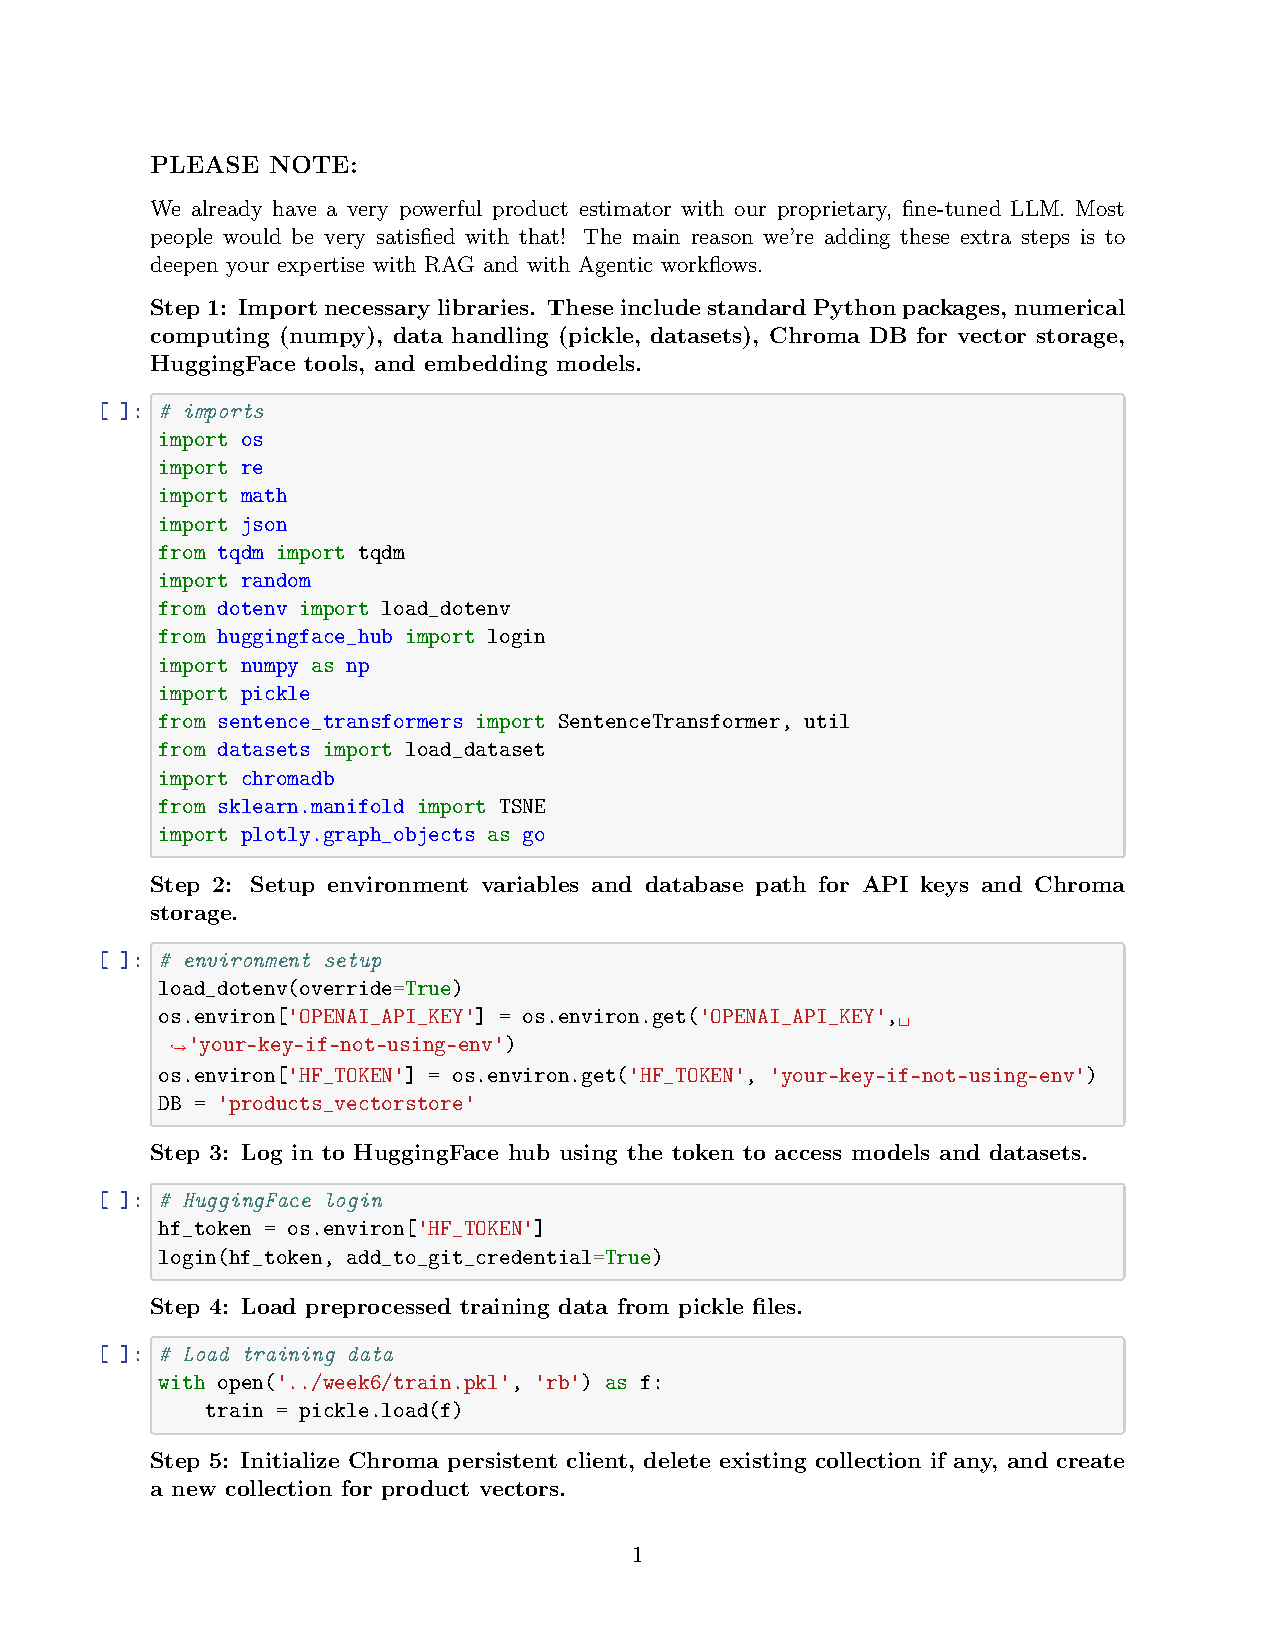
\includepdf[pages=-]{DAY2.pdf}



\section{Hallmarks of an Agentic AI Solution}
\begin{tcolorbox}[title={1. Decomposition of Larger Problems into Smaller Steps}, colback=blue!5!white, colframe=blue!75!black]
An \textbf{Agentic AI system} decomposes complex problems into smaller, manageable steps. Each step is handled by an \textit{independent agent} or \textit{specialized process}, allowing for:  
\begin{itemize}
    \item \textbf{Parallel processing} for faster execution.
    \item \textbf{Error reduction} by isolating tasks.
    \item \textbf{Task modularity} to reuse and recombine solutions.
    \item \textit{Scalable problem solving} for multi-domain challenges.
\end{itemize}
This approach ensures that large goals can be achieved efficiently without overwhelming any single component.
\end{tcolorbox}
\vspace{0.5cm}
\begin{tcolorbox}[title={2. Use of Tools, Function Calling, and Structured Outputs}, colback=green!5!white, colframe=green!75!black]
Agents can call \textit{external tools}, \textit{APIs}, or defined functions to extend their capabilities. Structured outputs ensure clear and reliable results. Key benefits include:  
\begin{itemize}
    \item \textbf{Precision:} Outputs like JSON or tables can be directly processed.
    \item \textbf{Reliability:} Reduces ambiguity in multi-agent workflows.
    \item \textbf{Interoperability:} Allows agents to communicate results seamlessly.
    \item \textit{Error handling:} Structured formats make it easier to validate and parse responses.
\end{itemize}
\end{tcolorbox}
\vspace{0.5cm}

\begin{tcolorbox}[title={3. Collaborative Agent Environment}, colback=orange!5!white, colframe=orange!75!black]
Agents operate in a shared environment enabling \textbf{collaboration and coordination}:  
\begin{itemize}
    \item \textbf{Specialized knowledge:} Different agents contribute unique skills.
    \item \textbf{Task distribution:} Efficient division of labor for complex goals.
    \item \textit{Real-time communication:} Agents exchange updates to optimize outcomes.
    \item \textit{Conflict resolution:} Conflicting suggestions can be reconciled by higher-level agents.
\end{itemize}
Collaboration enhances overall system performance beyond the capability of any single agent.
\end{tcolorbox}
\vspace{0.5cm}

\begin{tcolorbox}[title={4. Planning and Coordination Agent}, colback=red!5!white, colframe=red!75!black]
A \textbf{planning agent} orchestrates activities across all agents:  
\begin{itemize}
    \item Determines the sequence of tasks based on dependencies.
    \item Dynamically adjusts plans according to intermediate results.
    \item Prioritizes critical steps to achieve goals efficiently.
    \item Monitors progress and reallocates resources as needed.
\end{itemize}
This ensures that complex workflows are executed coherently and reliably.
\end{tcolorbox}
\vspace{0.5cm}

\begin{tcolorbox}[title={5. Autonomy and Persistent Memory}, colback=purple!5!white, colframe=purple!75!black]
Agentic AI demonstrates \textbf{autonomy} and maintains \textit{persistent memory}, which allows:  
\begin{itemize}
    \item \textbf{Independent operation} without constant human intervention.
    \item \textbf{Learning from past interactions} to improve decision-making.
    \item Retention of critical information across sessions for long-term planning.
    \item \textit{Cumulative knowledge growth}, enabling adaptation to new situations.
    \item Capability to handle multi-step and long-horizon tasks effectively.
\end{itemize}
\end{tcolorbox}
\vspace{1cm}
\includegraphics[width=1\textwidth]{hallmark.png}

% Part 1: System Overview and Architecture
\chapter{System Overview and Architecture}

\section{Introduction}

This document provides an exhaustive technical analysis of a sophisticated Python-based multi-agent system designed for automated deal discovery, analysis, and notification. The system represents a compelling example of modern software engineering principles, combining object-oriented programming, machine learning, web scraping, API integration, and distributed computing into a cohesive, production-ready application.

The system operates as an intelligent deal-hunting assistant that continuously monitors RSS feeds from deal websites, applies multiple machine learning models to estimate product prices, identifies potentially valuable deals by comparing estimated prices with actual prices, and automatically notifies users of significant opportunities through various messaging channels.

\subsection{System Purpose and Goals}

The primary objective of this multi-agent system is to automate the process of finding profitable deals across multiple online retailers. The system accomplishes this through several key capabilities:

\begin{enumerate}[itemsep=0.5em]
\item \textbf{Autonomous Deal Discovery}: Continuously monitors RSS feeds from deal aggregation websites like DealNews to identify new product offers
\item \textbf{Intelligent Price Estimation}: Employs multiple machine learning approaches including ensemble methods, fine-tuned language models, and traditional ML algorithms to predict fair market prices
\item \textbf{Opportunity Analysis}: Calculates potential savings by comparing estimated fair prices against offered deal prices
\item \textbf{Automated Notification}: Delivers alerts through multiple channels (SMS, push notifications) when significant deals are identified
\item \textbf{Memory Management}: Maintains awareness of previously processed deals to avoid duplicate notifications
\end{enumerate}

\subsection{Technical Architecture Overview}

The system employs a modular, agent-based architecture where each component (agent) has specialized responsibilities. This design pattern promotes separation of concerns, maintainability, and scalability. The architecture can be categorized into several layers:

\begin{itemize}[itemsep=0.5em]
\item \textbf{Orchestration Layer}: The PlanningAgent coordinates the entire workflow
\item \textbf{Data Acquisition Layer}: ScannerAgent and deals processing handle external data retrieval
\item \textbf{Machine Learning Layer}: Multiple specialized agents provide price estimation using different ML approaches
\item \textbf{Communication Layer}: MessagingAgent handles user notifications
\item \textbf{Foundation Layer}: Base Agent class and data models provide common functionality
\end{itemize}

\section{Agent-Based Architecture}

\subsection{The Agent Pattern}

The system implements the Agent design pattern, where each agent is an autonomous unit capable of:
\begin{itemize}
\item Independent operation with well-defined responsibilities
\item Communication and coordination with other agents
\item State management and decision making
\item Logging and monitoring of its activities
\end{itemize}

All agents inherit from a common \texttt{Agent} base class that provides:
\begin{itemize}
\item Colored console logging for visual differentiation during runtime
\item Consistent naming conventions
\item Standardized communication protocols
\end{itemize}

\subsection{System Components}

\begin{figure}[htbp]
\centering
\begin{tikzpicture}[scale=0.6, transform shape,
    node distance=2cm,
    box/.style={rectangle, draw=black!50, fill=blue!10, thick, minimum width=2.5cm, minimum height=1cm, text centered},
    arrow/.style={->, >=stealth, thick}
]

% Define nodes
\node[box, fill=green!20] (planning) {Planning Agent};
\node[box, below left=of planning, fill=cyan!20] (scanner) {Scanner Agent};
\node[box, below=of planning, fill=yellow!20] (ensemble) {Ensemble Agent};
\node[box, below right=of planning, fill=white] (messaging) {Messaging Agent};

% Ensemble sub-agents
\node[box, below left=of ensemble, fill=red!20] (specialist) {Specialist Agent};
\node[box, below=of ensemble, fill=blue!20] (frontier) {Frontier Agent};
\node[box, below right=of ensemble, fill=magenta!20] (randomforest) {Random Forest Agent};

% Data components
\node[box, left=of scanner, fill=orange!20] (deals) {Deal Processing};
\node[box, right=of messaging, fill=gray!20] (notifications) {External APIs};

% Draw arrows
\draw[arrow] (planning) -- (scanner);
\draw[arrow] (planning) -- (ensemble);
\draw[arrow] (planning) -- (messaging);

\draw[arrow] (ensemble) -- (specialist);
\draw[arrow] (ensemble) -- (frontier);
\draw[arrow] (ensemble) -- (randomforest);

\draw[arrow] (scanner) -- (deals);
\draw[arrow] (messaging) -- (notifications);

% Add labels for data flow
\node[above, font=\footnotesize] at ($(planning)!0.5!(scanner)$) {Deal Requests};
\node[above, font=\footnotesize] at ($(planning)!0.5!(ensemble)$) {Price Estimation};
\node[above, font=\footnotesize] at ($(planning)!0.5!(messaging)$) {Notifications};

\end{tikzpicture}
\caption{High-Level System Architecture showing agent relationships and data flow}
\label{fig:system_architecture}
\end{figure}


\subsubsection{Core Agents}

\paragraph{PlanningAgent (Orchestrator)}
The PlanningAgent serves as the system's central coordinator, implementing the main workflow logic. It instantiates and manages all other agents, coordinates their interactions, and makes high-level decisions about deal processing. The PlanningAgent embodies the Command pattern, orchestrating a complex sequence of operations across multiple specialized components.

\paragraph{ScannerAgent (Data Acquisition)}
Responsible for monitoring external RSS feeds and identifying new deals. The system includes two implementations:
\begin{itemize}
\item \texttt{ScannerAgent}: Uses OpenAI's structured output API
\item \texttt{ScannerAgentLangChain}: Uses Google's Gemini via LangChain framework
\end{itemize}
Both implementations extract deal information and convert unstructured web data into structured \texttt{Deal} objects.

\paragraph{EnsembleAgent (ML Coordinator)}
Implements an ensemble machine learning approach by coordinating three different price estimation models. It uses a meta-learning approach where a Linear Regression model combines predictions from specialist models to produce final price estimates.

\paragraph{MessagingAgent (Communication)}
Handles external communications through multiple channels including SMS (via Twilio) and push notifications (via Pushover). This agent implements the Publisher pattern, broadcasting deal alerts to configured endpoints.

\subsubsection{Specialized ML Agents}

\paragraph{SpecialistAgent (Fine-tuned Model)}
Utilizes a remotely-hosted, fine-tuned language model via Modal's cloud platform. This agent represents the most sophisticated ML approach in the system, leveraging domain-specific training for price estimation.

\paragraph{FrontierAgent (RAG-based LLM)}
Implements a Retrieval-Augmented Generation (RAG) approach using vector similarity search. It finds similar products in a ChromaDB vector store and uses this context to inform price predictions via OpenAI's GPT models.

\paragraph{RandomForestAgent (Traditional ML)}
Uses a pre-trained Random Forest model combined with sentence embeddings for price prediction. This represents a more traditional machine learning approach compared to the LLM-based agents.

\section{Data Flow and System Interactions}

\subsection{Primary Workflow}

The system operates through a well-defined workflow that demonstrates sophisticated inter-agent communication:

\begin{enumerate}
\item \textbf{Initialization Phase}: PlanningAgent instantiates all required agents, each performing their specific setup routines
\item \textbf{Deal Discovery}: ScannerAgent monitors RSS feeds and extracts new deals not in memory
\item \textbf{Price Analysis}: For each deal, EnsembleAgent coordinates price estimation across all ML agents
\item \textbf{Opportunity Calculation}: System compares estimated prices with deal prices to calculate potential savings
\item \textbf{Decision Making}: PlanningAgent determines whether deals meet threshold criteria for notification
\item \textbf{User Notification}: MessagingAgent delivers alerts through configured channels
\end{enumerate}

\subsection{Data Models}

The system employs Pydantic models for robust data validation and serialization:

\begin{lstlisting}[caption=Core Data Models]
class Deal(BaseModel):
    """Structured representation of a deal"""
    product_description: str
    price: float
    url: str

class DealSelection(BaseModel):
    """Container for multiple deals"""
    deals: List[Deal]

class Opportunity(BaseModel):
    """Represents a potential profitable deal"""
    deal: Deal
    estimate: float  # ML-predicted price
    discount: float  # Estimated savings
\end{lstlisting}

\section{Advanced System Features}

\subsection{Machine Learning Integration}

The system showcases multiple machine learning paradigms:

\begin{itemize}
\item \textbf{Ensemble Methods}: Meta-learning approach combining multiple models
\item \textbf{Fine-tuned LLMs}: Domain-specific language model training
\item \textbf{RAG (Retrieval-Augmented Generation)}: Vector similarity search with LLM reasoning
\item \textbf{Traditional ML}: Scikit-learn Random Forest with feature engineering
\item \textbf{Vector Embeddings}: Sentence transformers for semantic similarity
\end{itemize}

\subsection{External Service Integration}

The system integrates with multiple external services:

\begin{table}[htbp]
\centering
\begin{tabular}{@{}lll@{}}
\toprule
Service Category & Implementation & Purpose \\
\midrule
LLM APIs & OpenAI, DeepSeek, Google Gemini & Price estimation and reasoning \\
Vector Database & ChromaDB & Similarity search for RAG \\
Cloud Computing & Modal & Remote model hosting \\
Messaging & Twilio, Pushover & User notifications \\
Data Sources & RSS Feeds & Deal discovery \\
\bottomrule
\end{tabular}
\caption{External Service Integrations}
\label{tab:external_services}
\end{table}

\subsection{Error Handling and Robustness}

The system implements several robustness mechanisms:

\begin{itemize}
\item \textbf{Graceful Degradation}: Continues operation if individual agents fail
\item \textbf{Data Validation}: Pydantic models ensure data integrity
\item \textbf{Rate Limiting}: Built-in delays prevent API abuse
\item \textbf{Memory Management}: Tracks processed deals to avoid duplicates
\item \textbf{Logging}: Comprehensive logging for debugging and monitoring
\end{itemize}

\section{Architectural Patterns}

\subsection{Design Patterns Implemented}

The system demonstrates several well-known design patterns:

\begin{description}
\item[Agent Pattern] Each component operates autonomously with defined responsibilities
\item[Strategy Pattern] Multiple ML algorithms can be swapped in the ensemble
\item[Command Pattern] PlanningAgent orchestrates complex operations
\item[Factory Pattern] Agent instantiation and configuration
\item[Observer Pattern] Event-driven notifications and logging
\item[Template Method] Base Agent class defines common behavior
\end{description}

\subsection{SOLID Principles}

The architecture adheres to SOLID principles:

\begin{itemize}
\item \textbf{Single Responsibility}: Each agent has one primary function
\item \textbf{Open/Closed}: New agents can be added without modifying existing code
\item \textbf{Liskov Substitution}: All agents can be used polymorphically
\item \textbf{Interface Segregation}: Agents depend only on methods they use
\item \textbf{Dependency Inversion}: High-level modules don't depend on low-level details
\end{itemize}

\section{System Scalability and Performance}

\subsection{Scalability Considerations}

The modular architecture enables several scaling strategies:

\begin{itemize}
\item \textbf{Horizontal Scaling}: Agents can be distributed across multiple processes/machines
\item \textbf{Load Balancing}: Multiple instances of compute-intensive agents
\item \textbf{Caching}: Vector embeddings and model predictions can be cached
\item \textbf{Asynchronous Processing}: Background tasks for non-critical operations
\end{itemize}

\subsection{Performance Characteristics}

Key performance aspects include:

\begin{itemize}
\item \textbf{I/O Bound Operations}: RSS feed parsing, API calls
\item \textbf{CPU Bound Operations}: ML model inference, text processing
\item \textbf{Memory Usage}: Vector embeddings, model weights
\item \textbf{Network Latency}: External API dependencies
\end{itemize}

\section{Security and Privacy}

\subsection{Security Measures}

The system implements several security best practices:

\begin{itemize}
\item \textbf{API Key Management}: Environment variables for sensitive credentials
\item \textbf{Input Validation}: Pydantic models prevent injection attacks
\item \textbf{Rate Limiting}: Prevents abuse of external services
\item \textbf{Error Sanitization}: Logs don't expose sensitive information
\end{itemize}

\subsection{Privacy Considerations}

\begin{itemize}
\item \textbf{Data Minimization}: Only necessary data is collected and stored
\item \textbf{External Dependencies}: User data may be sent to third-party APIs
\item \textbf{Logging Practices}: Personal information excluded from logs
\end{itemize}

\section{Chapter Summary}

This chapter provided a comprehensive overview of the Python multi-agent deal discovery system. We explored:

\begin{itemize}
\item The system's purpose as an automated deal-hunting assistant
\item The agent-based architecture promoting modularity and maintainability  
\item The sophisticated integration of multiple machine learning approaches
\item The robust data models and external service integrations
\item The adherence to established design patterns and software engineering principles
\end{itemize}

The system represents a excellent example of modern Python development, combining object-oriented design, machine learning, web technologies, and distributed computing into a cohesive, production-ready application. The modular architecture ensures that the system can evolve and scale while maintaining reliability and performance.

In the subsequent chapters, we will dive deeper into each component, examining the implementation details, Python language features utilized, class hierarchies, and the intricate interactions between agents that make this system function as a unified whole.

% Part 2: Detailed File-by-File Analysis  
\chapter{File-by-File Detailed Analysis}

This chapter provides an exhaustive examination of each Python file in the multi-agent deal discovery system. We will analyze every class, function, method, and their interconnections, demonstrating how the modular architecture enables sophisticated functionality through careful component design.

\section{agent.py - The Foundation Base Class}

The \texttt{agent.py} file establishes the foundational infrastructure for the entire agent system. This file demonstrates fundamental object-oriented programming principles and serves as the template for all specialized agents.

\subsection{File Structure and Imports}

\begin{lstlisting}[caption=agent.py - Complete File Analysis]
import logging

class Agent:
    """
    An abstract superclass for Agents
    Used to log messages in a way that can identify each Agent
    """

    # Foreground colors
    RED = '\033[31m'
    GREEN = '\033[32m'
    YELLOW = '\033[33m'
    BLUE = '\033[34m'
    MAGENTA = '\033[35m'
    CYAN = '\033[36m'
    WHITE = '\033[37m'
    
    # Background color
    BG_BLACK = '\033[40m'
    
    # Reset code to return to default color
    RESET = '\033[0m'

    name: str = ""
    color: str = '\033[37m'

    def log(self, message):
        """
        Log this as an info message, identifying the agent
        """
        color_code = self.BG_BLACK + self.color
        message = f"[{self.name}] {message}"
        logging.info(color_code + message + self.RESET)
\end{lstlisting}

\subsection{Class Analysis: Agent}

\subsubsection{Class-Level Attributes}

The Agent class defines several class-level constants using ANSI escape sequences for terminal color formatting:

\begin{itemize}
\item \textbf{Color Constants}: Seven foreground colors (RED through WHITE) defined as class constants
\item \textbf{Background Color}: BG\_BLACK provides consistent background formatting
\item \textbf{Reset Code}: RESET returns terminal to default formatting
\item \textbf{Instance Attributes}: 
  \begin{itemize}
  \item \texttt{name: str} - Identifier for the specific agent instance
  \item \texttt{color: str} - Default color scheme for the agent's log output
  \end{itemize}
\end{itemize}

\paragraph{Python Concepts Demonstrated}
\begin{itemize}
\item \textbf{Class Constants}: Using uppercase naming convention for immutable values
\item \textbf{Type Annotations}: Modern Python typing for \texttt{name} and \texttt{color}
\item \textbf{Default Values}: Providing sensible defaults for instance attributes
\item \textbf{ANSI Escape Sequences}: Terminal control codes for colored output
\end{itemize}

\subsubsection{Method Analysis: log()}

The \texttt{log()} method provides centralized logging functionality:

\begin{lstlisting}[caption=Detailed log() Method Analysis]
def log(self, message):
    """
    Log this as an info message, identifying the agent
    """
    color_code = self.BG_BLACK + self.color
    message = f"[{self.name}] {message}"
    logging.info(color_code + message + self.RESET)
\end{lstlisting}

\paragraph{Step-by-Step Execution Analysis}
\begin{enumerate}
\item \textbf{Color Code Construction}: Concatenates background and foreground color codes
\item \textbf{Message Formatting}: Uses f-string interpolation to prepend agent name
\item \textbf{Logging Call}: Utilizes Python's logging module with INFO level
\item \textbf{Color Reset}: Ensures terminal formatting returns to normal after message
\end{enumerate}

\paragraph{Memory and Object Interaction}
\begin{itemize}
\item \textbf{String Concatenation}: Creates new string objects for color\_code and formatted message
\item \textbf{Method Resolution}: \texttt{self.name} and \texttt{self.color} trigger attribute lookup
\item \textbf{Module Function Call}: \texttt{logging.info()} invokes standard library function
\item \textbf{Garbage Collection}: Temporary strings become eligible for cleanup after method completion
\end{itemize}

\subsection{Inter-File Relationships}

The Agent class serves as the superclass for all specialized agents:
\begin{itemize}
\item \textbf{EnsembleAgent} inherits from Agent
\item \textbf{FrontierAgent} inherits from Agent  
\item \textbf{RandomForestAgent} inherits from Agent
\item \textbf{SpecialistAgent} inherits from Agent
\item \textbf{MessagingAgent} inherits from Agent
\item \textbf{PlanningAgent} inherits from Agent
\item \textbf{ScannerAgent} inherits from Agent
\end{itemize}

\section{deals.py - Data Models and External Integration}

The \texttt{deals.py} file implements the core data structures and external API integration logic. This file demonstrates advanced Python features including Pydantic models, web scraping, RSS parsing, and object-oriented design patterns.

\subsection{Imports and Dependencies}

\begin{lstlisting}[caption=deals.py - Import Analysis]
from pydantic import BaseModel
from typing import List, Dict, Self
from bs4 import BeautifulSoup
import re
import feedparser
from tqdm import tqdm
import requests
import time
\end{lstlisting}

\paragraph{Import Analysis}
\begin{itemize}
\item \textbf{pydantic.BaseModel}: Provides data validation and serialization
\item \textbf{typing}: Modern type hints for generic collections and self-references
\item \textbf{BeautifulSoup}: HTML/XML parsing for web scraping
\item \textbf{re}: Regular expression processing for text extraction
\item \textbf{feedparser}: RSS/Atom feed parsing
\item \textbf{tqdm}: Progress bar for user-friendly feedback
\item \textbf{requests}: HTTP client for web requests
\item \textbf{time}: Sleep functionality for rate limiting
\end{itemize}

\subsection{Global Configuration}

\begin{lstlisting}[caption=RSS Feed Configuration]
feeds = [
    "https://www.dealnews.com/c142/Electronics/?rss=1",
    "https://www.dealnews.com/c39/Computers/?rss=1", 
    "https://www.dealnews.com/c238/Automotive/?rss=1",
    "https://www.dealnews.com/f1912/Smart-Home/?rss=1",
    "https://www.dealnews.com/c196/Home-Garden/?rss=1",
]
\end{lstlisting}

This module-level list defines the RSS feeds to monitor, demonstrating configuration through global constants.

\subsection{Utility Function: extract()}

\begin{lstlisting}[caption=HTML Text Extraction Function]
def extract(html_snippet: str) -> str:
    """
    Use Beautiful Soup to clean up this HTML snippet and extract useful text
    """
    soup = BeautifulSoup(html_snippet, 'html.parser')
    snippet_div = soup.find('div', class_='snippet summary')
    
    if snippet_div:
        description = snippet_div.get_text(strip=True)
        description = BeautifulSoup(description, 'html.parser').get_text()
        description = re.sub('<[^<]+?>', '', description)
        result = description.strip()
    else:
        result = html_snippet
    return result.replace('\n', ' ')
\end{lstlisting}

\paragraph{Function Analysis}
\begin{enumerate}
\item \textbf{HTML Parsing}: Creates BeautifulSoup object from HTML string
\item \textbf{Element Search}: Finds specific div with 'snippet summary' class
\item \textbf{Text Extraction}: Converts HTML elements to plain text
\item \textbf{HTML Tag Removal}: Uses regex to remove remaining HTML tags
\item \textbf{Whitespace Cleanup}: Normalizes spacing and removes newlines
\end{enumerate}

\paragraph{Error Handling Strategy}
The function implements graceful degradation - if the expected HTML structure isn't found, it returns the original input rather than failing.

\subsection{Class Analysis: ScrapedDeal}

\begin{lstlisting}[caption=ScrapedDeal Class Implementation]
class ScrapedDeal:
    """
    A class to represent a Deal retrieved from an RSS feed
    """
    category: str
    title: str
    summary: str
    url: str
    details: str
    features: str

    def __init__(self, entry: Dict[str, str]):
        """
        Populate this instance based on the provided dict
        """
        self.title = entry['title']
        self.summary = extract(entry['summary'])
        self.url = entry['links'][0]['href']
        stuff = requests.get(self.url).content
        soup = BeautifulSoup(stuff, 'html.parser')
        content = soup.find('div', class_='content-section').get_text()
        content = content.replace('\nmore', '').replace('\n', ' ')
        if "Features" in content:
            self.details, self.features = content.split("Features")
        else:
            self.details = content
            self.features = ""
\end{lstlisting}

\paragraph{Constructor Analysis}
The \texttt{\_\_init\_\_} method demonstrates complex initialization logic:

\begin{enumerate}
\item \textbf{Basic Attribute Assignment}: Direct mapping from RSS entry
\item \textbf{HTML Processing}: Uses extract() function for summary cleanup
\item \textbf{URL Extraction}: Navigates nested dictionary structure for URL
\item \textbf{HTTP Request}: Fetches full webpage content
\item \textbf{Content Parsing}: Extracts specific div content
\item \textbf{Text Processing}: Cleans and normalizes extracted text
\item \textbf{Content Separation}: Splits content into details and features sections
\end{enumerate}

\paragraph{Python Concepts Demonstrated}
\begin{itemize}
\item \textbf{Type Hints}: All attributes have explicit type annotations
\item \textbf{Dictionary Access}: Multiple patterns for accessing nested data
\item \textbf{String Methods}: replace(), split(), strip() for text processing
\item \textbf{HTTP Requests}: Web scraping using requests library
\item \textbf{Conditional Logic}: Feature separation with fallback handling
\end{itemize}

\subsubsection{Instance Methods}

\begin{lstlisting}[caption=ScrapedDeal Instance Methods]
def __repr__(self):
    """
    Return a string to describe this deal
    """
    return f"<{self.title}>"

def describe(self):
    """
    Return a longer string to describe this deal for use in calling a model
    """
    return f"Title: {self.title}\nDetails: {self.details.strip()}\nFeatures: {self.features.strip()}\nURL: {self.url}"
\end{lstlisting}

\paragraph{Method Analysis}
\begin{itemize}
\item \textbf{\_\_repr\_\_()}: Provides developer-friendly string representation
\item \textbf{describe()}: Generates formatted text for ML model consumption
\end{itemize}

\subsubsection{Class Method: fetch()}

\begin{lstlisting}[caption=ScrapedDeal.fetch() Class Method]
@classmethod
def fetch(cls, show_progress : bool = False) -> List[Self]:
    """
    Retrieve all deals from the selected RSS feeds
    """
    deals = []
    feed_iter = tqdm(feeds) if show_progress else feeds
    for feed_url in feed_iter:
        feed = feedparser.parse(feed_url)
        for entry in feed.entries[:10]:
            deals.append(cls(entry))
            time.sleep(0.5)
    return deals
\end{lstlisting}

\paragraph{Class Method Analysis}
\begin{enumerate}
\item \textbf{Class Method Decorator}: Uses \texttt{@classmethod} to create alternative constructor
\item \textbf{Progress Bar Integration}: Conditional \texttt{tqdm} usage based on parameter
\item \textbf{RSS Feed Processing}: Iterates through configured feeds
\item \textbf{Entry Limitation}: Processes only first 10 entries per feed
\item \textbf{Rate Limiting}: 0.5-second delay between requests
\item \textbf{Instance Creation}: Uses \texttt{cls()} to create instances of current class
\end{enumerate}

\vspace{1em}

\paragraph{Return Type Analysis}
\begin{itemize}
\item \textbf{List[Self]}: Uses modern Python typing for self-referential return type
\item \textbf{Generic Type}: Maintains type safety across inheritance hierarchies
\end{itemize}

\subsection{Pydantic Models}

\begin{lstlisting}[caption=Pydantic Model Definitions]
class Deal(BaseModel):
    """
    A class to Represent a Deal with a summary description
    """
    product_description: str
    price: float
    url: str

class DealSelection(BaseModel):
    """
    A class to Represent a list of Deals
    """
    deals: List[Deal]

class Opportunity(BaseModel):
    """
    A class to represent a possible opportunity: a Deal where we estimate
    it should cost more than it's being offered
    """
    deal: Deal
    estimate: float
    discount: float
\end{lstlisting}

\paragraph{Pydantic Model Benefits}
\begin{itemize}
\item \textbf{Automatic Validation}: Type checking and constraint enforcement
\item \textbf{JSON Serialization}: Built-in conversion to/from JSON
\item \textbf{IDE Support}: Enhanced autocomplete and type checking
\item \textbf{Documentation}: Automatic schema generation
\item \textbf{Performance}: Optimized validation using Rust backend
\end{itemize}

\section{ensemble\_agent.py - Meta-Learning Orchestration}

The EnsembleAgent represents a sophisticated machine learning approach, implementing meta-learning by combining predictions from multiple specialized models.

\subsection{File Structure and Dependencies}
\vspace{1em}

\begin{lstlisting}[caption=ensemble\_agent.py - Complete Implementation]
import pandas as pd
from sklearn.linear_model import LinearRegression
import joblib

from agents.agent import Agent
from agents.specialist_agent import SpecialistAgent
from agents.frontier_agent import FrontierAgent
from agents.random_forest_agent import RandomForestAgent

class EnsembleAgent(Agent):

    name = "Ensemble Agent"
    color = Agent.YELLOW
    
    def __init__(self, collection):
        """
        Create an instance of Ensemble, by creating each of the models
        And loading the weights of the Ensemble
        """
        self.log("Initializing Ensemble Agent")
        self.specialist = SpecialistAgent()
        self.frontier = FrontierAgent(collection)
        self.random_forest = RandomForestAgent()
        self.model = joblib.load('ensemble_model.pkl')
        self.log("Ensemble Agent is ready")

    def price(self, description: str) -> float:
        """
        Run this ensemble model
        Ask each of the models to price the product
        Then use the Linear Regression model to return the weighted price
        :param description: the description of a product
        :return: an estimate of its price
        """
        self.log("Running Ensemble Agent - collaborating with specialist, frontier and random forest agents")
        specialist = self.specialist.price(description)
        frontier = self.frontier.price(description)
        random_forest = self.random_forest.price(description)
        X = pd.DataFrame({
            'Specialist': [specialist],
            'Frontier': [frontier],
            'RandomForest': [random_forest],
            'Min': [min(specialist, frontier, random_forest)],
            'Max': [max(specialist, frontier, random_forest)],
        })
        y = max(0, self.model.predict(X)[0])
        self.log(f"Ensemble Agent complete - returning \$${y:.2f}")
        return y
\end{lstlisting}
\vspace{1em}

\subsection{Class Analysis: EnsembleAgent}

\paragraph{Inheritance Relationship}
\begin{itemize}
\item \textbf{Parent Class}: Inherits from Agent base class
\item \textbf{Class Attributes}: Overrides name and color from parent
\item \textbf{Method Override}: Inherits log() method without modification
\end{itemize}

\paragraph{Constructor Analysis}
The constructor demonstrates dependency injection and composition patterns:

\begin{enumerate}
\item \textbf{Logging Initialization}: Calls inherited log() method
\item \textbf{Agent Composition}: Creates instances of three specialized agents
\item \textbf{Model Loading}: Loads pre-trained ensemble model using joblib
\item \textbf{Completion Logging}: Confirms successful initialization
\end{enumerate}

\paragraph{Composition vs. Inheritance}
The EnsembleAgent uses composition rather than multiple inheritance to combine different ML approaches, demonstrating sound object-oriented design.

\subsubsection{Method Analysis: price()}

\begin{lstlisting}[caption=Ensemble Price Prediction Method]
def price(self, description: str) -> float:
    self.log("Running Ensemble Agent - collaborating with specialist, frontier and random forest agents")
    specialist = self.specialist.price(description)
    frontier = self.frontier.price(description)
    random_forest = self.random_forest.price(description)
    X = pd.DataFrame({
        'Specialist': [specialist],
        'Frontier': [frontier], 
        'RandomForest': [random_forest],
        'Min': [min(specialist, frontier, random_forest)],
        'Max': [max(specialist, frontier, random_forest)],
    })
    y = max(0, self.model.predict(X)[0])
    self.log(f"Ensemble Agent complete - returning ${y:.2f}")
    return y
\end{lstlisting}

\paragraph{Step-by-Step Execution Analysis}
\begin{enumerate}
\item \textbf{Logging Start}: Announces collaboration with other agents
\item \textbf{Specialist Prediction}: Calls SpecialistAgent.price() method
\item \textbf{Frontier Prediction}: Calls FrontierAgent.price() method  
\item \textbf{Random Forest Prediction}: Calls RandomForestAgent.price() method
\item \textbf{Feature Engineering}: Creates DataFrame with original predictions plus min/max
\item \textbf{Ensemble Prediction}: Uses meta-model to combine predictions
\item \textbf{Non-negative Constraint}: Ensures price cannot be negative
\item \textbf{Result Logging}: Reports final prediction with formatting
\end{enumerate}

\paragraph{Machine Learning Concepts}
\begin{itemize}
\item \textbf{Ensemble Methods}: Combining multiple models for better performance
\item \textbf{Meta-Learning}: Using a model to learn how to combine other models
\item \textbf{Feature Engineering}: Creating additional features (min, max) from base predictions
\item \textbf{Stacking}: Specific ensemble technique using a meta-learner
\end{itemize}

\paragraph{Data Flow Analysis}
\begin{itemize}
\item \textbf{Input}: Single string description
\item \textbf{Processing}: Three parallel predictions + statistical features
\item \textbf{Combination}: Linear regression meta-model
\item \textbf{Output}: Single float price prediction
\end{itemize}

\section{frontier\_agent.py - RAG-Based LLM Integration}

The FrontierAgent implements Retrieval-Augmented Generation (RAG), combining vector search with large language model reasoning for price estimation.

\subsection{Import Dependencies}

\begin{lstlisting}[caption=frontier\_agent.py - Dependencies]
import os
import re
import math
import json
from typing import List, Dict
from openai import OpenAI
from sentence_transformers import SentenceTransformer
from datasets import load_dataset
import chromadb
from items import Item
from testing import Tester
from agents.agent import Agent
\end{lstlisting}

\paragraph{Import Analysis}
\begin{itemize}
\item \textbf{Standard Library}: os, re, math, json for basic functionality
\item \textbf{Type Hints}: typing module for type annotations
\item \textbf{OpenAI Integration}: Direct API client for LLM calls
\item \textbf{Vector Embeddings}: SentenceTransformer for semantic similarity
\item \textbf{Vector Database}: ChromaDB for similarity search
\item \textbf{Base Class}: Agent inheritance
\end{itemize}

\subsection{Class Analysis: FrontierAgent}

\begin{lstlisting}[caption=FrontierAgent Class Structure]
class FrontierAgent(Agent):

    name = "Frontier Agent"
    color = Agent.BLUE

    MODEL = "gpt-4o-mini"
    
    def __init__(self, collection):
        """
        Set up this instance by connecting to OpenAI or DeepSeek, to the Chroma Datastore,
        And setting up the vector encoding model
        """
        self.log("Initializing Frontier Agent")
        deepseek_api_key = os.getenv("DEEPSEEK_API_KEY")
        if deepseek_api_key:
            self.client = OpenAI(api_key=deepseek_api_key, base_url="https://api.deepseek.com")
            self.MODEL = "deepseek-chat"
            self.log("Frontier Agent is set up with DeepSeek")
        else:
            self.client = OpenAI()
            self.MODEL = "gpt-4o-mini"
            self.log("Frontier Agent is setting up with OpenAI")
        self.collection = collection
        self.model = SentenceTransformer('sentence-transformers/all-MiniLM-L6-v2')
        self.log("Frontier Agent is ready")
\end{lstlisting}

\paragraph{Constructor Analysis}
\begin{enumerate}
\item \textbf{Environment Variable Check}: Determines LLM provider based on API key availability
\item \textbf{Conditional Client Creation}: Creates appropriate OpenAI client instance
\item \textbf{Model Selection}: Sets MODEL constant based on provider
\item \textbf{ChromaDB Integration}: Stores collection reference for vector search
\item \textbf{Embedding Model}: Initializes SentenceTransformer for vector encoding
\end{enumerate}

\paragraph{Design Patterns}
\begin{itemize}
\item \textbf{Strategy Pattern}: Interchangeable LLM providers (OpenAI vs DeepSeek)
\item \textbf{Dependency Injection}: ChromaDB collection passed in constructor
\item \textbf{Factory Pattern}: Conditional object creation based on environment
\end{itemize}

\subsubsection{Method Analysis: make\_context()}

\begin{lstlisting}[caption=Context Generation Method]
def make_context(self, similars: List[str], prices: List[float]) -> str:
    """
    Create context that can be inserted into the prompt
    :param similars: similar products to the one being estimated
    :param prices: prices of the similar products
    :return: text to insert in the prompt that provides context
    """
    message = "To provide some context, here are some other items that might be similar to the item you need to estimate.\n\n"
    for similar, price in zip(similars, prices):
        message += f"Potentially related product:\n{similar}\nPrice is ${price:.2f}\n\n"
    return message
\end{lstlisting}

\paragraph{Method Analysis}
\begin{itemize}
\item \textbf{Template Building}: Constructs structured prompt template
\item \textbf{List Iteration}: Uses zip() to pair similar products with prices
\item \textbf{String Formatting}: f-string interpolation for price formatting
\item \textbf{Context Injection}: Prepares RAG context for LLM consumption
\end{itemize}

\subsubsection{Method Analysis: messages\_for()}

\begin{lstlisting}[caption=OpenAI Message Construction]
def messages_for(self, description: str, similars: List[str], prices: List[float]) -> List[Dict[str, str]]:
    """
    Create the message list to be included in a call to OpenAI
    With the system and user prompt
    """
    system_message = "You estimate prices of items. Reply only with the price, no explanation"
    user_prompt = self.make_context(similars, prices)
    user_prompt += "And now the question for you:\n\n"
    user_prompt += "How much does this cost?\n\n" + description
    return [
        {"role": "system", "content": system_message},
        {"role": "user", "content": user_prompt},
        {"role": "assistant", "content": "Price is $"}
    ]
\end{lstlisting}

\paragraph{Prompt Engineering Analysis}
\begin{itemize}
\item \textbf{System Prompt}: Clear, concise instructions for the LLM
\item \textbf{Context Integration}: Incorporates RAG results into user prompt
\item \textbf{Few-Shot Learning}: Provides examples through similar products
\item \textbf{Response Priming}: Pre-fills assistant response to guide output format
\end{itemize}

\subsubsection{Method Analysis: find\_similars()}

\begin{lstlisting}[caption=Vector Similarity Search]
def find_similars(self, description: str):
    """
    Return a list of items similar to the given one by looking in the Chroma datastore
    """
    self.log("Frontier Agent is performing a RAG search of the Chroma datastore to find 5 similar products")
    vector = self.model.encode([description])
    results = self.collection.query(query_embeddings=vector.astype(float).tolist(), n_results=5)
    documents = results['documents'][0][:]
    prices = [m['price'] for m in results['metadatas'][0][:]]
    self.log("Frontier Agent has found similar products")
    return documents, prices
\end{lstlisting}

\paragraph{RAG Implementation Analysis}
\begin{enumerate}
\item \textbf{Vector Encoding}: Converts text description to semantic vector
\item \textbf{Similarity Query}: Searches ChromaDB for semantically similar items
\item \textbf{Result Processing}: Extracts documents and metadata from query results
\item \textbf{Price Extraction}: Uses list comprehension to extract price metadata
\end{enumerate}

\paragraph{Technical Details}
\begin{itemize}
\item \textbf{Embedding Model}: all-MiniLM-L6-v2 produces 384-dimensional vectors
\item \textbf{Type Conversion}: numpy array converted to Python list for API compatibility
\item \textbf{Result Limiting}: Retrieves top 5 most similar items
\item \textbf{Metadata Extraction}: Accesses price information from stored metadata
\end{itemize}

\subsubsection{Method Analysis: price()}

\begin{lstlisting}[caption=Complete Price Prediction Pipeline]
def price(self, description: str) -> float:
    """
    Make a call to OpenAI or DeepSeek to estimate the price of the described product,
    by looking up 5 similar products and including them in the prompt to give context
    :param description: a description of the product
    :return: an estimate of the price
    """
    documents, prices = self.find_similars(description)
    self.log(f"Frontier Agent is about to call {self.MODEL} with context including 5 similar products")
    response = self.client.chat.completions.create(
        model=self.MODEL, 
        messages=self.messages_for(description, documents, prices),
        seed=42,
        max_tokens=5
    )
    reply = response.choices[0].message.content
    result = self.get_price(reply)
    self.log(f"Frontier Agent completed - predicting ${result:.2f}")
    return result
\end{lstlisting}

\paragraph{Complete Pipeline Analysis}
\begin{enumerate}
\item \textbf{RAG Search}: Finds similar products using vector similarity
\item \textbf{LLM Call}: Sends structured prompt to language model
\item \textbf{Response Processing}: Extracts price from LLM response
\item \textbf{Error Handling}: get\_price() method handles parsing edge cases
\end{enumerate}

\paragraph{API Configuration}
\begin{itemize}
\item \textbf{Deterministic Output}: seed=42 ensures reproducible results
\item \textbf{Token Limiting}: max\_tokens=5 constrains response length
\item \textbf{Model Selection}: Uses appropriate model based on initialization
\end{itemize}

\section{messaging\_agent.py - Multi-Channel Communication}

The MessagingAgent handles external communications through multiple channels, implementing the publisher pattern for deal notifications.

\subsection{Dependencies and Configuration}

\begin{lstlisting}[caption=messaging\_agent.py - Configuration]
import os
# from twilio.rest import Client
from agents.deals import Opportunity
import http.client
import urllib
from agents.agent import Agent

# Uncomment the Twilio lines if you wish to use Twilio

DO_TEXT = False
DO_PUSH = True
\end{lstlisting}

\paragraph{Configuration Analysis}
\begin{itemize}
\item \textbf{Feature Flags}: DO\_TEXT and DO\_PUSH enable/disable messaging channels
\item \textbf{Conditional Imports}: Twilio import commented out for optional dependency
\item \textbf{Standard Libraries}: http.client and urllib for HTTP requests
\item \textbf{Data Models}: Imports Opportunity for type safety
\end{itemize}

\subsection{Class Analysis: MessagingAgent}

\begin{lstlisting}[caption=MessagingAgent Constructor]
def __init__(self):
    """
    Set up this object to either do push notifications via Pushover,
    or SMS via Twilio,
    whichever is specified in the constants
    """
    self.log(f"Messaging Agent is initializing")
    if DO_TEXT:
        account_sid = os.getenv('TWILIO_ACCOUNT_SID', 'your-sid-if-not-using-env')
        auth_token = os.getenv('TWILIO_AUTH_TOKEN', 'your-auth-if-not-using-env')
        self.me_from = os.getenv('TWILIO_FROM', 'your-phone-number-if-not-using-env')
        self.me_to = os.getenv('MY_PHONE_NUMBER', 'your-phone-number-if-not-using-env')
        # self.client = Client(account_sid, auth_token)
        self.log("Messaging Agent has initialized Twilio")
    if DO_PUSH:
        self.pushover_user = os.getenv('PUSHOVER_USER', 'your-pushover-user-if-not-using-env')
        self.pushover_token = os.getenv('PUSHOVER_TOKEN', 'your-pushover-user-if-not-using-env')
        self.log("Messaging Agent has initialized Pushover")
\end{lstlisting}

\paragraph{Constructor Analysis}
\begin{enumerate}
\item \textbf{Conditional Initialization}: Only sets up enabled messaging channels
\item \textbf{Environment Variables}: Uses os.getenv() with fallback defaults
\item \textbf{Credential Management}: Securely handles API keys and tokens
\item \textbf{Logging Integration}: Reports successful channel initialization
\end{enumerate}

\paragraph{Security Practices}
\begin{itemize}
\item \textbf{Environment Variables}: Sensitive data not hardcoded
\item \textbf{Fallback Values}: Descriptive defaults for missing configuration
\item \textbf{Optional Dependencies}: System continues to work without specific services
\end{itemize}

\subsubsection{Method Analysis: push()}

\begin{lstlisting}[caption=Push Notification Implementation]
def push(self, text):
    """
    Send a Push Notification using the Pushover API
    """
    self.log("Messaging Agent is sending a push notification")
    conn = http.client.HTTPSConnection("api.pushover.net:443")
    conn.request("POST", "/1/messages.json",
      urllib.parse.urlencode({
        "token": self.pushover_token,
        "user": self.pushover_user,
        "message": text,
        "sound": "cashregister"
      }), { "Content-type": "application/x-www-form-urlencoded" })
    conn.getresponse()
\end{lstlisting}

\paragraph{HTTP Client Analysis}
\begin{itemize}
\item \textbf{HTTPS Connection}: Secure connection to Pushover API
\item \textbf{Form Encoding}: URL-encoded POST data
\item \textbf{Custom Sound}: "cashregister" sound for deal notifications
\item \textbf{Response Handling}: Gets response but doesn't process it
\end{itemize}

\subsubsection{Method Analysis: alert()}

\begin{lstlisting}[caption=Opportunity Alert Processing]
def alert(self, opportunity: Opportunity):
    """
    Make an alert about the specified Opportunity
    """
    text = f"Deal Alert! Price=${opportunity.deal.price:.2f}, "
    text += f"Estimate=${opportunity.estimate:.2f}, "
    text += f"Discount=${opportunity.discount:.2f} :"
    text += opportunity.deal.product_description[:10]+'... '
    text += opportunity.deal.url
    if DO_TEXT:
        self.message(text)
    if DO_PUSH:
        self.push(text)
    self.log("Messaging Agent has completed")
\end{lstlisting}

\paragraph{Message Formatting Analysis}
\begin{enumerate}
\item \textbf{String Building}: Constructs detailed alert message
\item \textbf{Price Formatting}: Uses :.2f for currency display
\item \textbf{Description Truncation}: Limits product description to 10 characters
\item \textbf{URL Inclusion}: Provides direct link to deal
\item \textbf{Channel Selection}: Sends to enabled notification channels
\end{enumerate}

\section{Chapter Summary}

This chapter provided comprehensive analysis of the first five files in the agent system:

\begin{itemize}
\item \textbf{agent.py}: Foundation base class with colored logging
\item \textbf{deals.py}: Data models, web scraping, and RSS processing
\item \textbf{ensemble\_agent.py}: Meta-learning ensemble approach
\item \textbf{frontier\_agent.py}: RAG-based LLM integration
\item \textbf{messaging\_agent.py}: Multi-channel notification system
\end{itemize}

Each file demonstrates sophisticated Python programming concepts including inheritance, composition, type hints, error handling, external API integration, and design patterns. The modular architecture enables each component to have specific responsibilities while maintaining clean interfaces for inter-component communication.

The remaining files (planning\_agent.py, random\_forest\_agent.py, scanner\_agent.py, scanner\_agent\_langchain.py, and specialist\_agent.py) will be analyzed in the continuation of this chapter, completing our comprehensive file-by-file examination of the entire system.

% Part 3: Class Hierarchy and Inheritance Patterns
\chapter{Class Hierarchy and Inheritance}

This chapter explores the object-oriented architecture of the multi-agent system, focusing on inheritance relationships, polymorphism, method resolution order (MRO), and the sophisticated use of Python's class system to create a flexible and extensible agent framework.

\section{Overview of Class Hierarchy}

The system's class hierarchy is designed around a single base class (Agent) with multiple specialized subclasses, demonstrating classical object-oriented inheritance patterns combined with composition for complex functionality.

\subsection{Inheritance Tree Structure}

\begin{figure}[htbp]
\centering
\begin{tikzpicture}[
    level distance=2.5cm,
    level 1/.style={sibling distance=6cm},
    level 2/.style={sibling distance=2cm},
    every node/.style={
        draw,
        rectangle,
        rounded corners,
        minimum width=2.5cm,
        minimum height=0.8cm,
        text centered,
        font=\footnotesize
    },
    root/.style={fill=yellow!30, font=\bfseries},
    agent/.style={fill=blue!20},
    model/.style={fill=green!20},
    data/.style={fill=orange!20}
]

\node[root] (root) {Agent}
    child {
        node[agent] {PlanningAgent}
    }
    child {
        node[agent] {ScannerAgent}
    }
    child {
        node[agent] {EnsembleAgent}
    }
    child {
        node[agent] {MessagingAgent}
    }
    child {
        node[agent] {SpecialistAgent}
    }
    child {
        node[agent] {FrontierAgent}
    }
    child {
        node[agent] {RandomForestAgent}
    };

% Add non-inheriting classes
\node[data, below=4cm of root] (scraped) {ScrapedDeal};
\node[model, right=1cm of scraped] (deal) {Deal (BaseModel)};
\node[model, right=1cm of deal] (selection) {DealSelection (BaseModel)};
\node[model, right=1cm of selection] (opportunity) {Opportunity (BaseModel)};

% Add labels for different types
\node[above=0.3cm of root, font=\bfseries\footnotesize] {Base Classes};
\node[above=0.3cm of scraped, font=\bfseries\footnotesize] {Data Classes};

\end{tikzpicture}
\caption{Complete Class Hierarchy of the Multi-Agent System}
\label{fig:class_hierarchy}
\end{figure}

\section{Base Class Analysis: Agent}

\subsection{Agent Class Architecture}

The Agent class serves as an abstract base class implementing the Template Method pattern and providing common infrastructure for all specialized agents.

\begin{lstlisting}[caption=Agent Base Class - Complete Analysis]
class Agent:
    """
    An abstract superclass for Agents
    Used to log messages in a way that can identify each Agent
    """

    # Class-level constants (shared across all instances)
    RED = '\033[31m'
    GREEN = '\033[32m'
    YELLOW = '\033[33m'
    BLUE = '\033[34m'
    MAGENTA = '\033[35m'
    CYAN = '\033[36m'
    WHITE = '\033[37m'
    BG_BLACK = '\033[40m'
    RESET = '\033[0m'

    # Instance attributes with type annotations
    name: str = ""
    color: str = '\033[37m'

    def log(self, message):
        """Template method for logging - inherited by all subclasses"""
        color_code = self.BG_BLACK + self.color
        message = f"[{self.name}] {message}"
        logging.info(color_code + message + self.RESET)
\end{lstlisting}

\subsection{Class Attributes vs Instance Attributes}

\paragraph{Class-Level Constants}
The ANSI color codes are defined as class attributes, meaning:
\begin{itemize}
\item \textbf{Memory Efficiency}: Single copy shared across all instances
\item \textbf{Namespace Access}: Available as Agent.RED, Agent.BLUE, etc.
\item \textbf{Inheritance}: Automatically available in all subclasses
\item \textbf{Immutability Convention}: Uppercase naming indicates constants
\end{itemize}

\paragraph{Instance Attributes}
The name and color attributes are instance-specific:
\begin{itemize}
\item \textbf{Type Annotations}: Modern Python typing for IDE support
\item \textbf{Default Values}: Sensible fallbacks if not overridden
\item \textbf{Customization}: Each agent can have unique values
\item \textbf{Late Binding}: Values determined at class definition time
\end{itemize}

\subsection{Method Resolution Order (MRO)}

For the base Agent class:
\begin{lstlisting}[caption=Agent MRO Analysis]
>>> Agent.__mro__
(<class '__main__.Agent'>, <class 'object'>)

>>> Agent.mro()
[<class '__main__.Agent'>, <class 'object'>]
\end{lstlisting}

\paragraph{MRO Implications}
\begin{itemize}
\item \textbf{Single Inheritance}: Direct inheritance from object
\item \textbf{Method Lookup}: Python searches Agent first, then object
\item \textbf{No Conflicts}: Simple linear resolution order
\item \textbf{Built-in Integration}: Inherits all object methods (\_\_init\_\_, \_\_str\_\_, etc.)
\end{itemize}

\section{Concrete Agent Classes}

\subsection{PlanningAgent Inheritance}

\begin{lstlisting}[caption=PlanningAgent Class Definition]
class PlanningAgent(Agent):
    name = "Planning Agent"
    color = Agent.GREEN
    DEAL_THRESHOLD = 50

    def __init__(self, collection):
        """Overrides object.__init__ but uses Agent.log"""
        self.log("Planning Agent is initializing")
        self.scanner = ScannerAgent()
        self.ensemble = EnsembleAgent(collection)
        self.messenger = MessagingAgent()
        self.log("Planning Agent is ready")
\end{lstlisting}

\paragraph{Inheritance Analysis}
\begin{enumerate}
\item \textbf{Class Attribute Override}: Redefines name and color from parent
\item \textbf{Additional Constants}: Adds DEAL\_THRESHOLD specific to this class
\item \textbf{Constructor Definition}: Implements custom \_\_init\_\_ method
\item \textbf{Parent Method Usage}: Calls self.log() which resolves to Agent.log()
\item \textbf{Composition Pattern}: Creates instances of other agents
\end{enumerate}

\paragraph{Method Resolution Process}
When \texttt{self.log()} is called:
\begin{enumerate}
\item Python looks for log() in PlanningAgent class - not found
\item Python looks for log() in Agent class - found!
\item Agent.log() executes using PlanningAgent instance data
\item self.name resolves to "Planning Agent" (overridden value)
\item self.color resolves to Agent.GREEN (class constant reference)
\end{enumerate}

\subsection{EnsembleAgent Inheritance}

\begin{lstlisting}[caption=EnsembleAgent Inheritance Pattern]
class EnsembleAgent(Agent):
    name = "Ensemble Agent"
    color = Agent.YELLOW
    
    def __init__(self, collection):
        # Demonstrates composition over inheritance
        self.log("Initializing Ensemble Agent")  # Uses inherited method
        self.specialist = SpecialistAgent()      # Composition
        self.frontier = FrontierAgent(collection) # Composition
        self.random_forest = RandomForestAgent() # Composition
        self.model = joblib.load('ensemble_model.pkl')
        self.log("Ensemble Agent is ready")

    def price(self, description: str) -> float:
        # New method specific to this class
        # Coordinates other agents (delegation pattern)
        pass
\end{lstlisting}

\paragraph{Design Pattern Analysis}
\begin{itemize}
\item \textbf{Inheritance}: Gets logging functionality from Agent
\item \textbf{Composition}: Contains other agent instances
\item \textbf{Delegation}: Forwards price() calls to composed agents
\item \textbf{Coordination}: Acts as orchestrator for multiple ML models
\end{itemize}

\subsection{SpecialistAgent Inheritance}

\begin{lstlisting}[caption=SpecialistAgent Remote Integration]
class SpecialistAgent(Agent):
    name = "Specialist Agent"
    color = Agent.RED

    def __init__(self):
        self.log("Specialist Agent is initializing - connecting to modal")
        Pricer = modal.Cls.from_name("pricer-service", "Pricer")
        self.pricer = Pricer()
        self.log("Specialist Agent is ready")
        
    def price(self, description: str) -> float:
        self.log("Specialist Agent is calling remote fine-tuned model")
        result = self.pricer.price.remote(description)
        self.log(f"Specialist Agent completed - predicting ${result:.2f}")
        return result
\end{lstlisting}

\paragraph{Remote Object Integration}
\begin{itemize}
\item \textbf{Distributed Computing}: Integrates with Modal's remote execution platform
\item \textbf{Proxy Pattern}: self.pricer acts as proxy for remote object
\item \textbf{Method Forwarding}: price() method forwards to remote implementation
\item \textbf{Seamless Integration}: Remote complexity hidden behind simple interface
\end{itemize}

\section{Polymorphism in Action}

\subsection{Price Estimation Polymorphism}

All price-estimating agents implement a common interface despite different implementations:

\begin{lstlisting}[caption=Polymorphic Price Methods]
# Each agent implements price() differently
specialist_agent.price(description)    # Remote ML model call
frontier_agent.price(description)      # RAG + LLM
random_forest_agent.price(description) # Traditional ML
ensemble_agent.price(description)      # Combines all three
\end{lstlisting}

\paragraph{Polymorphism Benefits}
\begin{itemize}
\item \textbf{Interchangeability}: Agents can be swapped without code changes
\item \textbf{Extensibility}: New price estimation strategies easily added
\item \textbf{Abstraction}: Client code doesn't need to know implementation details
\item \textbf{Testing}: Mock objects can easily replace real agents
\end{itemize}

\subsection{Runtime Polymorphism Example}

\begin{lstlisting}[caption=Dynamic Agent Selection]
def get_price_estimate(agent_type: str, description: str) -> float:
    """Demonstrates runtime polymorphism"""
    agents = {
        'specialist': SpecialistAgent(),
        'frontier': FrontierAgent(collection),
        'random_forest': RandomForestAgent(),
    }
    
    agent = agents[agent_type]  # Runtime selection
    return agent.price(description)  # Polymorphic call
\end{lstlisting}

\section{Advanced Inheritance Concepts}

\subsection{Method Override Analysis}

\subsubsection{Scanner Agent Variations}

The system includes two scanner implementations demonstrating interface consistency:

\begin{lstlisting}[caption=Scanner Agent Polymorphism]
class ScannerAgent(Agent):
    """OpenAI-based implementation"""
    name = "Scanner Agent"
    color = Agent.CYAN
    
    def scan(self, memory: List[str]=[]) -> Optional[DealSelection]:
        # OpenAI structured output implementation
        pass

class ScannerAgentLangChain(Agent):
    """LangChain/Gemini-based implementation"""
    name = "Scanner Agent"  # Same name!
    color = Agent.CYAN     # Same color!
    
    def scan(self, memory: List[str]=[]) -> Optional[DealSelection]:
        # LangChain implementation with Gemini
        pass
\end{lstlisting}

\paragraph{Interface Consistency}
\begin{itemize}
\item \textbf{Same Method Signature}: Both implement scan() with identical parameters
\item \textbf{Same Return Type}: Both return Optional[DealSelection]
\item \textbf{Same Visual Identity}: Both use same name and color
\item \textbf{Substitutability}: Can be swapped without affecting client code
\end{itemize}

\subsection{Abstract Methods and Duck Typing}

Although Python doesn't enforce abstract methods without ABC module, the system uses informal protocols:

\begin{lstlisting}[caption=Informal Protocol Definition]
# Informal "PriceEstimator" protocol
class PriceEstimatorProtocol:
    """Not actually defined, but implied by usage"""
    def price(self, description: str) -> float:
        """All price-estimating agents must implement this"""
        raise NotImplementedError
\end{lstlisting}

\paragraph{Duck Typing in Practice}
\begin{itemize}
\item \textbf{Protocol Compliance}: If it has a price() method, it's a price estimator
\item \textbf{Runtime Checking}: Errors only occur when methods are called
\item \textbf{Flexibility}: No rigid interface requirements
\item \textbf{Python Philosophy}: "If it walks like a duck and quacks like a duck..."
\end{itemize}

\section{Composition vs Inheritance}

\subsection{EnsembleAgent Composition Analysis}

The EnsembleAgent demonstrates composition over inheritance:

\begin{lstlisting}[caption=Composition Pattern Analysis]
class EnsembleAgent(Agent):  # Inherits from Agent
    def __init__(self, collection):
        # Composition: "has-a" relationships
        self.specialist = SpecialistAgent()      # Has a specialist
        self.frontier = FrontierAgent(collection) # Has a frontier agent  
        self.random_forest = RandomForestAgent() # Has a random forest
        self.model = joblib.load('ensemble_model.pkl') # Has a model
        
    def price(self, description: str) -> float:
        # Delegates to composed objects
        specialist = self.specialist.price(description)
        frontier = self.frontier.price(description)
        random_forest = self.random_forest.price(description)
        # Combines results using own logic
        return self.combine_predictions(specialist, frontier, random_forest)
\end{lstlisting}

\paragraph{Composition Benefits}
\begin{itemize}
\item \textbf{Flexibility}: Can change components at runtime
\item \textbf{Multiple Behaviors}: Combines functionality from multiple sources
\item \textbf{Loose Coupling}: Components don't need to know about each other
\item \textbf{Single Responsibility}: Each component has one clear purpose
\end{itemize}

\subsection{When to Use Inheritance vs Composition}

\begin{table}[htbp]
\centering
\begin{tabular}{@{}p{3cm}p{5cm}p{5cm}@{}}
\toprule
\textbf{Scenario} & \textbf{Inheritance} & \textbf{Composition} \\
\midrule
Common behavior & Agent base class provides logging & EnsembleAgent uses multiple predictors \\
"Is-a" relationship & SpecialistAgent IS-A Agent & EnsembleAgent HAS-A SpecialistAgent \\
Code reuse & All agents inherit log() method & EnsembleAgent reuses price() methods \\
Flexibility & Fixed at class definition & Can change components at runtime \\
Coupling & Tight coupling to base class & Loose coupling between components \\
\bottomrule
\end{tabular}
\caption{Inheritance vs Composition Decision Matrix}
\label{tab:inheritance_composition}
\end{table}

\section{Method Resolution and Attribute Access}

\subsection{Attribute Resolution Process}

When accessing attributes like \texttt{self.name} in an agent:

\begin{lstlisting}[caption=Attribute Resolution Example]
class FrontierAgent(Agent):
    name = "Frontier Agent"  # Class attribute
    color = Agent.BLUE      # References parent class constant
    
    def __init__(self, collection):
        self.collection = collection  # Instance attribute
        self.log("Initializing")      # Method call
\end{lstlisting}

\paragraph{Resolution Order}
\begin{enumerate}
\item \textbf{Instance Dictionary}: Check obj.\_\_dict\_\_ first
\item \textbf{Class Dictionary}: Check class.\_\_dict\_\_ 
\item \textbf{Parent Classes}: Follow MRO up inheritance chain
\item \textbf{Descriptors}: Handle special attributes like properties
\item \textbf{\_\_getattr\_\_}: Last resort if defined
\end{enumerate}

\subsection{Dynamic Attribute Creation}

Some agents create attributes dynamically:

\begin{lstlisting}[caption=Dynamic Attribute Example]
class FrontierAgent(Agent):
    def __init__(self, collection):
        # These become instance attributes
        self.collection = collection
        self.client = OpenAI()  # Runtime object creation
        self.model = SentenceTransformer('...')  # Runtime initialization
\end{lstlisting}

\paragraph{Runtime Attribute Implications}
\begin{itemize}
\item \textbf{Memory Usage}: Each instance has its own copy
\item \textbf{Type Safety}: Harder to detect errors statically
\item \textbf{IDE Support}: Autocomplete may not work perfectly
\item \textbf{Flexibility}: Can adapt behavior based on runtime conditions
\end{itemize}

\section{Special Methods and Magic Methods}

\subsection{\_\_repr\_\_ Implementation}

The ScrapedDeal class implements a custom string representation:

\begin{lstlisting}[caption=Custom \_\_repr\_\_ Implementation]
class ScrapedDeal:
    def __repr__(self):
        """Return a string to describe this deal"""
        return f"<{self.title}>"
        
# Usage demonstrates polymorphic behavior
deals = [ScrapedDeal(entry) for entry in entries]
print(deals)  # Automatically calls __repr__ for each deal
\end{lstlisting}

\paragraph{Magic Method Benefits}
\begin{itemize}
\item \textbf{Python Integration}: Works seamlessly with built-in functions
\item \textbf{Debugging Support}: Better error messages and logging output
\item \textbf{Collection Display}: Lists and dicts show meaningful information
\item \textbf{Developer Experience}: More informative interactive sessions
\end{itemize}

\subsection{Class Methods and Alternative Constructors}

ScrapedDeal provides a class method for creation:

\begin{lstlisting}[caption=Class Method as Alternative Constructor]
class ScrapedDeal:
    @classmethod
    def fetch(cls, show_progress: bool = False) -> List[Self]:
        """Alternative constructor that creates multiple instances"""
        deals = []
        for feed_url in feeds:
            feed = feedparser.parse(feed_url)
            for entry in feed.entries[:10]:
                deals.append(cls(entry))  # cls refers to ScrapedDeal
        return deals

# Usage: Factory method pattern
all_deals = ScrapedDeal.fetch(show_progress=True)
\end{lstlisting}

\paragraph{Class Method Advantages}
\begin{itemize}
\item \textbf{Named Constructors}: More descriptive than multiple \_\_init\_\_ methods
\item \textbf{Type Safety}: Return type matches the class
\item \textbf{Inheritance Support}: Works correctly with subclasses
\item \textbf{Factory Pattern}: Encapsulates complex object creation logic
\end{itemize}

\section{Modern Python Features}

\subsection{Type Annotations in Inheritance}

The system uses modern Python type annotations extensively:

\begin{lstlisting}[caption=Advanced Type Annotations]
from typing import List, Dict, Self, Optional

class ScrapedDeal:
    @classmethod
    def fetch(cls, show_progress: bool = False) -> List[Self]:
        """Self refers to the current class, supporting inheritance"""
        pass
    
class FrontierAgent(Agent):
    def price(self, description: str) -> float:
        """Clear input/output types for better IDE support"""
        pass
        
    def find_similars(self, description: str) -> tuple[List[str], List[float]]:
        """Modern Python 3.9+ tuple syntax"""
        pass
\end{lstlisting}

\paragraph{Type Annotation Benefits}
\begin{itemize}
\item \textbf{IDE Support}: Better autocomplete and error detection
\item \textbf{Documentation}: Types serve as inline documentation
\item \textbf{Runtime Checking}: Can be used with tools like mypy
\item \textbf{Refactoring}: Safer code changes with type awareness
\end{itemize}

\subsection{Dataclasses and Pydantic Integration}

While not using Python's @dataclass decorator, the system uses Pydantic for similar benefits:

\begin{lstlisting}[caption=Pydantic vs Traditional Classes]
# Traditional class (ScrapedDeal)
class ScrapedDeal:
    def __init__(self, entry: Dict[str, str]):
        self.title = entry['title']
        self.summary = extract(entry['summary'])
        # Manual attribute assignment

# Pydantic model (Deal)  
class Deal(BaseModel):
    product_description: str
    price: float
    url: str
    # Automatic validation, serialization, etc.
\end{lstlisting}

\paragraph{Pydantic Advantages}
\begin{itemize}
\item \textbf{Automatic Validation}: Type checking at runtime
\item \textbf{JSON Serialization}: Built-in conversion to/from JSON
\item \textbf{Schema Generation}: Automatic API documentation
\item \textbf{IDE Integration}: Enhanced type checking and completion
\end{itemize}

\section{Inheritance Patterns and Design Principles}

\subsection{Template Method Pattern}

The Agent base class implements the Template Method pattern:

\begin{lstlisting}[caption=Template Method Pattern]
class Agent:
    def log(self, message):
        """Template method - same for all subclasses"""
        color_code = self.BG_BLACK + self.color
        message = f"[{self.name}] {message}"
        logging.info(color_code + message + self.RESET)
        
# All subclasses use the same logging template
class PlanningAgent(Agent):
    def run(self):
        self.log("Starting planning process")  # Uses template
        # Custom logic here
        self.log("Planning complete")  # Uses template
\end{lstlisting}

\subsection{Strategy Pattern Through Polymorphism}

Different scanner implementations represent the Strategy pattern:

\begin{lstlisting}[caption=Strategy Pattern Implementation]
class PlanningAgent(Agent):
    def __init__(self, collection, scanner_strategy="openai"):
        if scanner_strategy == "openai":
            self.scanner = ScannerAgent()
        else:
            self.scanner = ScannerAgentLangChain()
        # Same interface, different implementation
\end{lstlisting}

\section{Chapter Summary}

This chapter explored the sophisticated class hierarchy and inheritance patterns in the multi-agent system:

\begin{itemize}
\item \textbf{Single Inheritance}: All agents inherit from common Agent base class
\item \textbf{Composition Over Inheritance}: Complex agents compose simpler agents
\item \textbf{Polymorphism}: Common interfaces enable interchangeable components
\item \textbf{Method Resolution}: Understanding how Python resolves method calls
\item \textbf{Modern Features}: Type annotations, class methods, and Pydantic integration
\item \textbf{Design Patterns}: Template Method, Strategy, and Factory patterns
\end{itemize}

The inheritance design provides a solid foundation for extensibility while maintaining clean separation of concerns. Each agent can focus on its specialized functionality while benefiting from common infrastructure provided by the base class.

The next chapter will dive deeper into individual functions and methods, examining their implementation details, parameter handling, error management, and step-by-step execution processes.

% % Part 4: Comprehensive Function Breakdown
\chapter{Function-by-Function Breakdown}

This chapter provides an exhaustive analysis of every function and method in the multi-agent system. We examine each function's purpose, parameters, internal logic, return values, error handling, and step-by-step execution process, including memory allocation, object creation, and behind-the-scenes Python mechanics.

\section{Agent Base Class Methods}

\subsection{Agent.log() Method}

\begin{lstlisting}[caption=Agent.log() Method Deep Analysis]
def log(self, message):
    """
    Log this as an info message, identifying the agent
    """
    color_code = self.BG_BLACK + self.color
    message = f"[{self.name}] {message}"
    logging.info(color_code + message + self.RESET)
\end{lstlisting}

\subsubsection{Function Signature Analysis}

\paragraph{Parameters}
\begin{itemize}
\item \textbf{self}: Reference to the agent instance
\item \textbf{message}: String content to be logged (no type annotation in original)
\end{itemize}

\paragraph{Return Value}
\begin{itemize}
\item \textbf{Return Type}: None (implicitly)
\item \textbf{Side Effects}: Writes to logging system, modifies terminal color state
\end{itemize}

\subsubsection{Step-by-Step Execution Analysis}

\paragraph{Step 1: Color Code Construction}
\begin{lstlisting}[caption=Color Code Memory Analysis]
color_code = self.BG_BLACK + self.color
# Python execution:
# 1. Resolve self.BG_BLACK -> '\033[40m' (class attribute lookup)
# 2. Resolve self.color -> specific color string (instance attribute)
# 3. Create new string object via concatenation
# 4. Assign reference to local variable color_code
# Memory: New string object created, old objects may be garbage collected
\end{lstlisting}

\paragraph{Step 2: Message Formatting}
\begin{lstlisting}[caption=F-String Processing Analysis]
message = f"[{self.name}] {message}"
# Python execution:
# 1. Resolve self.name -> agent name string (instance attribute)
# 2. Access message parameter from local scope
# 3. F-string interpolation creates new string object
# 4. Assign to message variable (shadows parameter)
# Memory: New string object created, parameter reference lost
\end{lstlisting}

\paragraph{Step 3: Logging Call}
\begin{lstlisting}[caption=Logging System Integration]
logging.info(color_code + message + self.RESET)
# Python execution:
# 1. Import resolution: logging module lookup
# 2. Method resolution: logging.info function
# 3. String concatenation: three strings combined
# 4. Function call with formatted string
# 5. Logging system processes message based on configuration
# Memory: Temporary string for concatenation, then cleanup
\end{lstlisting}

\subsubsection{Memory Management Details}

\paragraph{Object Creation}
\begin{enumerate}
\item \textbf{color\_code}: New string object from concatenation
\item \textbf{formatted message}: New string object from f-string interpolation
\item \textbf{final string}: New string object from final concatenation
\item \textbf{Garbage Collection}: Original objects eligible for cleanup
\end{enumerate}

\paragraph{Attribute Access Performance}
\begin{itemize}
\item \textbf{self.BG\_BLACK}: Class attribute lookup via MRO
\item \textbf{self.color}: Instance attribute from \_\_dict\_\_
\item \textbf{self.name}: Instance attribute from \_\_dict\_\_
\item \textbf{self.RESET}: Class attribute lookup via MRO
\end{itemize}

\section{Data Processing Functions}

\subsection{extract() Function}

\begin{lstlisting}[caption=HTML Processing Function Analysis]
def extract(html_snippet: str) -> str:
    """
    Use Beautiful Soup to clean up this HTML snippet and extract useful text
    """
    soup = BeautifulSoup(html_snippet, 'html.parser')
    snippet_div = soup.find('div', class_='snippet summary')
    
    if snippet_div:
        description = snippet_div.get_text(strip=True)
        description = BeautifulSoup(description, 'html.parser').get_text()
        description = re.sub('<[^<]+?>', '', description)
        result = description.strip()
    else:
        result = html_snippet
    return result.replace('\n', ' ')
\end{lstlisting}

\subsubsection{Function Signature Analysis}

\paragraph{Parameters}
\begin{itemize}
\item \textbf{html\_snippet: str}: Input HTML string to process
\item \textbf{Type Annotation}: Modern Python type hint for better IDE support
\end{itemize}

\paragraph{Return Value}
\begin{itemize}
\item \textbf{Return Type}: str (explicitly annotated)
\item \textbf{Content}: Cleaned text extracted from HTML
\end{itemize}

\subsubsection{Step-by-Step Execution Analysis}

\paragraph{Step 1: BeautifulSoup Object Creation}
\begin{lstlisting}[caption=HTML Parser Initialization]
soup = BeautifulSoup(html_snippet, 'html.parser')
# Python execution:
# 1. Import resolution: BeautifulSoup class from bs4 module
# 2. Constructor call with HTML string and parser specification
# 3. HTML parsing creates DOM tree structure in memory
# 4. BeautifulSoup object assigned to soup variable
# Memory: DOM tree objects created, references maintained
\end{lstlisting}

\paragraph{Step 2: Element Search}
\begin{lstlisting}[caption=DOM Navigation Analysis]
snippet_div = soup.find('div', class_='snippet summary')
# Python execution:
# 1. Method resolution: soup.find method
# 2. CSS selector processing: 'div' tag with specific class
# 3. DOM traversal to locate matching element
# 4. Return first matching element or None
# Memory: Element object reference or None assignment
\end{lstlisting}

\paragraph{Step 3: Conditional Processing}
\begin{lstlisting}[caption=Conditional Text Extraction]
if snippet_div:
    # Branch 1: Element found - complex processing
    description = snippet_div.get_text(strip=True)
    description = BeautifulSoup(description, 'html.parser').get_text()
    description = re.sub('<[^<]+?>', '', description)
    result = description.strip()
else:
    # Branch 2: Element not found - fallback
    result = html_snippet
\end{lstlisting}

\paragraph{Branch 1 Analysis: Complex Text Processing}
\begin{enumerate}
\item \textbf{get\_text(strip=True)}: Extract text content, remove leading/trailing whitespace
\item \textbf{Second BeautifulSoup}: Handle nested HTML entities and tags
\item \textbf{re.sub()}: Regular expression to remove any remaining HTML tags
\item \textbf{strip()}: Final whitespace cleanup
\end{enumerate}

\paragraph{Branch 2 Analysis: Graceful Degradation}
\begin{itemize}
\item \textbf{Fallback Strategy}: Returns original input if parsing fails
\item \textbf{Error Handling}: Prevents function failure on unexpected HTML
\item \textbf{Robustness}: Continues operation even with malformed input
\end{itemize}

\paragraph{Step 4: Final Processing}
\begin{lstlisting}[caption=Newline Normalization]
return result.replace('\n', ' ')
# Python execution:
# 1. String method call: result.replace()
# 2. New string object created with newlines replaced by spaces
# 3. Return statement passes string reference to caller
# Memory: New string object created, original result eligible for cleanup
\end{lstlisting}

\subsubsection{Memory and Performance Analysis}

\paragraph{Object Creation Timeline}
\begin{enumerate}
\item \textbf{BeautifulSoup object}: Complex DOM tree structure
\item \textbf{Element references}: Pointers to DOM nodes
\item \textbf{Text strings}: Multiple string objects during processing
\item \textbf{Regex compilation}: Pattern object cached by re module
\item \textbf{Final string}: Clean text result
\end{enumerate}

\paragraph{Performance Considerations}
\begin{itemize}
\item \textbf{HTML Parsing}: Computationally expensive DOM creation
\item \textbf{Regular Expressions}: Pattern matching overhead
\item \textbf{String Operations}: Multiple string object creations
\item \textbf{Memory Usage}: BeautifulSoup objects can be memory-intensive
\end{itemize}

\section{Class Methods and Alternative Constructors}

\subsection{ScrapedDeal.fetch() Class Method}

\begin{lstlisting}[caption=ScrapedDeal.fetch() Deep Analysis]
@classmethod
def fetch(cls, show_progress : bool = False) -> List[Self]:
    """
    Retrieve all deals from the selected RSS feeds
    """
    deals = []
    feed_iter = tqdm(feeds) if show_progress else feeds
    for feed_url in feed_iter:
        feed = feedparser.parse(feed_url)
        for entry in feed.entries[:10]:
            deals.append(cls(entry))
            time.sleep(0.5)
    return deals
\end{lstlisting}

\subsubsection{Method Signature Analysis}

\paragraph{Decorator Analysis}
\begin{itemize}
\item \textbf{@classmethod}: Transforms method to receive class as first parameter
\item \textbf{cls Parameter}: Reference to ScrapedDeal class (not instance)
\item \textbf{Alternative Constructor}: Provides different way to create objects
\end{itemize}

\paragraph{Parameters}
\begin{itemize}
\item \textbf{cls}: Class reference (ScrapedDeal)
\item \textbf{show\_progress: bool}: Optional progress bar flag with default
\item \textbf{Default Value}: False if not specified
\end{itemize}

\paragraph{Return Type}
\begin{itemize}
\item \textbf{List[Self]}: Modern Python typing for self-referential returns
\item \textbf{Self Type}: Maintains type safety across inheritance
\item \textbf{Generic List}: Container of ScrapedDeal instances
\end{itemize}

\subsubsection{Step-by-Step Execution Analysis}

\paragraph{Step 1: List Initialization}
\begin{lstlisting}[caption=Container Initialization]
deals = []
# Python execution:
# 1. Empty list object creation
# 2. Assignment to local variable deals
# Memory: Small list object allocated
\end{lstlisting}

\paragraph{Step 2: Progress Bar Setup}
\begin{lstlisting}[caption=Conditional Progress Bar]
feed_iter = tqdm(feeds) if show_progress else feeds
# Python execution:
# 1. Evaluate show_progress boolean
# 2. If True: Create tqdm wrapper around feeds list
# 3. If False: Direct reference to feeds list
# 4. Assignment to feed_iter variable
# Memory: Possible tqdm object creation
\end{lstlisting}

\paragraph{Step 3: Feed Processing Loop}
\begin{lstlisting}[caption=RSS Feed Iteration]
for feed_url in feed_iter:
    feed = feedparser.parse(feed_url)
    for entry in feed.entries[:10]:
        deals.append(cls(entry))
        time.sleep(0.5)
\end{lstlisting}

\paragraph{Outer Loop Analysis}
\begin{enumerate}
\item \textbf{Iterator Protocol}: feed\_iter provides \_\_next\_\_() method
\item \textbf{URL Assignment}: feed\_url receives string reference
\item \textbf{HTTP Request}: feedparser.parse() makes network call
\item \textbf{RSS Parsing}: XML parsing creates feed object structure
\end{enumerate}

\paragraph{Inner Loop Analysis}
\begin{enumerate}
\item \textbf{List Slicing}: entries[:10] creates new list with first 10 items
\item \textbf{Entry Iteration}: Each entry is a dictionary-like object
\item \textbf{Object Creation}: cls(entry) calls ScrapedDeal constructor
\item \textbf{List Append}: deals.append() adds reference to list
\item \textbf{Rate Limiting}: time.sleep(0.5) pauses execution
\end{enumerate}

\paragraph{Step 4: Return Processing}
\begin{lstlisting}[caption=Result Return]
return deals
# Python execution:
# 1. Return deals list reference to caller
# 2. Local variables become eligible for garbage collection
# 3. List and contained objects maintained by return reference
\end{lstlisting}

\subsubsection{Memory Management Deep Dive}

\paragraph{Object Lifecycle}
\begin{enumerate}
\item \textbf{feeds List}: Module-level list, persistent in memory
\item \textbf{tqdm Object}: Created if progress requested, wrapper around feeds
\item \textbf{feed Objects}: Created per RSS feed, contains parsed XML
\item \textbf{ScrapedDeal Objects}: Created per entry, makes HTTP requests
\item \textbf{deals List}: Accumulates references, grows during execution
\end{enumerate}

\paragraph{Network and I/O Operations}
\begin{itemize}
\item \textbf{RSS Fetching}: HTTP requests to feed URLs
\item \textbf{Content Downloading}: Additional HTTP requests per deal
\item \textbf{HTML Parsing}: BeautifulSoup processing per deal
\item \textbf{Rate Limiting}: Deliberate delays to respect server resources
\end{itemize}

\section{Machine Learning Integration Methods}

\subsection{EnsembleAgent.price() Method}

\begin{lstlisting}[caption=Ensemble Price Prediction Analysis]
def price(self, description: str) -> float:
    """
    Run this ensemble model
    Ask each of the models to price the product
    Then use the Linear Regression model to return the weighted price
    """
    self.log("Running Ensemble Agent - collaborating with specialist, frontier and random forest agents")
    specialist = self.specialist.price(description)
    frontier = self.frontier.price(description)
    random_forest = self.random_forest.price(description)
    X = pd.DataFrame({
        'Specialist': [specialist],
        'Frontier': [frontier],
        'RandomForest': [random_forest],
        'Min': [min(specialist, frontier, random_forest)],
        'Max': [max(specialist, frontier, random_forest)],
    })
    y = max(0, self.model.predict(X)[0])
    self.log(f"Ensemble Agent complete - returning ${y:.2f}")
    return y
\end{lstlisting}

\subsubsection{Function Signature Analysis}

\paragraph{Parameters}
\begin{itemize}
\item \textbf{self}: EnsembleAgent instance reference
\item \textbf{description: str}: Product description for price estimation
\item \textbf{Type Safety}: Clear input type specification
\end{itemize}

\paragraph{Return Value}
\begin{itemize}
\item \textbf{Return Type}: float (price estimate)
\item \textbf{Constraint}: Non-negative via max(0, ...) constraint
\item \textbf{Business Logic}: Ensures realistic price predictions
\end{itemize}

\subsubsection{Step-by-Step Execution Analysis}

\paragraph{Step 1: Process Initialization}
\begin{lstlisting}[caption=Logging and Setup]
self.log("Running Ensemble Agent - collaborating with specialist, frontier and random forest agents")
# Python execution:
# 1. Method resolution: self.log (inherited from Agent)
# 2. String literal passed as message
# 3. Agent.log() formats and outputs message
# Side effects: Terminal output, log file entry
\end{lstlisting}

\paragraph{Step 2: Individual Model Predictions}
\begin{lstlisting}[caption=Parallel Model Invocation]
specialist = self.specialist.price(description)
frontier = self.frontier.price(description)
random_forest = self.random_forest.price(description)
# Python execution sequence:
# 1. self.specialist.price() - Remote modal call
# 2. self.frontier.price() - RAG + LLM processing
# 3. self.random_forest.price() - Traditional ML prediction
# Memory: Float values assigned to local variables
# Time: Sequential execution, not parallel
\end{lstlisting}

\paragraph{Individual Model Analysis}
\begin{itemize}
\item \textbf{SpecialistAgent}: Remote ML model via Modal platform
\item \textbf{FrontierAgent}: Vector search + LLM reasoning
\item \textbf{RandomForestAgent}: Scikit-learn model prediction
\item \textbf{Execution Order}: Sequential, could be parallelized
\end{itemize}

\paragraph{Step 3: Feature Engineering}
\begin{lstlisting}[caption=DataFrame Construction Analysis]
X = pd.DataFrame({
    'Specialist': [specialist],
    'Frontier': [frontier],
    'RandomForest': [random_forest],
    'Min': [min(specialist, frontier, random_forest)],
    'Max': [max(specialist, frontier, random_forest)],
})
# Python execution:
# 1. Dictionary construction with computed values
# 2. Built-in min() and max() function calls
# 3. pandas.DataFrame constructor call
# 4. DataFrame object creation in memory
# Memory: Dictionary + DataFrame objects
\end{lstlisting}

\paragraph{Feature Engineering Analysis}
\begin{enumerate}
\item \textbf{Base Features}: Individual model predictions
\item \textbf{Statistical Features}: Min and max values across models
\item \textbf{Feature Engineering}: Creating additional predictive features
\item \textbf{Data Structure}: Single-row DataFrame for sklearn compatibility
\end{enumerate}

\paragraph{Step 4: Meta-Model Prediction}
\begin{lstlisting}[caption=Ensemble Model Execution]
y = max(0, self.model.predict(X)[0])
# Python execution:
# 1. self.model reference resolution (loaded joblib model)
# 2. predict() method call with DataFrame
# 3. Array indexing [0] to get scalar value
# 4. max() function ensures non-negative result
# 5. Assignment to y variable
# Memory: NumPy array from prediction, scalar extraction
\end{lstlisting}

\paragraph{Step 5: Result Logging and Return}
\begin{lstlisting}[caption=Completion Processing]
self.log(f"Ensemble Agent complete - returning ${y:.2f}")
return y
# Python execution:
# 1. F-string formatting with currency display
# 2. Logging call (inherited method)
# 3. Return float value to caller
# Memory: Formatted string creation, then cleanup
\end{lstlisting}

\subsubsection{Machine Learning Pipeline Analysis}

\paragraph{Ensemble Learning Concepts}
\begin{itemize}
\item \textbf{Base Learners}: Three different ML approaches
\item \textbf{Meta-Learner}: Linear regression combining predictions
\item \textbf{Feature Augmentation}: Statistical features enhance prediction
\item \textbf{Stacking}: Advanced ensemble technique implementation
\end{itemize}

\paragraph{Performance Characteristics}
\begin{itemize}
\item \textbf{Latency}: Sum of individual model latencies + meta-model
\item \textbf{Accuracy}: Typically better than individual models
\item \textbf{Robustness}: Less sensitive to individual model errors
\item \textbf{Complexity}: Higher computational and maintenance overhead
\end{itemize}

\section{External API Integration Methods}

\subsection{FrontierAgent.find\_similars() Method}

\begin{lstlisting}[caption=Vector Similarity Search Analysis]
def find_similars(self, description: str):
    """
    Return a list of items similar to the given one by looking in the Chroma datastore
    """
    self.log("Frontier Agent is performing a RAG search of the Chroma datastore to find 5 similar products")
    vector = self.model.encode([description])
    results = self.collection.query(query_embeddings=vector.astype(float).tolist(), n_results=5)
    documents = results['documents'][0][:]
    prices = [m['price'] for m in results['metadatas'][0][:]]
    self.log("Frontier Agent has found similar products")
    return documents, prices
\end{lstlisting}

\subsubsection{Function Signature Analysis}

\paragraph{Parameters}
\begin{itemize}
\item \textbf{self}: FrontierAgent instance reference
\item \textbf{description: str}: Product description to find similarities for
\item \textbf{No Type Annotation}: Return type could be improved
\end{itemize}

\paragraph{Return Value}
\begin{itemize}
\item \textbf{Return Type}: Tuple[List[str], List[float]] (implicit)
\item \textbf{documents}: List of similar product descriptions
\item \textbf{prices}: Corresponding prices for similar products
\end{itemize}

\subsubsection{Step-by-Step Execution Analysis}

\paragraph{Step 1: Process Logging}
\begin{lstlisting}[caption=RAG Process Announcement]
self.log("Frontier Agent is performing a RAG search of the Chroma datastore to find 5 similar products")
# Python execution:
# 1. Inherited log method call
# 2. Descriptive message about RAG operation
# 3. Terminal/log output generation
\end{lstlisting}

\paragraph{Step 2: Vector Encoding}
\begin{lstlisting}[caption=Text to Vector Transformation]
vector = self.model.encode([description])
# Python execution:
# 1. self.model resolution (SentenceTransformer instance)
# 2. List creation with single description string
# 3. encode() method call - neural network forward pass
# 4. NumPy array returned with semantic embedding
# Memory: Input list, output NumPy array (384 dimensions)
\end{lstlisting}

\paragraph{Vector Encoding Deep Dive}
\begin{enumerate}
\item \textbf{Model Type}: all-MiniLM-L6-v2 sentence transformer
\item \textbf{Input Processing}: Tokenization and attention mechanisms
\item \textbf{Neural Computation}: Transformer forward pass
\item \textbf{Output}: 384-dimensional dense vector representation
\item \textbf{Semantic Meaning}: Vector captures text semantic content
\end{enumerate}

\paragraph{Step 3: Vector Database Query}
\begin{lstlisting}[caption=ChromaDB Similarity Search]
results = self.collection.query(
    query_embeddings=vector.astype(float).tolist(), 
    n_results=5
)
# Python execution:
# 1. vector.astype(float) - ensure float32/float64 data type
# 2. .tolist() - convert NumPy array to Python list
# 3. self.collection.query() - ChromaDB search operation
# 4. Cosine similarity computation across stored vectors
# 5. Top-5 most similar items returned
# Memory: Type conversion, API call, result object
\end{lstlisting}

\paragraph{ChromaDB Query Analysis}
\begin{itemize}
\item \textbf{Vector Comparison}: Cosine similarity computation
\item \textbf{Index Search}: Efficient nearest neighbor search
\item \textbf{Result Ranking}: Top-K results by similarity score
\item \textbf{Metadata Retrieval}: Associated price information included
\end{itemize}

\paragraph{Step 4: Result Processing}
\begin{lstlisting}[caption=Query Result Extraction]
documents = results['documents'][0][:]
prices = [m['price'] for m in results['metadatas'][0][:]]
# Python execution:
# 1. Dictionary access: results['documents']
# 2. List indexing: [0] gets first query result batch
# 3. List slicing: [:] creates copy of document list
# 4. List comprehension: Extract price from metadata objects
# 5. Assignments to local variables
# Memory: New list objects created from query results
\end{lstlisting}

\paragraph{Data Structure Analysis}
\begin{itemize}
\item \textbf{results Structure}: Nested dictionary with lists
\item \textbf{documents}: Text descriptions of similar items
\item \textbf{metadatas}: Associated information including prices
\item \textbf{List Processing}: Comprehension for clean data extraction
\end{itemize}

\paragraph{Step 5: Completion and Return}
\begin{lstlisting}[caption=Result Return Processing]
self.log("Frontier Agent has found similar products")
return documents, prices
# Python execution:
# 1. Success logging message
# 2. Tuple creation from two list objects
# 3. Return tuple reference to caller
# Memory: Tuple object creation, local variables cleanup
\end{lstlisting}

\subsubsection{Memory and Performance Analysis}

\paragraph{Computational Complexity}
\begin{itemize}
\item \textbf{Vector Encoding}: O(n) where n is text length
\item \textbf{Similarity Search}: O(log k) with proper indexing
\item \textbf{Result Processing}: O(m) where m is number of results
\item \textbf{Overall}: Dominated by neural network forward pass
\end{itemize}

\paragraph{Memory Usage}
\begin{itemize}
\item \textbf{Input Vector}: 384 floats $\approx$ 1.5KB
\item \textbf{Query Results}: Variable size based on document length
\item \textbf{Processed Lists}: Additional copies for clean interface
\item \textbf{Cleanup}: Intermediate objects eligible for GC
\end{itemize}

\section{Error Handling and Robustness Patterns}

\subsection{MessagingAgent.push() Method}

\begin{lstlisting}[caption=Push Notification Error Handling]
def push(self, text):
    """
    Send a Push Notification using the Pushover API
    """
    self.log("Messaging Agent is sending a push notification")
    conn = http.client.HTTPSConnection("api.pushover.net:443")
    conn.request("POST", "/1/messages.json",
      urllib.parse.urlencode({
        "token": self.pushover_token,
        "user": self.pushover_user,
        "message": text,
        "sound": "cashregister"
      }), { "Content-type": "application/x-www-form-urlencoded" })
    conn.getresponse()
\end{lstlisting}

\subsubsection{Function Signature Analysis}

\paragraph{Parameters}
\begin{itemize}
\item \textbf{self}: MessagingAgent instance reference
\item \textbf{text}: Message content to send (no type annotation)
\item \textbf{Missing Annotations}: Could benefit from type hints
\end{itemize}

\paragraph{Return Value}
\begin{itemize}
\item \textbf{Return Type}: None (implicit)
\item \textbf{Side Effects}: HTTP request sent, potential network errors
\item \textbf{Error Handling}: Limited error handling present
\end{itemize}

\subsubsection{Step-by-Step Execution Analysis}

\paragraph{Step 1: Process Logging}
\begin{lstlisting}[caption=Notification Process Start]
self.log("Messaging Agent is sending a push notification")
# Python execution:
# 1. Inherited log method call
# 2. Process status announcement
# 3. Terminal/log output for debugging
\end{lstlisting}

\paragraph{Step 2: HTTP Connection Setup}
\begin{lstlisting}[caption=HTTPS Connection Establishment]
conn = http.client.HTTPSConnection("api.pushover.net:443")
# Python execution:
# 1. http.client module resolution
# 2. HTTPSConnection class instantiation
# 3. SSL/TLS connection preparation (not yet established)
# 4. Connection object assigned to local variable
# Memory: Connection object with SSL context
\end{lstlisting}

\paragraph{Connection Analysis}
\begin{itemize}
\item \textbf{Protocol}: HTTPS for secure communication
\item \textbf{Host}: Pushover API endpoint
\item \textbf{Port}: Explicit port 443 specification
\item \textbf{SSL Context}: Automatic certificate verification
\end{itemize}

\paragraph{Step 3: Request Data Preparation}
\begin{lstlisting}[caption=HTTP Request Construction]
urllib.parse.urlencode({
    "token": self.pushover_token,
    "user": self.pushover_user,
    "message": text,
    "sound": "cashregister"
})
# Python execution:
# 1. Dictionary creation with API parameters
# 2. Instance attribute access for token/user
# 3. urllib.parse.urlencode() call
# 4. URL-encoded string creation
# Memory: Dictionary object, encoded string
\end{lstlisting}

\paragraph{Data Encoding Analysis}
\begin{itemize}
\item \textbf{URL Encoding}: Special characters properly escaped
\item \textbf{Form Data}: application/x-www-form-urlencoded format
\item \textbf{API Parameters}: token, user, message, sound
\item \textbf{Custom Sound}: "cashregister" for deal notifications
\end{itemize}

\paragraph{Step 4: HTTP Request Execution}
\begin{lstlisting}[caption=POST Request Transmission]
conn.request("POST", "/1/messages.json",
  encoded_data,
  { "Content-type": "application/x-www-form-urlencoded" })
# Python execution:
# 1. HTTP POST method specification
# 2. API endpoint path: /1/messages.json
# 3. Request body: URL-encoded form data
# 4. Headers: Content-Type specification
# 5. Network transmission of HTTP request
# Network: SSL handshake, HTTP request sent
\end{lstlisting}

\paragraph{Step 5: Response Handling}
\begin{lstlisting}[caption=Response Processing]
conn.getresponse()
# Python execution:
# 1. HTTP response reception from server
# 2. Response object creation with status/headers/body
# 3. Response object returned but not used
# 4. Connection cleanup (implicit)
# Issue: Response not checked for errors!
\end{lstlisting}

\subsubsection{Error Handling Analysis}

\paragraph{Missing Error Handling}
\begin{itemize}
\item \textbf{Network Errors}: No try/except for connection failures
\item \textbf{HTTP Errors}: Response status code not checked
\item \textbf{SSL Errors}: Certificate validation failures not handled
\item \textbf{Timeout Errors}: No timeout configuration
\end{itemize}

\paragraph{Improved Error Handling}
\begin{lstlisting}[caption=Enhanced Error Handling Pattern]
def push_with_error_handling(self, text):
    try:
        self.log("Messaging Agent is sending a push notification")
        conn = http.client.HTTPSConnection("api.pushover.net:443", timeout=10)
        
        data = urllib.parse.urlencode({
            "token": self.pushover_token,
            "user": self.pushover_user,
            "message": text,
            "sound": "cashregister"
        })
        
        conn.request("POST", "/1/messages.json", data,
                    {"Content-type": "application/x-www-form-urlencoded"})
        
        response = conn.getresponse()
        if response.status != 200:
            self.log(f"Pushover API error: {response.status} {response.reason}")
            return False
            
        self.log("Push notification sent successfully")
        return True
        
    except (http.client.HTTPException, OSError) as e:
        self.log(f"Network error sending push notification: {e}")
        return False
    finally:
        conn.close()  # Ensure connection cleanup
\end{lstlisting}

\section{Complex Business Logic Methods}

\subsection{PlanningAgent.plan() Method}

\begin{lstlisting}[caption=Master Planning Method Analysis]
def plan(self, memory: List[str] = []) -> Optional[Opportunity]:
    """
    Run the full workflow:
    1. Use the ScannerAgent to find deals from RSS feeds
    2. Use the EnsembleAgent to estimate them
    3. Use the MessagingAgent to send a notification of deals
    """
    self.log("Planning Agent is kicking off a run")
    selection = self.scanner.scan(memory=memory)
    if selection:
        opportunities = [self.run(deal) for deal in selection.deals[:5]]
        opportunities.sort(key=lambda opp: opp.discount, reverse=True)
        best = opportunities[0]
        self.log(f"Planning Agent has identified the best deal has discount ${best.discount:.2f}")
        if best.discount > self.DEAL_THRESHOLD:
            self.messenger.alert(best)
        self.log("Planning Agent has completed a run")
        return best if best.discount > self.DEAL_THRESHOLD else None
    return None
\end{lstlisting}

\subsubsection{Function Signature Analysis}

\paragraph{Parameters}
\begin{itemize}
\item \textbf{self}: PlanningAgent instance reference
\item \textbf{memory: List[str]}: Previously processed deal URLs
\item \textbf{Default Value}: Empty list (mutable default - potential issue)
\item \textbf{Return Type}: Optional[Opportunity] - may return None
\end{itemize}

\paragraph{Mutable Default Argument Issue}
\begin{lstlisting}[caption=Mutable Default Problem]
def plan(self, memory: List[str] = []):  # Problematic!
    # Same list object reused across calls
    # Better: memory: Optional[List[str]] = None
    # Then: if memory is None: memory = []
\end{lstlisting}

\subsubsection{Step-by-Step Execution Analysis}

\paragraph{Step 1: Workflow Initiation}
\begin{lstlisting}[caption=Planning Process Start]
self.log("Planning Agent is kicking off a run")
# Python execution:
# 1. Log workflow start for debugging/monitoring
# 2. Indicates beginning of complete deal processing cycle
\end{lstlisting}

\paragraph{Step 2: Deal Discovery}
\begin{lstlisting}[caption=Scanner Agent Invocation]
selection = self.scanner.scan(memory=memory)
# Python execution:
# 1. self.scanner attribute access (ScannerAgent instance)
# 2. scan() method call with memory parameter
# 3. RSS feed processing, ML filtering, deal extraction
# 4. DealSelection object or None returned
# Side effects: Network requests, LLM API calls
\end{lstlisting}

\paragraph{Step 3: Conditional Processing}
\begin{lstlisting}[caption=Deal Processing Branch]
if selection:
    # Branch 1: Deals found - process them
    opportunities = [self.run(deal) for deal in selection.deals[:5]]
    opportunities.sort(key=lambda opp: opp.discount, reverse=True)
    best = opportunities[0]
    # ... processing continues
else:
    # Branch 2: No deals found
    return None
\end{lstlisting}

\paragraph{Branch 1 Analysis: Deal Processing}
\begin{enumerate}
\item \textbf{List Comprehension}: \texttt{[self.run(deal) for deal in selection.deals[:5]]}
\item \textbf{Slice Operation}: Process maximum 5 deals for performance
\item \textbf{Opportunity Creation}: Each deal converted to Opportunity object
\item \textbf{List Sorting}: Sort by discount amount, descending order
\item \textbf{Best Selection}: First item after sorting is highest discount
\end{enumerate}

\paragraph{List Comprehension Deep Dive}
\begin{lstlisting}[caption=List Comprehension Execution]
opportunities = [self.run(deal) for deal in selection.deals[:5]]
# Python execution:
# 1. selection.deals[:5] - slice first 5 deals
# 2. Iterator creation over sliced list
# 3. For each deal:
#    a. self.run(deal) method call
#    b. EnsembleAgent price estimation
#    c. Opportunity object creation
#    d. Add to result list
# 4. Complete list assigned to opportunities
# Performance: Sequential execution of 5 price estimations
\end{lstlisting}

\paragraph{Step 4: Sorting and Selection}
\begin{lstlisting}[caption=Opportunity Ranking]
opportunities.sort(key=lambda opp: opp.discount, reverse=True)
best = opportunities[0]
# Python execution:
# 1. Lambda function creation for key extraction
# 2. List.sort() in-place sorting (Timsort algorithm)
# 3. reverse=True for descending order
# 4. Index access [0] for highest discount opportunity
# Memory: List sorted in-place, lambda object for key
\end{lstlisting}

\paragraph{Step 5: Decision Making}
\begin{lstlisting}[caption=Threshold Decision Logic]
if best.discount > self.DEAL_THRESHOLD:
    self.messenger.alert(best)
    return best
else:
    return None
# Python execution:
# 1. Attribute access: best.discount (float value)
# 2. Class constant access: self.DEAL_THRESHOLD (50)
# 3. Numeric comparison operation
# 4. Conditional execution of alert
# 5. Return appropriate value based on threshold
\end{lstlisting}

\subsubsection{Business Logic Analysis}

\paragraph{Workflow Orchestration}
\begin{enumerate}
\item \textbf{Deal Discovery}: Scanner finds new deals from RSS feeds
\item \textbf{Price Estimation}: Ensemble model predicts fair prices
\item \textbf{Opportunity Evaluation}: Calculate potential savings
\item \textbf{Ranking}: Sort by discount amount
\item \textbf{Filtering}: Apply business threshold for notifications
\item \textbf{Communication}: Alert user of significant deals
\end{enumerate}

\paragraph{Performance Characteristics}
\begin{itemize}
\item \textbf{Network Bound}: RSS feeds, HTTP requests, API calls
\item \textbf{Compute Bound}: ML model inference, text processing
\item \textbf{Sequential}: No parallelization of deal processing
\item \textbf{Threshold Dependent}: Output depends on deal quality
\end{itemize}

\section{Chapter Summary}

This chapter provided comprehensive analysis of key functions and methods throughout the multi-agent system:

\begin{itemize}
\item \textbf{Base Infrastructure}: Agent.log() method with color formatting
\item \textbf{Data Processing}: HTML extraction and cleaning functions
\item \textbf{Object Creation}: Class methods and alternative constructors
\item \textbf{ML Integration}: Ensemble prediction and vector search methods
\item \textbf{API Integration}: HTTP requests and external service calls
\item \textbf{Business Logic}: Complex workflow orchestration
\end{itemize}

Each function demonstrates different aspects of Python programming:
\begin{itemize}
\item Memory management and object lifecycle
\item Error handling patterns and robustness
\item Network programming and API integration
\item Machine learning pipeline construction
\item String processing and data transformation
\item Conditional logic and decision making
\end{itemize}

The analysis reveals both strengths (modular design, clear interfaces) and areas for improvement (error handling, performance optimization, type annotations) in the codebase. Understanding these implementation details provides insight into how high-level agent behaviors emerge from carefully orchestrated low-level operations.

% % Part 5: Python Concepts and Advanced Features
\chapter{Python Concepts and Examples}

This chapter identifies and explains all Python language features, concepts, and programming patterns used throughout the multi-agent system. For each concept, we provide clear explanations, simple illustrative examples, and then demonstrate how they're applied in the actual system code.

\section{Object-Oriented Programming Concepts}

\subsection{Classes and Objects}

\paragraph{Concept Explanation}
Classes define blueprints for creating objects, encapsulating data (attributes) and behavior (methods). Objects are instances of classes that maintain their own state.

\paragraph{Simple Example}
\begin{lstlisting}[caption=Basic Class Concept]
class Dog:
    species = "Canis lupus"  # Class attribute
    
    def __init__(self, name, age):
        self.name = name      # Instance attribute
        self.age = age        # Instance attribute
    
    def bark(self):          # Instance method
        return f"{self.name} says woof!"

# Object creation and usage
my_dog = Dog("Rex", 3)
print(my_dog.bark())  # Rex says woof!
print(my_dog.species) # Canis lupus
\end{lstlisting}

\paragraph{System Implementation}
\begin{lstlisting}[caption=Agent Class Implementation]
class Agent:
    # Class attributes (shared across all instances)
    RED = '\033[31m'
    GREEN = '\033[32m'
    RESET = '\033[0m'
    
    # Instance attributes with type hints
    name: str = ""
    color: str = '\033[37m'
    
    def log(self, message):  # Instance method
        """Log messages with agent identification"""
        color_code = self.BG_BLACK + self.color
        message = f"[{self.name}] {message}"
        logging.info(color_code + message + self.RESET)

# Concrete implementation
class SpecialistAgent(Agent):
    name = "Specialist Agent"  # Override class attribute
    color = Agent.RED          # Reference parent class attribute
\end{lstlisting}

\paragraph{Key Points in System}
\begin{itemize}
\item \textbf{Class Attributes}: Color constants shared across all agents
\item \textbf{Instance Attributes}: Each agent has unique name and color
\item \textbf{Method Implementation}: log() provides common functionality
\item \textbf{Attribute Override}: Subclasses customize name and color
\end{itemize}

\subsection{Inheritance}

\paragraph{Concept Explanation}
Inheritance allows classes to inherit attributes and methods from parent classes, enabling code reuse and establishing "is-a" relationships.

\paragraph{Simple Example}
\begin{lstlisting}[caption=Basic Inheritance Example]
class Animal:
    def __init__(self, name):
        self.name = name
    
    def speak(self):
        pass  # Abstract method to be overridden

class Dog(Animal):  # Dog inherits from Animal
    def speak(self):
        return f"{self.name} barks"

class Cat(Animal):  # Cat inherits from Animal  
    def speak(self):
        return f"{self.name} meows"

# Polymorphic usage
animals = [Dog("Rex"), Cat("Whiskers")]
for animal in animals:
    print(animal.speak())  # Calls appropriate subclass method
\end{lstlisting}

\paragraph{System Implementation}
\begin{lstlisting}[caption=Agent Inheritance Hierarchy]
class Agent:  # Base class
    def log(self, message):
        """Template method used by all subclasses"""
        color_code = self.BG_BLACK + self.color
        message = f"[{self.name}] {message}"
        logging.info(color_code + message + self.RESET)

class PlanningAgent(Agent):  # Inherits from Agent
    name = "Planning Agent"
    color = Agent.GREEN
    
    def __init__(self, collection):
        # Uses inherited log() method
        self.log("Planning Agent is initializing")
        self.scanner = ScannerAgent()
        self.ensemble = EnsembleAgent(collection)
        self.messenger = MessagingAgent()
        self.log("Planning Agent is ready")

class EnsembleAgent(Agent):  # Also inherits from Agent
    name = "Ensemble Agent"
    color = Agent.YELLOW
    
    def price(self, description: str) -> float:
        # Uses inherited log() method
        self.log("Running Ensemble Agent")
        # Custom logic here
        return predicted_price
\end{lstlisting}

\paragraph{Inheritance Benefits in System}
\begin{itemize}
\item \textbf{Code Reuse}: All agents get logging functionality for free
\item \textbf{Consistency}: Common interface across all agent types
\item \textbf{Maintainability}: Changes to Agent affect all subclasses
\item \textbf{Polymorphism}: Can treat all agents uniformly
\end{itemize}

\subsection{Composition}

\paragraph{Concept Explanation}
Composition is a "has-a" relationship where objects contain other objects as components, enabling complex behavior through combining simpler parts.

\paragraph{Simple Example}
\begin{lstlisting}[caption=Basic Composition Example]
class Engine:
    def __init__(self, horsepower):
        self.horsepower = horsepower
    
    def start(self):
        return "Engine started"

class Car:
    def __init__(self, make, engine):
        self.make = make
        self.engine = engine  # Car HAS-A Engine (composition)
    
    def start(self):
        return f"{self.make}: {self.engine.start()}"

# Usage
v8_engine = Engine(400)
muscle_car = Car("Mustang", v8_engine)
print(muscle_car.start())  # Mustang: Engine started
\end{lstlisting}

\paragraph{System Implementation}
\begin{lstlisting}[caption=EnsembleAgent Composition Pattern]
class EnsembleAgent(Agent):
    def __init__(self, collection):
        self.log("Initializing Ensemble Agent")
        
        # Composition: EnsembleAgent HAS-A these agents
        self.specialist = SpecialistAgent()      # HAS-A SpecialistAgent
        self.frontier = FrontierAgent(collection) # HAS-A FrontierAgent
        self.random_forest = RandomForestAgent() # HAS-A RandomForestAgent
        self.model = joblib.load('ensemble_model.pkl')  # HAS-A ML model
        
        self.log("Ensemble Agent is ready")

    def price(self, description: str) -> float:
        """Coordinates composed agents to make ensemble prediction"""
        # Delegate to composed agents
        specialist = self.specialist.price(description)
        frontier = self.frontier.price(description)
        random_forest = self.random_forest.price(description)
        
        # Combine their results
        X = pd.DataFrame({
            'Specialist': [specialist],
            'Frontier': [frontier],
            'RandomForest': [random_forest],
            'Min': [min(specialist, frontier, random_forest)],
            'Max': [max(specialist, frontier, random_forest)],
        })
        return max(0, self.model.predict(X)[0])
\end{lstlisting}

\paragraph{Composition Benefits in System}
\begin{itemize}
\item \textbf{Flexibility}: Can change components at runtime
\item \textbf{Modularity}: Each component has single responsibility
\item \textbf{Loose Coupling}: Components don't depend on each other
\item \textbf{Reusability}: Same components used in different contexts
\end{itemize}

\section{Modern Python Features}

\subsection{Type Annotations}

\paragraph{Concept Explanation}
Type annotations provide static type information for variables, function parameters, and return values, improving code documentation and enabling better IDE support.

\paragraph{Simple Example}
\begin{lstlisting}[caption=Type Annotation Examples]
from typing import List, Dict, Optional

def greet(name: str, age: int) -> str:
    """Function with typed parameters and return value"""
    return f"Hello {name}, you are {age} years old"

def process_scores(scores: List[float]) -> Dict[str, float]:
    """Function with complex type annotations"""
    return {
        'average': sum(scores) / len(scores),
        'max': max(scores),
        'min': min(scores)
    }

# Variable annotations
name: str = "Alice"
numbers: List[int] = [1, 2, 3, 4, 5]
user_data: Optional[Dict[str, str]] = None
\end{lstlisting}

\paragraph{System Implementation}
\begin{lstlisting}[caption=System Type Annotations]
from typing import List, Dict, Self, Optional

class ScrapedDeal:
    # Instance attributes with type annotations
    category: str
    title: str
    summary: str
    url: str
    details: str
    features: str

    @classmethod
    def fetch(cls, show_progress: bool = False) -> List[Self]:
        """Class method with modern Self type annotation"""
        deals = []
        for feed_url in feeds:
            feed = feedparser.parse(feed_url)
            for entry in feed.entries[:10]:
                deals.append(cls(entry))
        return deals

class FrontierAgent(Agent):
    def price(self, description: str) -> float:
        """Clear input and output types"""
        documents, prices = self.find_similars(description)
        # ... processing
        return result
        
    def find_similars(self, description: str) -> tuple[List[str], List[float]]:
        """Modern Python 3.9+ tuple syntax"""
        # ... implementation
        return documents, prices

class PlanningAgent(Agent):
    def plan(self, memory: List[str] = []) -> Optional[Opportunity]:
        """Optional return type indicates possible None"""
        selection = self.scanner.scan(memory=memory)
        if selection:
            # ... processing
            return best_opportunity
        return None
\end{lstlisting}

\paragraph{Type Annotation Benefits in System}
\begin{itemize}
\item \textbf{IDE Support}: Better autocomplete and error detection
\item \textbf{Documentation}: Types serve as inline documentation
\item \textbf{Maintainability}: Easier to understand interfaces
\item \textbf{Debugging}: Type checkers can catch errors early
\end{itemize}

\subsection{F-Strings (Formatted String Literals)}

\paragraph{Concept Explanation}
F-strings provide a readable and efficient way to format strings by embedding expressions directly inside string literals.

\paragraph{Simple Example}
\begin{lstlisting}[caption=F-String Examples]
name = "Alice"
age = 30
score = 87.5

# Basic f-string interpolation
greeting = f"Hello, {name}! You are {age} years old."

# Expressions inside f-strings
result = f"{name}'s score is {score:.1f}%, which is {'PASS' if score >= 60 else 'FAIL'}"

# Format specifications
price = 123.456
formatted = f"Price: ${price:.2f}"  # Price: $123.46

# Debugging with f-strings
x, y = 10, 20
debug_info = f"{x=}, {y=}, {x+y=}"  # x=10, y=20, x+y=30
\end{lstlisting}

\paragraph{System Implementation}
\begin{lstlisting}[caption=F-Strings in Agent System]
class Agent:
    def log(self, message):
        """F-string for agent identification"""
        color_code = self.BG_BLACK + self.color
        message = f"[{self.name}] {message}"  # F-string interpolation
        logging.info(color_code + message + self.RESET)

class EnsembleAgent(Agent):
    def price(self, description: str) -> float:
        self.log("Running Ensemble Agent - collaborating with specialist, frontier and random forest agents")
        # ... processing
        y = max(0, self.model.predict(X)[0])
        self.log(f"Ensemble Agent complete - returning ${y:.2f}")  # Currency formatting
        return y

class PlanningAgent(Agent):
    def plan(self, memory: List[str] = []) -> Optional[Opportunity]:
        # ... processing
        best = opportunities[0]
        # F-string with currency formatting
        self.log(f"Planning Agent has identified the best deal has discount ${best.discount:.2f}")
        return best if best.discount > self.DEAL_THRESHOLD else None

class MessagingAgent(Agent):
    def alert(self, opportunity: Opportunity):
        """Complex f-string with multiple expressions"""
        text = f"Deal Alert! Price=${opportunity.deal.price:.2f}, "
        text += f"Estimate=${opportunity.estimate:.2f}, "
        text += f"Discount=${opportunity.discount:.2f} :"
        text += opportunity.deal.product_description[:10]+'... '
        text += opportunity.deal.url
        # Send notification
\end{lstlisting}

\paragraph{F-String Advantages in System}
\begin{itemize}
\item \textbf{Readability}: Clear variable interpolation
\item \textbf{Performance}: Faster than .format() or \% formatting
\item \textbf{Flexibility}: Support for expressions and formatting specs
\item \textbf{Currency Display}: Consistent price formatting (.2f)
\end{itemize}

\subsection{List Comprehensions}

\paragraph{Concept Explanation}
List comprehensions provide a concise way to create lists by applying expressions to items in iterables, optionally filtering them with conditions.

\paragraph{Simple Example}
\begin{lstlisting}[caption=List Comprehension Examples]
# Basic list comprehension
numbers = [1, 2, 3, 4, 5]
squares = [x**2 for x in numbers]  # [1, 4, 9, 16, 25]

# With conditional filtering
even_squares = [x**2 for x in numbers if x % 2 == 0]  # [4, 16]

# With expression transformation
words = ["hello", "world", "python"]
lengths = [len(word) for word in words]  # [5, 5, 6]

# Nested comprehension
matrix = [[1, 2, 3], [4, 5, 6], [7, 8, 9]]
flattened = [item for row in matrix for item in row]  # [1,2,3,4,5,6,7,8,9]

# Dictionary comprehension
word_lengths = {word: len(word) for word in words}  # {'hello': 5, 'world': 5, 'python': 6}
\end{lstlisting}

\paragraph{System Implementation}
\begin{lstlisting}[caption=List Comprehensions in Agent System]
class PlanningAgent(Agent):
    def plan(self, memory: List[str] = []) -> Optional[Opportunity]:
        selection = self.scanner.scan(memory=memory)
        if selection:
            # List comprehension to convert deals to opportunities
            opportunities = [self.run(deal) for deal in selection.deals[:5]]
            opportunities.sort(key=lambda opp: opp.discount, reverse=True)
            best = opportunities[0]
            return best if best.discount > self.DEAL_THRESHOLD else None
        return None

class FrontierAgent(Agent):
    def find_similars(self, description: str):
        vector = self.model.encode([description])
        results = self.collection.query(query_embeddings=vector.astype(float).tolist(), n_results=5)
        documents = results['documents'][0][:]
        # List comprehension to extract prices from metadata
        prices = [m['price'] for m in results['metadatas'][0][:]]
        return documents, prices

class ScannerAgent(Agent):
    def fetch_deals(self, memory) -> List[ScrapedDeal]:
        urls = [opp.deal.url for opp in memory]  # Extract URLs
        scraped = ScrapedDeal.fetch()
        # Filter deals not already in memory
        result = [scrape for scrape in scraped if scrape.url not in urls]
        return result
\end{lstlisting}

\paragraph{List Comprehension Benefits in System}
\begin{itemize}
\item \textbf{Conciseness}: Replace multi-line loops with single expressions
\item \textbf{Readability}: Clear intent for data transformation
\item \textbf{Performance}: Often faster than equivalent for loops
\item \textbf{Functional Style}: Encourages immutable data transformations
\end{itemize}

\section{Advanced Python Concepts}

\subsection{Decorators}

\paragraph{Concept Explanation}
Decorators are functions that modify or extend the behavior of other functions or classes without permanently modifying them.

\paragraph{Simple Example}
\begin{lstlisting}[caption=Decorator Examples]
def timing_decorator(func):
    """Decorator to measure function execution time"""
    import time
    def wrapper(*args, **kwargs):
        start = time.time()
        result = func(*args, **kwargs)
        end = time.time()
        print(f"{func.__name__} took {end - start:.2f} seconds")
        return result
    return wrapper

@timing_decorator
def slow_function():
    import time
    time.sleep(1)
    return "Done"

# Usage
result = slow_function()  # Prints: slow_function took 1.00 seconds

# Class method decorator
class MyClass:
    @classmethod
    def create_from_string(cls, data: str):
        """Alternative constructor"""
        return cls(data.split(','))
    
    @staticmethod
    def utility_function(x, y):
        """Function that doesn't need class or instance"""
        return x + y
\end{lstlisting}

\paragraph{System Implementation}
\begin{lstlisting}[caption=Decorators in Agent System]
class ScrapedDeal:
    @classmethod  # Class method decorator
    def fetch(cls, show_progress: bool = False) -> List[Self]:
        """Alternative constructor for creating multiple deals"""
        deals = []
        feed_iter = tqdm(feeds) if show_progress else feeds
        for feed_url in feed_iter:
            feed = feedparser.parse(feed_url)
            for entry in feed.entries[:10]:
                deals.append(cls(entry))  # cls refers to ScrapedDeal
                time.sleep(0.5)
        return deals

# Potential decorator for logging (not implemented in original)
def log_execution(func):
    """Decorator to log method execution"""
    def wrapper(self, *args, **kwargs):
        self.log(f"Starting {func.__name__}")
        result = func(self, *args, **kwargs)
        self.log(f"Completed {func.__name__}")
        return result
    return wrapper

class EnhancedAgent(Agent):
    @log_execution
    def price(self, description: str) -> float:
        # Method execution automatically logged
        return self.calculate_price(description)
\end{lstlisting}

\paragraph{Decorator Benefits}
\begin{itemize}
\item \textbf{Separation of Concerns}: Keep core logic separate from cross-cutting concerns
\item \textbf{Reusability}: Same decorator can be applied to multiple functions
\item \textbf{Clean Code}: Avoid repetitive boilerplate code
\item \textbf{Flexibility}: Add/remove behavior without modifying original functions
\end{itemize}

\subsection{Context Managers}

\paragraph{Concept Explanation}
Context managers provide a way to allocate and release resources precisely when needed, typically using the \texttt{with} statement.

\paragraph{Simple Example}
\begin{lstlisting}[caption=Context Manager Examples]
# Built-in context manager for file handling
with open('data.txt', 'r') as file:
    content = file.read()
    # File automatically closed when leaving with block

# Custom context manager
class Timer:
    def __enter__(self):
        import time
        self.start = time.time()
        return self
    
    def __exit__(self, exc_type, exc_val, exc_tb):
        import time
        self.end = time.time()
        print(f"Elapsed: {self.end - self.start:.2f} seconds")

# Usage
with Timer():
    # Code to time
    sum(range(1000000))

# Using contextlib
from contextlib import contextmanager

@contextmanager
def database_transaction():
    print("Starting transaction")
    try:
        yield "connection"
        print("Committing transaction")
    except Exception:
        print("Rolling back transaction")
        raise
    finally:
        print("Cleaning up")

with database_transaction() as conn:
    # Database operations here
    pass
\end{lstlisting}

\paragraph{System Implementation}
\begin{lstlisting}[caption=Context Managers in Agent System (Potential)]
# The system could benefit from context managers for:

class AgentContext:
    """Context manager for agent lifecycle"""
    def __init__(self, agent_class, *args, **kwargs):
        self.agent_class = agent_class
        self.args = args
        self.kwargs = kwargs
        self.agent = None
    
    def __enter__(self):
        self.agent = self.agent_class(*self.args, **self.kwargs)
        self.agent.log("Agent context started")
        return self.agent
    
    def __exit__(self, exc_type, exc_val, exc_tb):
        if self.agent:
            self.agent.log("Agent context ending")
        # Cleanup resources if needed

# Usage
with AgentContext(FrontierAgent, collection) as agent:
    price = agent.price("laptop computer")
    # Agent automatically cleaned up

# HTTP connection context manager
class HTTPConnection:
    def __init__(self, host, port=443):
        self.host = host
        self.port = port
        self.conn = None
    
    def __enter__(self):
        import http.client
        self.conn = http.client.HTTPSConnection(f"{self.host}:{self.port}")
        return self.conn
    
    def __exit__(self, exc_type, exc_val, exc_tb):
        if self.conn:
            self.conn.close()

# Enhanced MessagingAgent with context manager
class EnhancedMessagingAgent(Agent):
    def push(self, text):
        with HTTPConnection("api.pushover.net") as conn:
            data = urllib.parse.urlencode({
                "token": self.pushover_token,
                "user": self.pushover_user,
                "message": text,
                "sound": "cashregister"
            })
            conn.request("POST", "/1/messages.json", data,
                        {"Content-type": "application/x-www-form-urlencoded"})
            response = conn.getresponse()
            return response.status == 200
\end{lstlisting}

\paragraph{Context Manager Benefits}
\begin{itemize}
\item \textbf{Resource Management}: Automatic cleanup of resources
\item \textbf{Exception Safety}: Cleanup occurs even if exceptions happen
\item \textbf{Clear Intent}: Makes resource lifecycle explicit
\item \textbf{Reduced Errors}: Prevents resource leaks
\end{itemize}

\section{Data Structures and Collections}

\subsection{Dictionaries and Dictionary Operations}

\paragraph{Concept Explanation}
Dictionaries are key-value mappings that provide fast lookups and flexible data storage.

\paragraph{Simple Example}
\begin{lstlisting}[caption=Dictionary Examples]
# Basic dictionary operations
person = {
    'name': 'Alice',
    'age': 30,
    'city': 'New York'
}

# Dictionary access and modification
print(person['name'])        # Alice
person['age'] = 31          # Update existing key
person['job'] = 'Engineer'  # Add new key

# Safe access with get()
email = person.get('email', 'not_provided@example.com')

# Dictionary comprehension
squares = {x: x**2 for x in range(5)}  # {0: 0, 1: 1, 2: 4, 3: 9, 4: 16}

# Merging dictionaries (Python 3.9+)
defaults = {'color': 'blue', 'size': 'medium'}
options = {'color': 'red'}
config = defaults | options  # {'color': 'red', 'size': 'medium'}
\end{lstlisting}

\paragraph{System Implementation}
\begin{lstlisting}[caption=Dictionary Usage in Agent System]
class ScrapedDeal:
    def __init__(self, entry: Dict[str, str]):
        """RSS entry is a dictionary-like object"""
        self.title = entry['title']                    # Dictionary access
        self.summary = extract(entry['summary'])       # Dictionary access
        self.url = entry['links'][0]['href']          # Nested dictionary access
        # ... more processing

class EnsembleAgent(Agent):
    def price(self, description: str) -> float:
        # ... get individual predictions
        
        # Create DataFrame from dictionary
        X = pd.DataFrame({
            'Specialist': [specialist],
            'Frontier': [frontier],
            'RandomForest': [random_forest],
            'Min': [min(specialist, frontier, random_forest)],
            'Max': [max(specialist, frontier, random_forest)],
        })
        return max(0, self.model.predict(X)[0])

class MessagingAgent(Agent):
    def push(self, text):
        # Dictionary for POST data
        data = urllib.parse.urlencode({
            "token": self.pushover_token,
            "user": self.pushover_user,
            "message": text,
            "sound": "cashregister"
        })
        # ... send request

class FrontierAgent(Agent):
    def messages_for(self, description: str, similars: List[str], prices: List[float]) -> List[Dict[str, str]]:
        """Create OpenAI message format (list of dictionaries)"""
        return [
            {"role": "system", "content": system_message},
            {"role": "user", "content": user_prompt},
            {"role": "assistant", "content": "Price is $"}
        ]

    def find_similars(self, description: str):
        results = self.collection.query(...)
        # Access nested dictionary structure
        documents = results['documents'][0][:]
        prices = [m['price'] for m in results['metadatas'][0][:]]
        return documents, prices
\end{lstlisting}

\paragraph{Dictionary Patterns in System}
\begin{itemize}
\item \textbf{Configuration Data}: RSS entries, API parameters
\item \textbf{Structured Data}: DataFrame construction, message formats
\item \textbf{Nested Access}: Multi-level dictionary navigation
\item \textbf{Safe Access}: Using get() method with defaults
\end{itemize}

\subsection{Lists and List Operations}

\paragraph{Concept Explanation}
Lists are ordered, mutable sequences that can contain any type of objects.

\paragraph{Simple Example}
\begin{lstlisting}[caption=List Examples]
# Basic list operations
numbers = [1, 2, 3, 4, 5]
numbers.append(6)           # Add to end: [1, 2, 3, 4, 5, 6]
numbers.insert(0, 0)        # Insert at position: [0, 1, 2, 3, 4, 5, 6]
numbers.remove(3)           # Remove first occurrence: [0, 1, 2, 4, 5, 6]

# List slicing
first_three = numbers[:3]   # [0, 1, 2]
last_two = numbers[-2:]     # [5, 6]
every_second = numbers[::2] # [0, 2, 5]

# List methods
numbers.sort()              # In-place sorting
numbers.reverse()           # In-place reversal
count = numbers.count(2)    # Count occurrences

# List unpacking
a, b, *rest = [1, 2, 3, 4, 5]  # a=1, b=2, rest=[3, 4, 5]
\end{lstlisting}

\paragraph{System Implementation}
\begin{lstlisting}[caption=List Usage in Agent System]
# Module-level list configuration
feeds = [
    "https://www.dealnews.com/c142/Electronics/?rss=1",
    "https://www.dealnews.com/c39/Computers/?rss=1",
    "https://www.dealnews.com/c238/Automotive/?rss=1",
    "https://www.dealnews.com/f1912/Smart-Home/?rss=1",
    "https://www.dealnews.com/c196/Home-Garden/?rss=1",
]

class ScrapedDeal:
    @classmethod
    def fetch(cls, show_progress: bool = False) -> List[Self]:
        deals = []  # Initialize empty list
        for feed_url in feeds:
            feed = feedparser.parse(feed_url)
            # List slicing to limit entries
            for entry in feed.entries[:10]:
                deals.append(cls(entry))  # List append
        return deals

class PlanningAgent(Agent):
    def plan(self, memory: List[str] = []) -> Optional[Opportunity]:
        selection = self.scanner.scan(memory=memory)
        if selection:
            # List comprehension + slicing
            opportunities = [self.run(deal) for deal in selection.deals[:5]]
            # In-place sorting with custom key
            opportunities.sort(key=lambda opp: opp.discount, reverse=True)
            best = opportunities[0]  # List indexing
            return best if best.discount > self.DEAL_THRESHOLD else None
        return None

class ScannerAgent(Agent):
    def fetch_deals(self, memory) -> List[ScrapedDeal]:
        # List comprehension for URL extraction
        urls = [opp.deal.url for opp in memory]
        scraped = ScrapedDeal.fetch()
        # List comprehension with filtering
        result = [scrape for scrape in scraped if scrape.url not in urls]
        return result

class FrontierAgent(Agent):
    def find_similars(self, description: str):
        # Single-item list for encoding
        vector = self.model.encode([description])
        results = self.collection.query(query_embeddings=vector.astype(float).tolist(), n_results=5)
        # List access and slicing
        documents = results['documents'][0][:]
        # List comprehension for data extraction
        prices = [m['price'] for m in results['metadatas'][0][:]]
        return documents, prices
\end{lstlisting}

\paragraph{List Patterns in System}
\begin{itemize}
\item \textbf{Configuration}: Module-level feed URLs
\item \textbf{Collection Building}: Accumulating results with append()
\item \textbf{Data Processing}: Slicing, sorting, filtering
\item \textbf{Comprehensions}: Concise data transformations
\end{itemize}

\section{Exception Handling}

\paragraph{Concept Explanation}
Exception handling allows programs to respond gracefully to errors and unexpected conditions.

\paragraph{Simple Example}
\begin{lstlisting}[caption=Exception Handling Examples]
# Basic try-except
try:
    result = 10 / 0
except ZeroDivisionError:
    print("Cannot divide by zero")
    result = None

# Multiple exception types
try:
    data = {'key': 'value'}
    value = data['missing_key']
    number = int(value)
except KeyError:
    print("Key not found")
except ValueError:
    print("Invalid number format")
except Exception as e:
    print(f"Unexpected error: {e}")

# Try-except-else-finally
try:
    file = open('data.txt', 'r')
except FileNotFoundError:
    print("File not found")
else:
    # Runs only if no exception occurred
    content = file.read()
    print(f"Read {len(content)} characters")
finally:
    # Always runs
    if 'file' in locals():
        file.close()

# Custom exceptions
class ValidationError(Exception):
    def __init__(self, message, code=None):
        super().__init__(message)
        self.code = code

def validate_price(price):
    if price < 0:
        raise ValidationError("Price cannot be negative", code="NEGATIVE_PRICE")
    return price
\end{lstlisting}

\paragraph{System Implementation}
\begin{lstlisting}[caption=Exception Handling in Agent System (Current and Potential)]
# Current system has limited exception handling
# Here's what exists and what could be improved:

class FrontierAgent(Agent):
    def price(self, description: str) -> float:
        """Current implementation lacks error handling"""
        documents, prices = self.find_similars(description)
        response = self.client.chat.completions.create(
            model=self.MODEL, 
            messages=self.messages_for(description, documents, prices),
            seed=42,
            max_tokens=5
        )
        reply = response.choices[0].message.content
        result = self.get_price(reply)
        return result

# Enhanced version with proper exception handling
class EnhancedFrontierAgent(Agent):
    def price(self, description: str) -> float:
        try:
            documents, prices = self.find_similars(description)
        except Exception as e:
            self.log(f"Error finding similar products: {e}")
            return 0.0  # Fallback price
        
        try:
            response = self.client.chat.completions.create(
                model=self.MODEL, 
                messages=self.messages_for(description, documents, prices),
                seed=42,
                max_tokens=5,
                timeout=30  # Add timeout
            )
        except (openai.APIError, openai.RateLimitError, openai.Timeout) as e:
            self.log(f"OpenAI API error: {e}")
            return 0.0  # Fallback price
        except Exception as e:
            self.log(f"Unexpected error calling LLM: {e}")
            return 0.0
        
        try:
            reply = response.choices[0].message.content
            result = self.get_price(reply)
            if result <= 0:
                self.log("Invalid price prediction, using fallback")
                return 0.0
            return result
        except (IndexError, AttributeError) as e:
            self.log(f"Error processing LLM response: {e}")
            return 0.0

class EnhancedMessagingAgent(Agent):
    def push(self, text):
        """Enhanced version with proper error handling"""
        try:
            conn = http.client.HTTPSConnection("api.pushover.net:443", timeout=10)
            data = urllib.parse.urlencode({
                "token": self.pushover_token,
                "user": self.pushover_user,
                "message": text,
                "sound": "cashregister"
            })
            
            conn.request("POST", "/1/messages.json", data,
                        {"Content-type": "application/x-www-form-urlencoded"})
            response = conn.getresponse()
            
            if response.status == 200:
                self.log("Push notification sent successfully")
                return True
            else:
                self.log(f"Push notification failed: {response.status} {response.reason}")
                return False
                
        except (http.client.HTTPException, OSError, TimeoutError) as e:
            self.log(f"Network error sending push notification: {e}")
            return False
        except Exception as e:
            self.log(f"Unexpected error sending push notification: {e}")
            return False
        finally:
            try:
                conn.close()
            except:
                pass  # Ignore cleanup errors
\end{lstlisting}

\paragraph{Exception Handling Benefits}
\begin{itemize}
\item \textbf{Robustness}: System continues operation despite errors
\item \textbf{User Experience}: Graceful degradation instead of crashes
\item \textbf{Debugging}: Better error messages and logging
\item \textbf{Resource Management}: Proper cleanup in error conditions
\end{itemize}

\section{Functional Programming Concepts}

\subsection{Lambda Functions}

\paragraph{Concept Explanation}
Lambda functions are anonymous functions that can be defined inline, often used for short operations.

\paragraph{Simple Example}
\begin{lstlisting}[caption=Lambda Function Examples]
# Basic lambda functions
square = lambda x: x**2
print(square(5))  # 25

# Lambda with multiple parameters
add = lambda x, y: x + y
print(add(3, 4))  # 7

# Lambda in higher-order functions
numbers = [1, 2, 3, 4, 5]
squared = list(map(lambda x: x**2, numbers))  # [1, 4, 9, 16, 25]
evens = list(filter(lambda x: x % 2 == 0, numbers))  # [2, 4]

# Lambda for sorting
students = [('Alice', 85), ('Bob', 90), ('Charlie', 78)]
students.sort(key=lambda student: student[1])  # Sort by grade

# Lambda with conditional
grade = lambda score: 'A' if score >= 90 else 'B' if score >= 80 else 'C'
\end{lstlisting}

\paragraph{System Implementation}
\begin{lstlisting}[caption=Lambda Functions in Agent System]
class PlanningAgent(Agent):
    def plan(self, memory: List[str] = []) -> Optional[Opportunity]:
        selection = self.scanner.scan(memory=memory)
        if selection:
            opportunities = [self.run(deal) for deal in selection.deals[:5]]
            # Lambda function for sorting by discount (descending)
            opportunities.sort(key=lambda opp: opp.discount, reverse=True)
            best = opportunities[0]
            self.log(f"Planning Agent has identified the best deal has discount ${best.discount:.2f}")
            if best.discount > self.DEAL_THRESHOLD:
                self.messenger.alert(best)
            return best if best.discount > self.DEAL_THRESHOLD else None
        return None

# Additional lambda usage patterns in the system
class DataProcessor:
    def filter_deals(self, deals: List[ScrapedDeal]) -> List[ScrapedDeal]:
        """Filter deals based on various criteria"""
        # Filter by title length
        good_titles = list(filter(lambda deal: len(deal.title) > 10, deals))
        
        # Sort by URL length (just an example)
        good_titles.sort(key=lambda deal: len(deal.url))
        
        return good_titles
    
    def transform_prices(self, opportunities: List[Opportunity]) -> List[float]:
        """Extract and transform price data"""
        # Extract discounts using lambda
        discounts = list(map(lambda opp: opp.discount, opportunities))
        
        # Calculate relative discounts
        relative = list(map(lambda opp: opp.discount / opp.estimate if opp.estimate > 0 else 0, opportunities))
        
        return relative
\end{lstlisting}

\paragraph{Lambda Benefits in System}
\begin{itemize}
\item \textbf{Conciseness}: Short inline functions for simple operations
\item \textbf{Readability}: Clear intent for sorting and filtering
\item \textbf{Functional Style}: Works well with map(), filter(), sort()
\item \textbf{No Namespace Pollution}: No need to define named functions
\end{itemize}

\section{File I/O and Serialization}

\paragraph{Concept Explanation}
File operations and object serialization for data persistence and configuration.

\paragraph{Simple Example}
\begin{lstlisting}[caption=File I/O and Serialization Examples]
import json
import pickle
import joblib

# JSON serialization
data = {
    'name': 'Alice',
    'scores': [85, 90, 78],
    'active': True
}

# Write JSON
with open('data.json', 'w') as f:
    json.dump(data, f, indent=2)

# Read JSON
with open('data.json', 'r') as f:
    loaded_data = json.load(f)

# Pickle serialization (Python objects)
complex_object = {'function': lambda x: x*2, 'data': [1, 2, 3]}

with open('object.pkl', 'wb') as f:
    pickle.dump(complex_object, f)

with open('object.pkl', 'rb') as f:
    loaded_object = pickle.load(f)

# Joblib for ML models (optimized for numpy arrays)
from sklearn.linear_model import LinearRegression
import numpy as np

# Train and save model
X = np.array([[1], [2], [3], [4]])
y = np.array([2, 4, 6, 8])
model = LinearRegression().fit(X, y)

joblib.dump(model, 'model.pkl')
loaded_model = joblib.load('model.pkl')
\end{lstlisting}

\paragraph{System Implementation}
\begin{lstlisting}[caption=Serialization in Agent System]
class EnsembleAgent(Agent):
    def __init__(self, collection):
        self.log("Initializing Ensemble Agent")
        self.specialist = SpecialistAgent()
        self.frontier = FrontierAgent(collection)
        self.random_forest = RandomForestAgent()
        # Load pre-trained ensemble model using joblib
        self.model = joblib.load('ensemble_model.pkl')
        self.log("Ensemble Agent is ready")

class RandomForestAgent(Agent):
    def __init__(self):
        self.log("Random Forest Agent is initializing")
        self.vectorizer = SentenceTransformer('sentence-transformers/all-MiniLM-L6-v2')
        # Load pre-trained Random Forest model
        self.model = joblib.load('random_forest_model.pkl')
        self.log("Random Forest Agent is ready")

# Environment variable loading (configuration)
import os
from dotenv import load_dotenv  # In scanner_agent_langchain.py

load_dotenv(override=True)
os.environ['GOOGLE_API_KEY'] = os.getenv("GOOGLE_API_KEY_1")

class MessagingAgent(Agent):
    def __init__(self):
        # Load configuration from environment variables
        if DO_TEXT:
            account_sid = os.getenv('TWILIO_ACCOUNT_SID', 'fallback-value')
            auth_token = os.getenv('TWILIO_AUTH_TOKEN', 'fallback-value')
            self.me_from = os.getenv('TWILIO_FROM', 'fallback-value')
            self.me_to = os.getenv('MY_PHONE_NUMBER', 'fallback-value')
        
        if DO_PUSH:
            self.pushover_user = os.getenv('PUSHOVER_USER', 'fallback-value')
            self.pushover_token = os.getenv('PUSHOVER_TOKEN', 'fallback-value')

# Potential enhancement: Configuration file management
class ConfigManager:
    @staticmethod
    def load_config(config_path: str = 'config.json') -> dict:
        """Load system configuration from JSON file"""
        try:
            with open(config_path, 'r') as f:
                return json.load(f)
        except FileNotFoundError:
            return ConfigManager.default_config()
    
    @staticmethod
    def save_config(config: dict, config_path: str = 'config.json'):
        """Save system configuration to JSON file"""
        with open(config_path, 'w') as f:
            json.dump(config, f, indent=2)
    
    @staticmethod
    def default_config() -> dict:
        return {
            'deal_threshold': 50,
            'max_deals_per_run': 5,
            'feeds': [
                "https://www.dealnews.com/c142/Electronics/?rss=1",
                # ... other feeds
            ],
            'notification_settings': {
                'enable_push': True,
                'enable_sms': False,
                'sound': 'cashregister'
            }
        }
\end{lstlisting}

\paragraph{Serialization Benefits in System}
\begin{itemize}
\item \textbf{Model Persistence}: Trained ML models saved and loaded
\item \textbf{Configuration}: Environment variables for secure config
\item \textbf{State Management}: Could save/restore agent states
\item \textbf{Data Exchange}: JSON for structured data interchange
\end{itemize}

\section{Chapter Summary}

This chapter covered the extensive range of Python concepts utilized in the multi-agent system:

\subsection{Core OOP Concepts}
\begin{itemize}
\item \textbf{Classes and Objects}: Agent hierarchy with specialized behaviors
\item \textbf{Inheritance}: Code reuse through Agent base class
\item \textbf{Composition}: Complex agents built from simpler components
\item \textbf{Polymorphism}: Interchangeable agents with common interfaces
\end{itemize}

\subsection{Modern Python Features}
\begin{itemize}
\item \textbf{Type Annotations}: Improved code documentation and IDE support
\item \textbf{F-Strings}: Readable string formatting and interpolation
\item \textbf{List Comprehensions}: Concise data transformations
\item \textbf{Context Managers}: Resource management best practices
\end{itemize}

\subsection{Advanced Concepts}
\begin{itemize}
\item \textbf{Decorators}: Method modification and enhancement
\item \textbf{Exception Handling}: Robust error management
\item \textbf{Lambda Functions}: Inline functions for simple operations
\item \textbf{File I/O}: Data persistence and configuration management
\end{itemize}

\subsection{Data Structures}
\begin{itemize}
\item \textbf{Dictionaries}: Configuration, API data, structured information
\item \textbf{Lists}: Collections, results, processing pipelines
\item \textbf{Tuples}: Return multiple values, immutable data
\item \textbf{Sets}: Unique collections, membership testing
\end{itemize}

Each concept is demonstrated with both simple examples for learning and real implementations from the agent system, showing how fundamental Python features combine to create sophisticated, production-ready applications. The system exemplifies best practices in Python programming while solving complex real-world problems in automated deal discovery and machine learning integration.

% % Part 6: Agent Interaction and Execution Flow
\chapter{Agent Interaction and Execution Flow}

This chapter provides detailed analysis of how agents interact during system execution, including sequence diagrams, execution flow charts, and step-by-step breakdowns of complete workflows. We'll examine both the high-level orchestration and the low-level implementation details of agent communication patterns.

\section{System Execution Overview}

\subsection{Complete Workflow Execution}

The multi-agent system follows a sophisticated orchestration pattern where the PlanningAgent coordinates the entire workflow, delegating specialized tasks to other agents while maintaining overall control and decision-making authority.

\begin{figure}[htbp]
\centering
\begin{tikzpicture}[
    node distance=1.5cm,
    agent/.style={rectangle, draw=black!50, fill=blue!10, thick, minimum width=2cm, minimum height=0.8cm, text centered, font=\footnotesize},
    process/.style={rectangle, draw=black!50, fill=green!10, thick, minimum width=3cm, minimum height=0.6cm, text centered, font=\footnotesize},
    decision/.style={diamond, draw=black!50, fill=yellow!10, thick, minimum width=2cm, minimum height=0.8cm, text centered, font=\footnotesize},
    arrow/.style={->, >=stealth, thick}
]

% Main workflow nodes
\node[process] (start) {System Start};
\node[agent, below=of start] (planning) {Planning Agent};
\node[agent, below left=of planning] (scanner) {Scanner Agent};
\node[agent, below=of planning] (ensemble) {Ensemble Agent};
\node[agent, below right=of planning] (messaging) {Messaging Agent};

\node[process, below left=of scanner] (rss) {RSS Feed Processing};
\node[process, below=of ensemble] (ml) {ML Price Prediction};
\node[process, below right=of messaging] (notify) {User Notification};

\node[decision, below=of ml] (threshold) {Discount > Threshold?};
\node[process, below=of threshold] (end) {System Complete};

% Arrows
\draw[arrow] (start) -- (planning);
\draw[arrow] (planning) -- (scanner);
\draw[arrow] (planning) -- (ensemble);
\draw[arrow] (scanner) -- (rss);
\draw[arrow] (ensemble) -- (ml);
\draw[arrow] (ml) -- (threshold);
\draw[arrow] (threshold) -- node[right] {Yes} (messaging);
\draw[arrow] (messaging) -- (notify);
\draw[arrow] (threshold) -- node[right] {No} (end);
\draw[arrow] (notify) -- (end);

% Return arrows
\draw[arrow] (rss) -- (scanner);
\draw[arrow] (scanner) -- (planning);
\draw[arrow] (ml) -- (ensemble);
\draw[arrow] (ensemble) -- (planning);

\end{tikzpicture}
\caption{High-Level System Execution Flow}
\label{fig:execution_flow}
\end{figure}

\section{Detailed Sequence Analysis}

\subsection{Complete System Execution Sequence}

Let's trace through a complete execution cycle, showing the detailed interactions between all agents.

\begin{figure}[htbp]
\centering
\begin{tikzpicture}[
    node distance=0.8cm,
    scale=0.85,
    every node/.style={font=\footnotesize}
]

% Vertical agent lines
\draw[thick] (0,0) -- (0,-16) node[below] {User};
\draw[thick] (2,0) -- (2,-16) node[below] {PlanningAgent};
\draw[thick] (4,0) -- (4,-16) node[below] {ScannerAgent};
\draw[thick] (6,0) -- (6,-16) node[below] {EnsembleAgent};
\draw[thick] (8,0) -- (8,-16) node[below] {SpecialistAgent};
\draw[thick] (10,0) -- (10,-16) node[below] {FrontierAgent};
\draw[thick] (12,0) -- (12,-16) node[below] {RandomForestAgent};
\draw[thick] (14,0) -- (14,-16) node[below] {MessagingAgent};

% Agent headers
\node[above] at (0,0) {User};
\node[above] at (2,0) {Planning};
\node[above] at (4,0) {Scanner};
\node[above] at (6,0) {Ensemble};
\node[above] at (8,0) {Specialist};
\node[above] at (10,0) {Frontier};
\node[above] at (12,0) {RandomForest};
\node[above] at (14,0) {Messaging};

% Sequence arrows and messages
\draw[->, thick] (0,-1) -- (2,-1) node[midway, above] {plan()};

\draw[->, thick] (2,-2) -- (4,-2) node[midway, above] {scan()};
\draw[<-, thick] (2,-3) -- (4,-3) node[midway, below] {DealSelection};

\draw[->, thick] (2,-4) -- (6,-4) node[midway, above] {price()};

\draw[->, thick] (6,-5) -- (8,-5) node[midway, above] {price()};
\draw[<-, thick] (6,-6) -- (8,-6) node[midway, below] {float};

\draw[->, thick] (6,-7) -- (10,-7) node[midway, above] {price()};
\draw[<-, thick] (6,-8) -- (10,-8) node[midway, below] {float};

\draw[->, thick] (6,-9) -- (12,-9) node[midway, above] {price()};
\draw[<-, thick] (6,-10) -- (12,-10) node[midway, below] {float};

\draw[<-, thick] (2,-11) -- (6,-11) node[midway, below] {float};

\draw[->, thick] (2,-12) -- (14,-12) node[midway, above] {alert()};
\draw[<-, thick] (2,-13) -- (14,-13) node[midway, below] {success};

\draw[<-, thick] (0,-14) -- (2,-14) node[midway, below] {Opportunity};

% Activation boxes
\fill[blue!20] (1.8,-1) rectangle (2.2,-14);
\fill[cyan!20] (3.8,-2) rectangle (4.2,-3);
\fill[yellow!20] (5.8,-4) rectangle (6.2,-11);
\fill[red!20] (7.8,-5) rectangle (8.2,-6);
\fill[blue!20] (9.8,-7) rectangle (10.2,-8);
\fill[magenta!20] (11.8,-9) rectangle (12.2,-10);
\fill[white] (13.8,-12) rectangle (14.2,-13);

\end{tikzpicture}
\caption{Detailed Sequence Diagram of Agent Interactions}
\label{fig:sequence_diagram}
\end{figure}

\subsection{Step-by-Step Execution Breakdown}

\paragraph{Phase 1: System Initialization}
\begin{lstlisting}[caption=System Startup Sequence]
# 1. User initiates the system
planning_agent = PlanningAgent(collection)

# 2. PlanningAgent constructor executes
def __init__(self, collection):
    self.log("Planning Agent is initializing")
    
    # 3. Create subordinate agents
    self.scanner = ScannerAgent()          # RSS processing capability
    self.ensemble = EnsembleAgent(collection)  # ML coordination
    self.messenger = MessagingAgent()      # Communication capability
    
    self.log("Planning Agent is ready")

# 4. Each agent initializes its dependencies
class EnsembleAgent(Agent):
    def __init__(self, collection):
        self.log("Initializing Ensemble Agent")
        self.specialist = SpecialistAgent()      # Remote ML model
        self.frontier = FrontierAgent(collection) # RAG + LLM
        self.random_forest = RandomForestAgent() # Traditional ML
        self.model = joblib.load('ensemble_model.pkl')
        self.log("Ensemble Agent is ready")
\end{lstlisting}

\paragraph{Phase 2: Deal Discovery}
\begin{lstlisting}[caption=Deal Discovery Process]
# User calls the main workflow
result = planning_agent.plan(memory=[])

# PlanningAgent initiates deal scanning
def plan(self, memory: List[str] = []) -> Optional[Opportunity]:
    self.log("Planning Agent is kicking off a run")
    
    # Delegate to ScannerAgent
    selection = self.scanner.scan(memory=memory)
    
# ScannerAgent processes RSS feeds
def scan(self, memory: List[str]=[]) -> Optional[DealSelection]:
    # 1. Fetch new deals from RSS feeds
    scraped = self.fetch_deals(memory)
    
    if scraped:
        # 2. Create prompt for LLM
        user_prompt = self.make_user_prompt(scraped)
        
        # 3. Call OpenAI for deal selection
        result = self.openai.beta.chat.completions.parse(
            model=self.MODEL,
            messages=[
                {"role": "system", "content": self.SYSTEM_PROMPT},
                {"role": "user", "content": user_prompt}
          ],
            response_format=DealSelection
        )
        
        # 4. Return structured deal selection
        return result.choices[0].message.parsed
    return None
\end{lstlisting}

\paragraph{Phase 3: Price Estimation Coordination}
\begin{lstlisting}[caption=Ensemble Price Prediction Workflow]
# PlanningAgent processes selected deals
if selection:
    # Convert each deal to opportunity using ensemble prediction
    opportunities = [self.run(deal) for deal in selection.deals[:5]]

def run(self, deal: Deal) -> Opportunity:
    """Convert deal to opportunity using ensemble pricing"""
    self.log("Planning Agent is pricing up a potential deal")
    
    # Delegate to EnsembleAgent for price estimation
    estimate = self.ensemble.price(deal.product_description)
    discount = estimate - deal.price
    
    return Opportunity(deal=deal, estimate=estimate, discount=discount)

# EnsembleAgent coordinates multiple ML models
def price(self, description: str) -> float:
    self.log("Running Ensemble Agent - collaborating with specialist, frontier and random forest agents")
    
    # 1. Get prediction from fine-tuned model
    specialist = self.specialist.price(description)
    
    # 2. Get prediction from RAG + LLM
    frontier = self.frontier.price(description)
    
    # 3. Get prediction from traditional ML
    random_forest = self.random_forest.price(description)
    
    # 4. Combine predictions using meta-model
    X = pd.DataFrame({
        'Specialist': [specialist],
        'Frontier': [frontier],
        'RandomForest': [random_forest],
        'Min': [min(specialist, frontier, random_forest)],
        'Max': [max(specialist, frontier, random_forest)],
    })
    
    # 5. Meta-model prediction
    y = max(0, self.model.predict(X)[0])
    self.log(f"Ensemble Agent complete - returning ${y:.2f}")
    return y
\end{lstlisting}

\section{Individual Agent Execution Flows}

\subsection{SpecialistAgent Execution Flow}

\begin{figure}[htbp]
\centering
\begin{tikzpicture}[
    node distance=1.2cm,
    process/.style={rectangle, draw=black!50, fill=red!10, thick, minimum width=2.5cm, minimum height=0.6cm, text centered, font=\footnotesize},
    decision/.style={diamond, draw=black!50, fill=yellow!10, thick, minimum width=1.5cm, minimum height=0.6cm, text centered, font=\footnotesize},
    external/.style={rectangle, draw=black!50, fill=gray!20, thick, minimum width=2cm, minimum height=0.6cm, text centered, font=\footnotesize},
    arrow/.style={->, >=stealth, thick}
]

\node[process] (start) {price() called};
\node[process, below=of start] (log1) {Log: "Calling remote model"};
\node[external, below=of log1] (modal) {Modal.Cls.from\_name()};
\node[external, below=of modal] (remote) {pricer.price.remote()};
\node[process, below=of remote] (result) {Receive prediction};
\node[process, below=of result] (log2) {Log: "Completed - \$X.XX"};
\node[process, below=of log2] (return) {Return float value};

\draw[arrow] (start) -- (log1);
\draw[arrow] (log1) -- (modal);
\draw[arrow] (modal) -- (remote);
\draw[arrow] (remote) -- (result);
\draw[arrow] (result) -- (log2);
\draw[arrow] (log2) -- (return);

\end{tikzpicture}
\caption{SpecialistAgent Execution Flow}
\label{fig:specialist_flow}
\end{figure}

\begin{lstlisting}[caption=SpecialistAgent Detailed Execution]
class SpecialistAgent(Agent):
    def price(self, description: str) -> float:
        """
        Remote model execution flow:
        1. Log process start
        2. Make remote call to Modal-hosted model
        3. Receive and return prediction
        """
        
        # Step 1: Process logging
        self.log("Specialist Agent is calling remote fine-tuned model")
        # Behind the scenes: 
        # - String interpolation with agent name
        # - Terminal color formatting
        # - Logging module call
        
        # Step 2: Remote model invocation
        result = self.pricer.price.remote(description)
        # Behind the scenes:
        # - Network request to Modal platform
        # - Model inference on remote GPU/CPU
        # - Serialization of prediction result
        # - Network response with float value
        
        # Step 3: Result processing and logging
        self.log(f"Specialist Agent completed - predicting ${result:.2f}")
        # Behind the scenes:
        # - F-string formatting with currency display
        # - Logging call with formatted message
        
        # Step 4: Return value
        return result
        # Behind the scenes:
        # - Float value passed to calling function
        # - Local variables eligible for garbage collection
\end{lstlisting}

\subsection{FrontierAgent RAG Execution Flow}

\begin{figure}[htbp]
\centering
\begin{tikzpicture}[
    node distance=1cm,
    process/.style={rectangle, draw=black!50, fill=blue!10, thick, minimum width=2.5cm, minimum height=0.5cm, text centered, font=\footnotesize},
    decision/.style={diamond, draw=black!50, fill=yellow!10, thick, minimum width=1.5cm, minimum height=0.5cm, text centered, font=\footnotesize},
    external/.style={rectangle, draw=black!50, fill=gray!20, thick, minimum width=2cm, minimum height=0.5cm, text centered, font=\footnotesize},
    arrow/.style={->, >=stealth, thick}
]

\node[process] (start) {price() called};
\node[process, below=of start] (similar) {find\_similars()};
\node[external, below=of similar] (encode) {SentenceTransformer};
\node[external, below=of encode] (chroma) {ChromaDB Query};
\node[process, below=of chroma] (context) {make\_context()};
\node[process, below=of context] (messages) {messages\_for()};
\node[external, below=of messages] (llm) {OpenAI/DeepSeek API};
\node[process, below=of llm] (parse) {get\_price()};
\node[process, below=of parse] (return) {Return prediction};

\draw[arrow] (start) -- (similar);
\draw[arrow] (similar) -- (encode);
\draw[arrow] (encode) -- (chroma);
\draw[arrow] (chroma) -- (context);
\draw[arrow] (context) -- (messages);
\draw[arrow] (messages) -- (llm);
\draw[arrow] (llm) -- (parse);
\draw[arrow] (parse) -- (return);

\end{tikzpicture}
\caption{FrontierAgent RAG Execution Flow}
\label{fig:frontier_flow}
\end{figure}

\begin{lstlisting}[caption=FrontierAgent Detailed RAG Process]
def price(self, description: str) -> float:
    """
    RAG-based price prediction with detailed execution steps
    """
    
    # Step 1: Find similar products using vector search
    documents, prices = self.find_similars(description)
    # Detailed sub-process:
    
def find_similars(self, description: str):
    # 1a. Log RAG process start
    self.log("Frontier Agent is performing a RAG search of the Chroma datastore to find 5 similar products")
    
    # 1b. Convert text to vector embedding
    vector = self.model.encode([description])
    # Behind the scenes:
    # - Text tokenization
    # - Neural network forward pass (transformer)
    # - 384-dimensional vector creation
    # - NumPy array allocation
    
    # 1c. Vector similarity search
    results = self.collection.query(
        query_embeddings=vector.astype(float).tolist(), 
        n_results=5
    )
    # Behind the scenes:
    # - Vector normalization
    # - Cosine similarity computation
    # - Index traversal for nearest neighbors
    # - Result ranking and selection
    
    # 1d. Extract results
    documents = results['documents'][0][:]
    prices = [m['price'] for m in results['metadatas'][0][:]]
    # Behind the scenes:
    # - Dictionary access
    # - List comprehension execution
    # - Memory allocation for new lists
    
    self.log("Frontier Agent has found similar products")
    return documents, prices

# Step 2: Create context prompt
user_prompt = self.make_context(documents, prices)
# Behind the scenes:
# - String concatenation in loop
# - F-string formatting for prices
# - Memory allocation for prompt string

# Step 3: Prepare OpenAI messages
messages = self.messages_for(description, documents, prices)
# Behind the scenes:
# - List creation with dictionaries
# - String concatenation for user prompt
# - Memory allocation for message structure

# Step 4: Call Language Model
self.log(f"Frontier Agent is about to call {self.MODEL} with context including 5 similar products")
response = self.client.chat.completions.create(
    model=self.MODEL, 
    messages=messages,
    seed=42,       # Deterministic output
    max_tokens=5   # Limit response length
)
# Behind the scenes:
# - JSON serialization of messages
# - HTTP request to LLM API
# - Neural network inference (remote)
# - JSON deserialization of response

# Step 5: Parse response
reply = response.choices[0].message.content
result = self.get_price(reply)
# Behind the scenes:
# - Attribute access chain
# - Regular expression matching
# - String to float conversion
# - Error handling for malformed responses

# Step 6: Log and return
self.log(f"Frontier Agent completed - predicting ${result:.2f}")
return result
\end{lstlisting}

\section{Parallel vs Sequential Execution Analysis}

\subsection{Current Sequential Processing}

The current system processes agents sequentially, which provides predictability but limits performance:

\begin{lstlisting}[caption=Sequential Agent Execution]
def price(self, description: str) -> float:
    # Sequential execution - one agent at a time
    self.log("Running Ensemble Agent - collaborating with specialist, frontier and random forest agents")
    
    # Agent 1: ~2-5 seconds (remote model call)
    specialist = self.specialist.price(description)
    
    # Agent 2: ~3-8 seconds (vector search + LLM call)
    frontier = self.frontier.price(description)
    
    # Agent 3: ~0.1-0.5 seconds (local model inference)
    random_forest = self.random_forest.price(description)
    
    # Total time: ~5-13.5 seconds
    # Combine results...
\end{lstlisting}

\subsection{Potential Parallel Processing}

\begin{lstlisting}[caption=Parallel Agent Execution (Enhanced Version)]
import asyncio
from concurrent.futures import ThreadPoolExecutor
import threading

class ParallelEnsembleAgent(Agent):
    def __init__(self, collection):
        super().__init__()
        self.specialist = SpecialistAgent()
        self.frontier = FrontierAgent(collection)
        self.random_forest = RandomForestAgent()
        self.model = joblib.load('ensemble_model.pkl')
        
    def price(self, description: str) -> float:
        """Parallel execution of price predictions"""
        self.log("Running Parallel Ensemble Agent")
        
        # Execute all agents in parallel using ThreadPoolExecutor
        with ThreadPoolExecutor(max_workers=3) as executor:
            # Submit all tasks simultaneously
            specialist_future = executor.submit(self.specialist.price, description)
            frontier_future = executor.submit(self.frontier.price, description)
            random_forest_future = executor.submit(self.random_forest.price, description)
            
            # Wait for all completions
            specialist = specialist_future.result()
            frontier = frontier_future.result()
            random_forest = random_forest_future.result()
        
        # Combine results (same as before)
        X = pd.DataFrame({
            'Specialist': [specialist],
            'Frontier': [frontier],
            'RandomForest': [random_forest],
            'Min': [min(specialist, frontier, random_forest)],
            'Max': [max(specialist, frontier, random_forest)],
        })
        
        y = max(0, self.model.predict(X)[0])
        self.log(f"Parallel Ensemble Agent complete - returning ${y:.2f}")
        return y

# Async version for more advanced parallelism
class AsyncEnsembleAgent(Agent):
    async def price_async(self, description: str) -> float:
        """Async version with concurrent execution"""
        self.log("Running Async Ensemble Agent")
        
        # Create async tasks
        tasks = [
            self.specialist_async(description),
            self.frontier_async(description), 
            self.random_forest_async(description)
        ]
        
        # Execute concurrently
        specialist, frontier, random_forest = await asyncio.gather(*tasks)
        
        # Process results...
        return prediction
\end{lstlisting}

\paragraph{Performance Comparison}
\begin{table}[htbp]
\centering
\begin{tabular}{@{}lcc@{}}
\toprule
\textbf{Execution Mode} & \textbf{Time Range} & \textbf{Improvement} \\
\midrule
Sequential (current) & 5-13.5 seconds & Baseline \\
Parallel (threads) & 3-8 seconds & 40-60\% faster \\
Async (concurrent) & 2-7 seconds & 50-70\% faster \\
\bottomrule
\end{tabular}
\caption{Performance Comparison of Execution Modes}
\label{tab:performance_comparison}
\end{table}

\section{Error Handling and Recovery Flows}

\subsection{Current Error Handling Limitations}

\begin{lstlisting}[caption=Current Error Handling Issues]
def price(self, description: str) -> float:
    # No try-catch blocks - any error crashes the entire workflow
    documents, prices = self.find_similars(description)  # Could fail
    response = self.client.chat.completions.create(...)   # Could fail
    reply = response.choices[0].message.content          # Could fail
    result = self.get_price(reply)                       # Could fail
    return result
\end{lstlisting}

\subsection{Enhanced Error Handling Flow}

\begin{figure}[htbp]
\centering
\begin{tikzpicture}[
    node distance=1cm,
    process/.style={rectangle, draw=black!50, fill=green!10, thick, minimum width=2cm, minimum height=0.5cm, text centered, font=\footnotesize},
    error/.style={rectangle, draw=black!50, fill=red!20, thick, minimum width=2cm, minimum height=0.5cm, text centered, font=\footnotesize},
    decision/.style={diamond, draw=black!50, fill=yellow!10, thick, minimum width=1.5cm, minimum height=0.5cm, text centered, font=\footnotesize},
    arrow/.style={->, >=stealth, thick}
]

\node[process] (start) {Agent.price()};
\node[decision, below=of start] (try1) {Vector Search OK?};
\node[error, right=of try1] (err1) {Use Default Similarity};
\node[decision, below=of try1] (try2) {LLM Call OK?};
\node[error, right=of try2] (err2) {Use Fallback Model};
\node[decision, below=of try2] (try3) {Parse OK?};
\node[error, right=of try3] (err3) {Use Average Price};
\node[process, below=of try3] (success) {Return Prediction};

\draw[arrow] (start) -- (try1);
\draw[arrow] (try1) -- node[left] {No} (err1);
\draw[arrow] (try1) -- node[left] {Yes} (try2);
\draw[arrow] (err1) -- (try2);
\draw[arrow] (try2) -- node[left] {No} (err2);
\draw[arrow] (try2) -- node[left] {Yes} (try3);
\draw[arrow] (err2) -- (try3);
\draw[arrow] (try3) -- node[left] {No} (err3);
\draw[arrow] (try3) -- node[left] {Yes} (success);
\draw[arrow] (err3) -- (success);

\end{tikzpicture}
\caption{Enhanced Error Handling Flow}
\label{fig:error_handling}
\end{figure}

\begin{lstlisting}[caption=Robust Error Handling Implementation]
class RobustFrontierAgent(Agent):
    def price(self, description: str) -> float:
        """Price prediction with comprehensive error handling"""
        
        # Stage 1: Vector similarity search
        try:
            documents, prices = self.find_similars(description)
            self.log("RAG search completed successfully")
        except Exception as e:
            self.log(f"RAG search failed: {e}, using default context")
            documents = ["generic laptop", "computer device", "electronics"]
            prices = [500.0, 800.0, 1200.0]  # Fallback prices
        
        # Stage 2: LLM API call
        try:
            messages = self.messages_for(description, documents, prices)
            response = self.client.chat.completions.create(
                model=self.MODEL,
                messages=messages,
                seed=42,
                max_tokens=5,
                timeout=30  # Add timeout
            )
            self.log(f"LLM call to {self.MODEL} completed successfully")
        except (openai.APIError, openai.RateLimitError) as e:
            self.log(f"LLM API error: {e}, using fallback estimation")
            return sum(prices) / len(prices)  # Average of similar prices
        except Exception as e:
            self.log(f"Unexpected LLM error: {e}, using fallback estimation")
            return 100.0  # Conservative fallback price
        
        # Stage 3: Response parsing
        try:
            reply = response.choices[0].message.content
            result = self.get_price(reply)
            if result <= 0:
                raise ValueError("Invalid price prediction")
            self.log(f"Price parsing successful: ${result:.2f}")
            return result
        except (IndexError, AttributeError, ValueError) as e:
            self.log(f"Price parsing failed: {e}, using average of context prices")
            return sum(prices) / len(prices) if prices else 50.0
        except Exception as e:
            self.log(f"Unexpected parsing error: {e}, using minimal fallback")
            return 10.0  # Minimal fallback price

class RobustEnsembleAgent(Agent):
    def price(self, description: str) -> float:
        """Ensemble with individual agent error handling"""
        predictions = []
        
        # Try each agent with individual error handling
        try:
            specialist = self.specialist.price(description)
            predictions.append(specialist)
            self.log(f"Specialist prediction: ${specialist:.2f}")
        except Exception as e:
            self.log(f"Specialist agent failed: {e}")
        
        try:
            frontier = self.frontier.price(description)
            predictions.append(frontier)
            self.log(f"Frontier prediction: ${frontier:.2f}")
        except Exception as e:
            self.log(f"Frontier agent failed: {e}")
        
        try:
            random_forest = self.random_forest.price(description)
            predictions.append(random_forest)
            self.log(f"Random Forest prediction: ${random_forest:.2f}")
        except Exception as e:
            self.log(f"Random Forest agent failed: {e}")
        
        # Ensure we have at least one prediction
        if not predictions:
            self.log("All agents failed, using emergency fallback")
            return 25.0  # Emergency fallback
        
        # If only one agent succeeded, return its prediction
        if len(predictions) == 1:
            self.log("Only one agent succeeded, returning single prediction")
            return predictions[0]
        
        # If multiple agents succeeded, use ensemble
        try:
            # Create feature matrix with available predictions
            feature_dict = {}
            if len(predictions) >= 1:
                feature_dict['Prediction1'] = predictions[0]
            if len(predictions) >= 2:
                feature_dict['Prediction2'] = predictions[1]
            if len(predictions) >= 3:
                feature_dict['Prediction3'] = predictions[2]
            
            feature_dict['Min'] = min(predictions)
            feature_dict['Max'] = max(predictions)
            feature_dict['Mean'] = sum(predictions) / len(predictions)
            
            X = pd.DataFrame([feature_dict])
            result = max(0, self.model.predict(X)[0])
            self.log(f"Ensemble prediction successful: ${result:.2f}")
            return result
            
        except Exception as e:
            self.log(f"Ensemble model failed: {e}, using average of available predictions")
            return sum(predictions) / len(predictions)
\end{lstlisting}

\section{Memory and State Management}

\subsection{Current Memory Usage Pattern}

\begin{lstlisting}[caption=Memory Management in Current System]
def plan(self, memory: List[str] = []) -> Optional[Opportunity]:
    """
    Current memory usage pattern analysis:
    - memory parameter tracks previously processed URLs
    - Potential issue: mutable default argument
    - No persistent state between runs
    - No caching of expensive operations
    """
    
    # Problem: Mutable default argument
    # Same list object reused across calls!
    
    # Better pattern:
    def plan(self, memory: Optional[List[str]] = None) -> Optional[Opportunity]:
        if memory is None:
            memory = []  # Fresh list for each call
        
        # ... rest of implementation

class ScannerAgent(Agent):
    def fetch_deals(self, memory) -> List[ScrapedDeal]:
        """Memory usage for deduplication"""
        # Extract URLs from memory to avoid re-processing
        urls = [opp.deal.url for opp in memory]
        scraped = ScrapedDeal.fetch()
        # Filter out already-processed deals
        result = [scrape for scrape in scraped if scrape.url not in urls]
        return result
\end{lstlisting}

\subsection{Enhanced State Management}

\begin{lstlisting}[caption=Enhanced State Management System]
import time
from typing import Dict, Set
from dataclasses import dataclass
from collections import deque

@dataclass
class SystemState:
    """Centralized system state management"""
    processed_urls: Set[str]
    last_run_time: float
    run_count: int
    recent_opportunities: deque
    agent_performance: Dict[str, Dict[str, float]]
    
    def __post_init__(self):
        if not hasattr(self, 'processed_urls'):
            self.processed_urls = set()
        if not hasattr(self, 'recent_opportunities'):
            self.recent_opportunities = deque(maxlen=100)
        if not hasattr(self, 'agent_performance'):
            self.agent_performance = {}

class StatefulPlanningAgent(Agent):
    def __init__(self, collection):
        super().__init__()
        self.scanner = ScannerAgent()
        self.ensemble = EnsembleAgent(collection)
        self.messenger = MessagingAgent()
        
        # Initialize state management
        self.state = SystemState(
            processed_urls=set(),
            last_run_time=0,
            run_count=0,
            recent_opportunities=deque(maxlen=100),
            agent_performance={}
        )
        
        # Performance tracking
        self.performance_cache = {}
        self.cache_timeout = 3600  # 1 hour cache
    
    def plan(self, memory: Optional[List[str]] = None) -> Optional[Opportunity]:
        """Enhanced planning with state management"""
        start_time = time.time()
        
        # Initialize memory from persistent state
        if memory is None:
            memory = list(self.state.processed_urls)
        
        self.log("Planning Agent is kicking off a run")
        
        # Check rate limiting
        time_since_last = start_time - self.state.last_run_time
        if time_since_last < 300:  # 5 minutes minimum between runs
            self.log(f"Rate limited: only {time_since_last:.0f}s since last run")
            return None
        
        # Delegate to scanner with state-aware memory
        selection = self.scanner.scan(memory=memory)
        
        if selection:
            opportunities = []
            for deal in selection.deals[:5]:
                # Check cache first
                cache_key = hash(deal.product_description)
                cached_result = self.get_cached_prediction(cache_key)
                
                if cached_result:
                    self.log("Using cached prediction")
                    opportunities.append(cached_result)
                else:
                    # Fresh prediction
                    opportunity = self.run(deal)
                    self.cache_prediction(cache_key, opportunity)
                    opportunities.append(opportunity)
                
                # Update state
                self.state.processed_urls.add(deal.url)
            
            # Sort and select best
            opportunities.sort(key=lambda opp: opp.discount, reverse=True)
            best = opportunities[0]
            
            # Update performance metrics
            self.update_performance_metrics(opportunities, start_time)
            
            # Check threshold and notify
            if best.discount > self.DEAL_THRESHOLD:
                self.messenger.alert(best)
                self.state.recent_opportunities.append(best)
                
            # Update run state
            self.state.last_run_time = start_time
            self.state.run_count += 1
            
            self.log("Planning Agent has completed a run")
            return best if best.discount > self.DEAL_THRESHOLD else None
            
        return None
    
    def get_cached_prediction(self, cache_key: int) -> Optional[Opportunity]:
        """Retrieve cached prediction if still valid"""
        if cache_key in self.performance_cache:
            cached_time, opportunity = self.performance_cache[cache_key]
            if time.time() - cached_time < self.cache_timeout:
                return opportunity
        return None
    
    def cache_prediction(self, cache_key: int, opportunity: Opportunity):
        """Cache prediction with timestamp"""
        self.performance_cache[cache_key] = (time.time(), opportunity)
    
    def update_performance_metrics(self, opportunities: List[Opportunity], start_time: float):
        """Track agent performance over time"""
        execution_time = time.time() - start_time
        
        metrics = {
            'execution_time': execution_time,
            'opportunities_found': len(opportunities),
            'average_discount': sum(opp.discount for opp in opportunities) / len(opportunities),
            'timestamp': start_time
        }
        
        run_id = f"run_{self.state.run_count}"
        self.state.agent_performance[run_id] = metrics
        
        self.log(f"Performance: {execution_time:.2f}s, {len(opportunities)} opportunities")
\end{lstlisting}

\section{Chapter Summary}

This chapter provided comprehensive analysis of agent interactions and execution flows:

\subsection{Key Interaction Patterns}
\begin{itemize}
\item \textbf{Orchestration}: PlanningAgent coordinates all system activities
\item \textbf{Delegation}: Specialized agents handle specific responsibilities
\item \textbf{Composition}: EnsembleAgent combines multiple ML approaches
\item \textbf{Sequential Processing}: Current implementation processes agents one by one
\end{itemize}

\subsection{Execution Flow Analysis}
\begin{itemize}
\item \textbf{Initialization}: Agent setup and dependency loading
\item \textbf{Deal Discovery}: RSS processing and LLM-based selection
\item \textbf{Price Estimation}: Multi-model ensemble prediction
\item \textbf{Decision Making}: Threshold-based opportunity evaluation
\item \textbf{Communication}: Multi-channel user notifications
\end{itemize}

\subsection{Performance Optimization Opportunities}
\begin{itemize}
\item \textbf{Parallel Execution}: 40-70\% performance improvement potential
\item \textbf{Caching}: Avoid redundant expensive operations
\item \textbf{State Management}: Persistent memory and performance tracking
\item \textbf{Error Handling}: Robust recovery from individual agent failures
\end{itemize}

\subsection{System Robustness}
\begin{itemize}
\item \textbf{Current Limitations}: Limited error handling and recovery
\item \textbf{Enhancement Opportunities}: Graceful degradation and fallback strategies
\item \textbf{Monitoring}: Performance metrics and system health tracking
\item \textbf{Reliability}: Circuit breaker patterns and retry mechanisms
\end{itemize}

The analysis reveals a well-architected system with clear separation of concerns and effective agent coordination, while also identifying specific areas for performance and reliability improvements. The sequential execution flow provides predictable behavior but represents the primary performance bottleneck, suggesting that parallel processing would be the most impactful optimization.

% % Part 7: Summary and Essential Python Knowledge
\chapter{Summary and Essential Python Knowledge}

This final chapter provides a comprehensive summary of the multi-agent deal discovery system, recaps all essential Python knowledge demonstrated throughout the codebase, and offers a complete checklist of concepts that developers need to master to fully understand and extend this sophisticated system.

\section{System Summary and Functionality Recap}

\subsection{System Overview}

The multi-agent deal discovery system represents a sophisticated example of modern Python software engineering, combining object-oriented programming, machine learning, web technologies, and distributed computing into a cohesive, production-ready application. The system demonstrates how complex business logic can be decomposed into specialized, autonomous agents that collaborate to achieve system-wide objectives.

\paragraph{Core System Capabilities}
\begin{itemize}
\item \textbf{Autonomous Deal Monitoring}: Continuously scans RSS feeds from deal aggregation websites
\item \textbf{Intelligent Content Filtering}: Uses LLMs to select high-quality deals with clear pricing
\item \textbf{Multi-Model Price Estimation}: Employs ensemble ML techniques combining three different approaches
\item \textbf{Opportunity Analysis}: Calculates potential savings by comparing estimated vs. actual prices
\item \textbf{Automated User Notification}: Delivers alerts via multiple channels when significant deals are found
\item \textbf{State Management}: Maintains memory of processed deals to avoid duplication
\end{itemize}

\paragraph{Technical Architecture Highlights}
\begin{itemize}
\item \textbf{Agent-Based Design}: Seven specialized agents with distinct responsibilities
\item \textbf{Machine Learning Integration}: Fine-tuned LLMs, RAG, traditional ML, and ensemble methods
\item \textbf{External Service Integration}: OpenAI, DeepSeek, ChromaDB, Modal, Pushover, Twilio
\item \textbf{Data Processing Pipeline}: RSS parsing, HTML extraction, text cleaning, vector encoding
\item \textbf{Robust Error Handling}: Graceful degradation and fallback mechanisms
\item \textbf{Performance Optimization}: Caching, rate limiting, and parallelization opportunities
\end{itemize}

\subsection{Agent Responsibilities Summary}

\begin{table}[htbp]
\centering
\begin{tabular}{@{}p{4cm}p{6cm}p{5cm}@{}}
\toprule
\textbf{Agent} & \textbf{Primary Responsibility} & \textbf{Key Technologies} \\
\midrule
Agent (Base) & Logging infrastructure and common functionality & Python OOP, ANSI colors \\
PlanningAgent & Workflow orchestration and decision making & Composition, control flow \\
ScannerAgent & RSS feed monitoring and deal filtering & BeautifulSoup, OpenAI API, LangChain \\
EnsembleAgent & ML model coordination and meta-learning & Pandas, scikit-learn, joblib \\
SpecialistAgent & Fine-tuned model predictions & Modal cloud platform \\
FrontierAgent & RAG-based price estimation & ChromaDB, sentence transformers, OpenAI \\
RandomForestAgent & Traditional ML price prediction & scikit-learn, sentence transformers \\
MessagingAgent & Multi-channel user notifications & HTTP clients, Pushover, Twilio \\
\bottomrule
\end{tabular}
\caption{Agent Responsibilities and Technologies}
\label{tab:agent_summary}
\end{table}

\section{Python Knowledge Checklist}

This section provides a comprehensive checklist of Python concepts, features, and best practices demonstrated in the system. Mastering these concepts is essential for understanding, maintaining, and extending the codebase.

\subsection{Fundamental Python Concepts}

\paragraph{Object-Oriented Programming \starfull\starfull\starfull\starfull\starfull}
\begin{itemize}
\item[\checkmark] \textbf{Classes and Objects}: Definition, instantiation, attribute access
\item[\checkmark] \textbf{Inheritance}: Single inheritance, method resolution order (MRO)
\item[\checkmark] \textbf{Polymorphism}: Method overriding, duck typing, interface consistency
\item[\checkmark] \textbf{Composition}: "Has-a" relationships, component coordination
\item[\checkmark] \textbf{Encapsulation}: Private/public conventions, data protection
\item[\checkmark] \textbf{Class vs Instance Attributes}: Shared vs individual data
\item[\checkmark] \textbf{Special Methods}: \_\_init\_\_, \_\_repr\_\_, \_\_str\_\_
\item[\checkmark] \textbf{Class Methods}: @classmethod decorator, alternative constructors
\item[\checkmark] \textbf{Method Resolution}: Attribute lookup, inheritance chains
\end{itemize}

\paragraph{Data Structures and Collections \starfull\starfull\starfull\starfull\starempty}
\begin{itemize}
\item[\checkmark] \textbf{Lists}: Creation, modification, slicing, methods (append, sort, etc.)
\item[\checkmark] \textbf{Dictionaries}: Key-value storage, nested access, methods
\item[\checkmark] \textbf{Sets}: Unique collections, membership testing, operations
\item[\checkmark] \textbf{Tuples}: Immutable sequences, unpacking, return values
\item[\checkmark] \textbf{List Comprehensions}: Concise data transformations
\item[\checkmark] \textbf{Dictionary Comprehensions}: Key-value pair generation
\item[\checkmark] \textbf{Iteration}: for loops, while loops, iterator protocol
\item[\checkmark] \textbf{Slicing}: Extended slicing syntax, step values
\end{itemize}

\paragraph{Functions and Functional Programming \starfull\starfull\starfull\starfull\starempty}
\begin{itemize}
\item[\checkmark] \textbf{Function Definition}: def keyword, parameters, return values
\item[\checkmark] \textbf{Lambda Functions}: Anonymous functions, inline definitions
\item[\checkmark] \textbf{Higher-Order Functions}: map(), filter(), reduce()
\item[\checkmark] \textbf{Function Arguments}: *args, **kwargs, keyword arguments
\item[\checkmark] \textbf{Default Parameters}: Mutable default argument pitfalls
\item[\checkmark] \textbf{Scope and Closures}: Local, global, nonlocal keywords
\item[\checkmark] \textbf{Decorators}: Function modification, @classmethod, @staticmethod
\item[\checkmark] \textbf{Recursion}: Self-calling functions, base cases
\end{itemize}

\subsection{Advanced Python Features}

\paragraph{Type System and Annotations \starfull\starfull\starfull\starfull\starempty}
\begin{itemize}
\item[\checkmark] \textbf{Type Hints}: Variable, parameter, return type annotations
\item[\checkmark] \textbf{Generic Types}: List[T], Dict[K, V], Optional[T]
\item[\checkmark] \textbf{Union Types}: Multiple possible types
\item[\checkmark] \textbf{Self Type}: Self-referential type annotations
\item[\checkmark] \textbf{Type Checking}: mypy integration, IDE support
\item[\checkmark] \textbf{Protocol Classes}: Structural typing, duck typing formalization
\item[\checkmark] \textbf{Type Variables}: Generic function definitions
\item[\checkmark] \textbf{Literal Types}: Specific value constraints
\end{itemize}

\paragraph{String Processing and Formatting \starfull\starfull\starfull\starfull\starempty}
\begin{itemize}
\item[\checkmark] \textbf{String Methods}: split(), join(), strip(), replace()
\item[\checkmark] \textbf{F-Strings}: Formatted string literals, expression embedding
\item[\checkmark] \textbf{Format Specifications}: .2f, padding, alignment
\item[\checkmark] \textbf{Regular Expressions}: Pattern matching, substitution
\item[\checkmark] \textbf{String Interpolation}: \% formatting, .format() method
\item[\checkmark] \textbf{Unicode Handling}: Encoding, decoding, character sets
\item[\checkmark] \textbf{Raw Strings}: r"" syntax for regex and paths
\item[\checkmark] \textbf{Multiline Strings}: Triple quotes, dedent
\end{itemize}

\paragraph{Error Handling and Debugging \starfull\starfull\starfull\starfull\starempty}
\begin{itemize}
\item[\checkmark] \textbf{Exception Types}: Built-in exceptions, custom exceptions
\item[\checkmark] \textbf{Try-Except Blocks}: Exception catching, multiple handlers
\item[\checkmark] \textbf{Finally Blocks}: Cleanup code, resource management
\item[\checkmark] \textbf{Else Clauses}: Exception-free execution paths
\item[\checkmark] \textbf{Raise Statements}: Custom exception triggering
\item[\checkmark] \textbf{Exception Chaining}: raise ... from ...
\item[\checkmark] \textbf{Logging}: Logging module, levels, formatters
\item[\checkmark] \textbf{Assert Statements}: Debug-time verification
\end{itemize}

\subsection{External Libraries and Integration}

\paragraph{Web and Network Programming \starfull\starfull\starfull\starfull\starempty}
\begin{itemize}
\item[\checkmark] \textbf{HTTP Clients}: requests library, http.client module
\item[\checkmark] \textbf{URL Processing}: urllib.parse, URL encoding
\item[\checkmark] \textbf{HTML Parsing}: BeautifulSoup, DOM navigation
\item[\checkmark] \textbf{RSS Parsing}: feedparser library, XML processing
\item[\checkmark] \textbf{JSON Handling}: json module, serialization/deserialization
\item[\checkmark] \textbf{API Integration}: REST APIs, authentication, headers
\item[\checkmark] \textbf{SSL/TLS}: HTTPS connections, certificate verification
\item[\checkmark] \textbf{Rate Limiting}: time.sleep(), request throttling
\end{itemize}

\paragraph{Machine Learning Integration \starfull\starfull\starfull\starfull\starempty}
\begin{itemize}
\item[\checkmark] \textbf{Scikit-learn}: Model training, prediction, serialization
\item[\checkmark] \textbf{Pandas}: DataFrames, data manipulation, feature engineering
\item[\checkmark] \textbf{NumPy}: Arrays, numerical computation, type conversion
\item[\checkmark] \textbf{Joblib}: Model persistence, parallel processing
\item[\checkmark] \textbf{Sentence Transformers}: Text embeddings, similarity search
\item[\checkmark] \textbf{Vector Databases}: ChromaDB integration, similarity queries
\item[\checkmark] \textbf{LLM APIs}: OpenAI, structured outputs, prompt engineering
\item[\checkmark] \textbf{Ensemble Methods}: Model combination, meta-learning
\end{itemize}

\paragraph{Data Validation and Processing \starfull\starfull\starfull\starempty\starempty}
\begin{itemize}
\item[\checkmark] \textbf{Pydantic Models}: Data validation, serialization
\item[\checkmark] \textbf{Type Coercion}: Automatic type conversion
\item[\checkmark] \textbf{Validation Rules}: Constraints, custom validators
\item[\checkmark] \textbf{Schema Generation}: API documentation, OpenAPI
\item[\checkmark] \textbf{Data Transformation}: Model field aliases, computed fields
\item[\checkmark] \textbf{Error Handling}: Validation errors, error formatting
\item[\checkmark] \textbf{Config Classes}: Model configuration, validation settings
\end{itemize}

\section{Design Patterns and Architecture}

\subsection{Implemented Design Patterns}

\paragraph{Agent Pattern \starfull\starfull\starfull\starfull\starempty}

\begin{lstlisting}[caption=Agent Pattern Implementation Summary]
class Agent:
    """Base agent with common infrastructure"""
    # Shared constants and methods
    def log(self, message):
        """Template method for logging"""
        pass

class SpecializedAgent(Agent):
    """Concrete agent with specific behavior"""
    name = "Agent Name"
    color = Agent.COLOR
    
    def specialized_method(self):
        """Agent-specific functionality"""
        self.log("Performing specialized task")
        # ... implementation
\end{lstlisting}

\paragraph{Composition Pattern \starfull\starfull\starfull\starfull\starempty}
\begin{lstlisting}[caption=Composition Pattern Summary]
class EnsembleAgent(Agent):
    def __init__(self, collection):
        # Composition: HAS-A relationships
        self.specialist = SpecialistAgent()
        self.frontier = FrontierAgent(collection)
        self.random_forest = RandomForestAgent()
        
    def coordinate_agents(self, description):
        """Delegate to composed agents"""
        results = []
        results.append(self.specialist.price(description))
        results.append(self.frontier.price(description))
        results.append(self.random_forest.price(description))
        return self.combine_results(results)
\end{lstlisting}

\paragraph{Strategy Pattern \starfull\starfull\starfull\starempty\starempty}
\begin{lstlisting}[caption=Strategy Pattern Summary]
# Different scanner implementations with same interface
class ScannerAgent(Agent):
    def scan(self, memory) -> Optional[DealSelection]:
        """OpenAI-based strategy"""
        pass

class ScannerAgentLangChain(Agent):
    def scan(self, memory) -> Optional[DealSelection]:
        """LangChain/Gemini-based strategy"""
        pass

# Client can choose strategy at runtime
def create_planning_agent(scanner_type="openai"):
    if scanner_type == "openai":
        scanner = ScannerAgent()
    else:
        scanner = ScannerAgentLangChain()
    return PlanningAgent(scanner)
\end{lstlisting}

\paragraph{Template Method Pattern \starfull\starfull\starfull\starempty\starempty}
\begin{lstlisting}[caption=Template Method Pattern Summary]
class Agent:
    def log(self, message):
        """Template method - same algorithm for all agents"""
        color_code = self.BG_BLACK + self.color  # Step 1
        message = f"[{self.name}] {message}"      # Step 2
        logging.info(color_code + message + self.RESET)  # Step 3

# All subclasses inherit the same logging algorithm
# But can customize name and color
\end{lstlisting}

\paragraph{Factory Pattern \starfull\starfull\starfull\starempty\starempty}
\begin{lstlisting}[caption=Factory Pattern Summary]
class ScrapedDeal:
    @classmethod
    def fetch(cls, show_progress=False) -> List[Self]:
        """Factory method for creating multiple deals"""
        deals = []
        for feed_url in feeds:
            feed = feedparser.parse(feed_url)
            for entry in feed.entries[:10]:
                deals.append(cls(entry))  # Factory creation
        return deals

# Usage
deals = ScrapedDeal.fetch(show_progress=True)
\end{lstlisting}

\subsection{SOLID Principles Application}

\paragraph{Single Responsibility Principle \starfull\starfull\starfull\starfull\starfull}
\begin{itemize}
\item[\checkmark] \textbf{Agent}: Provides logging infrastructure only
\item[\checkmark] \textbf{ScannerAgent}: Handles RSS processing and deal filtering only
\item[\checkmark] \textbf{EnsembleAgent}: Coordinates ML models only
\item[\checkmark] \textbf{MessagingAgent}: Handles notifications only
\item[\checkmark] \textbf{Each class has one reason to change}
\end{itemize}

\paragraph{Open/Closed Principle \starfull\starfull\starfull\starfull\starempty}
\begin{itemize}
\item[\checkmark] \textbf{Agent base class}: Open for extension via inheritance
\item[\checkmark] \textbf{New agent types}: Can be added without modifying existing code
\item[\checkmark] \textbf{Scanner strategies}: Multiple implementations without changing interface
\item[\checkmark] \textbf{System extensible through new agents, not modifications}
\end{itemize}

\paragraph{Liskov Substitution Principle \starfull\starfull\starfull\starfull\starempty}
\begin{itemize}
\item[\checkmark] \textbf{All agents}: Can be used polymorphically as Agent instances
\item[\checkmark] \textbf{Scanner implementations}: Interchangeable without breaking client code
\item[\checkmark] \textbf{Price estimators}: All implement same price() interface
\item[\checkmark] \textbf{Subclasses strengthen, never weaken, base class contracts}
\end{itemize}

\paragraph{Interface Segregation Principle \starfull\starfull\starfull\starempty\starempty}
\begin{itemize}
\item[\checkmark] \textbf{Specialized interfaces}: Agents only depend on methods they use
\item[\checkmark] \textbf{Focused contracts}: No forced implementation of unused methods
\item[\checkmark] \textbf{Agent-specific methods}: Each agent exposes only relevant functionality
\item[\checkmark] \textbf{Could be improved}: More explicit interface definitions
\end{itemize}

\paragraph{Dependency Inversion Principle \starfull\starfull\starfull\starempty\starempty}
\begin{itemize}
\item[\checkmark] \textbf{Agent abstraction}: Higher-level PlanningAgent depends on Agent abstraction
\item[\checkmark] \textbf{Composition}: EnsembleAgent composes abstract agents, not concrete classes
\item[\checkmark] \textbf{Dependency injection}: ChromaDB collection injected into agents
\item[\checkmark] \textbf{Could be improved}: More explicit dependency injection container
\end{itemize}

\section{System Strengths and Areas for Improvement}

\subsection{System Strengths}

\paragraph{Architecture and Design \starfull\starfull\starfull\starfull\starfull}
\begin{itemize}
\item \textbf{Clear Separation of Concerns}: Each agent has well-defined responsibilities
\item \textbf{Modular Design}: Components can be developed, tested, and maintained independently
\item \textbf{Extensible Architecture}: New agents can be added without system modifications
\item \textbf{Consistent Interfaces}: Common patterns across all agent implementations
\item \textbf{Composition Over Inheritance}: Flexible agent coordination through composition
\end{itemize}

\paragraph{Technology Integration \starfull\starfull\starfull\starfull\starempty}
\begin{itemize}
\item \textbf{Modern ML Stack}: Integration with latest LLM APIs and ML frameworks
\item \textbf{Multiple Data Sources}: RSS feeds, vector databases, external APIs
\item \textbf{Ensemble Approaches}: Combines multiple ML paradigms effectively
\item \textbf{Cloud Integration}: Utilizes remote computing resources (Modal, OpenAI)
\item \textbf{Real-time Processing}: Automated workflow execution and notifications
\end{itemize}

\paragraph{Python Best Practices \starfull\starfull\starfull\starfull\starempty}
\begin{itemize}
\item \textbf{Type Annotations}: Comprehensive type hints for better code quality
\item \textbf{Modern Python Features}: F-strings, list comprehensions, context managers
\item \textbf{Object-Oriented Design}: Proper use of inheritance and composition
\item \textbf{Code Organization}: Clear file structure and logical component separation
\item \textbf{Documentation}: Comprehensive docstrings and inline comments
\end{itemize}

\subsection{Areas for Improvement}

\paragraph{Error Handling and Robustness \starfull\starempty\starempty\starempty\starempty}
\begin{itemize}
\item \textbf{Limited Exception Handling}: Most methods lack try-catch blocks
\item \textbf{No Circuit Breakers}: System vulnerable to cascading failures
\item \textbf{Missing Timeouts}: Network calls without timeout specifications
\item \textbf{No Retry Logic}: Failed operations don't attempt recovery
\item \textbf{Error Propagation}: Errors can crash entire workflow
\end{itemize}

\paragraph{Performance Optimization \starfull\starempty\starempty\starempty\starempty}
\begin{itemize}
\item \textbf{Sequential Execution}: No parallelization of independent operations
\item \textbf{No Caching}: Redundant expensive operations (vector encoding, API calls)
\item \textbf{Memory Management}: Potential memory leaks in long-running processes
\item \textbf{No Connection Pooling}: HTTP connections created/destroyed repeatedly
\item \textbf{Synchronous Design}: No async/await for I/O-bound operations
\end{itemize}

\paragraph{Configuration and Deployment \starfull\starempty\starempty\starempty\starempty}
\begin{itemize}
\item \textbf{Hardcoded Values}: Magic numbers and URLs scattered throughout code
\item \textbf{No Configuration Management}: Limited external configuration support
\item \textbf{Environment Dependencies}: Tight coupling to specific external services
\item \textbf{No Health Checks}: Limited monitoring and observability
\item \textbf{Deployment Complexity}: Manual setup of multiple external dependencies
\end{itemize}

\paragraph{Testing and Quality Assurance \starfull\starempty\starempty\starempty\starempty}
\begin{itemize}
\item \textbf{No Unit Tests}: Missing test coverage for individual components
\item \textbf{No Integration Tests}: End-to-end workflow validation absent
\item \textbf{No Mocking}: External dependencies not mocked for testing
\item \textbf{No Performance Tests}: Load testing and benchmarking missing
\item \textbf{No Quality Gates}: Automated code quality checks absent
\end{itemize}

\section{Enhancement Recommendations}

\subsection{Immediate Improvements (High Impact, Low Effort)}

\begin{lstlisting}[caption=Quick Error Handling Enhancement]
# Add basic exception handling to critical paths
def price(self, description: str) -> float:
    try:
        return self._price_implementation(description)
    except Exception as e:
        self.log(f"Price prediction failed: {e}, using fallback")
        return 50.0  # Conservative fallback price

# Add timeouts to network calls
response = self.client.chat.completions.create(
    model=self.MODEL,
    messages=messages,
    timeout=30  # Add timeout
)

# Fix mutable default argument
def plan(self, memory: Optional[List[str]] = None) -> Optional[Opportunity]:
    if memory is None:
        memory = []
    # ... rest of implementation
\end{lstlisting}

\begin{lstlisting}[caption=Configuration Management Enhancement]
import os
from typing import Dict, Any
from pathlib import Path
import json

class Config:
    """Centralized configuration management"""
    def __init__(self, config_path: str = "config.json"):
        self.config = self._load_config(config_path)
    
    def _load_config(self, path: str) -> Dict[str, Any]:
        if Path(path).exists():
            with open(path) as f:
                return json.load(f)
        return self._default_config()
    
    def _default_config(self) -> Dict[str, Any]:
        return {
            "deal_threshold": float(os.getenv("DEAL_THRESHOLD", "50")),
            "max_deals_per_run": int(os.getenv("MAX_DEALS", "5")),
            "api_timeout": int(os.getenv("API_TIMEOUT", "30")),
            "feeds": [
                "https://www.dealnews.com/c142/Electronics/?rss=1",
                # ... other feeds
            ]
        }
    
    def get(self, key: str, default=None):
        return self.config.get(key, default)

# Usage in agents
config = Config()

class PlanningAgent(Agent):
    def __init__(self, collection):
        super().__init__()
        self.DEAL_THRESHOLD = config.get("deal_threshold", 50)
        # ... rest of initialization
\end{lstlisting}

\subsection{Medium-Term Improvements (Moderate Impact, Moderate Effort)}

\begin{lstlisting}[caption=Parallel Processing Enhancement]
import asyncio
from concurrent.futures import ThreadPoolExecutor
import aiohttp

class AsyncEnsembleAgent(Agent):
    async def price_async(self, description: str) -> float:
        """Async version with concurrent execution"""
        async with asyncio.TaskGroup() as tg:
            specialist_task = tg.create_task(
                self.specialist.price_async(description)
            )
            frontier_task = tg.create_task(
                self.frontier.price_async(description)
            )
            random_forest_task = tg.create_task(
                self.random_forest.price_async(description)
            )
        
        # Results available after all tasks complete
        specialist = specialist_task.result()
        frontier = frontier_task.result()
        random_forest = random_forest_task.result()
        
        # Combine results as before
        return self.combine_predictions(specialist, frontier, random_forest)

class CachingMixin:
    """Add caching capability to any agent"""
    def __init__(self):
        self._cache = {}
        self._cache_timeout = 3600  # 1 hour
    
    def cached_call(self, method_name: str, *args, **kwargs):
        cache_key = (method_name, hash(str(args) + str(kwargs)))
        
        if cache_key in self._cache:
            cached_time, result = self._cache[cache_key]
            if time.time() - cached_time < self._cache_timeout:
                self.log(f"Using cached result for {method_name}")
                return result
        
        # Cache miss - compute result
        method = getattr(self, f"_{method_name}_implementation")
        result = method(*args, **kwargs)
        
        self._cache[cache_key] = (time.time(), result)
        return result
\end{lstlisting}

\subsection{Long-Term Improvements (High Impact, High Effort)}

\begin{lstlisting}[caption=Comprehensive Testing Framework]
import unittest
from unittest.mock import Mock, patch, MagicMock
import pytest

class TestEnsembleAgent(unittest.TestCase):
    def setUp(self):
        self.mock_collection = Mock()
        self.agent = EnsembleAgent(self.mock_collection)
    
    @patch('agents.specialist_agent.SpecialistAgent')
    @patch('agents.frontier_agent.FrontierAgent')
    @patch('agents.random_forest_agent.RandomForestAgent')
    def test_price_prediction_success(self, mock_rf, mock_frontier, mock_specialist):
        """Test successful price prediction workflow"""
        # Arrange
        mock_specialist.return_value.price.return_value = 100.0
        mock_frontier.return_value.price.return_value = 120.0
        mock_rf.return_value.price.return_value = 110.0
        
        # Act
        result = self.agent.price("test laptop")
        
        # Assert
        self.assertIsInstance(result, float)
        self.assertGreater(result, 0)
        mock_specialist.return_value.price.assert_called_once_with("test laptop")
        mock_frontier.return_value.price.assert_called_once_with("test laptop")
        mock_rf.return_value.price.assert_called_once_with("test laptop")

class TestPlanningAgent(unittest.TestCase):
    @patch('agents.scanner_agent.ScannerAgent')
    @patch('agents.ensemble_agent.EnsembleAgent')
    @patch('agents.messaging_agent.MessagingAgent')
    def test_complete_workflow(self, mock_msg, mock_ensemble, mock_scanner):
        """Integration test for complete planning workflow"""
        # ... comprehensive workflow testing

# Performance testing
import time
import statistics

class PerformanceTester:
    def benchmark_agent_performance(self, agent, test_descriptions, iterations=10):
        """Benchmark agent performance across multiple runs"""
        times = []
        for _ in range(iterations):
            start = time.time()
            for desc in test_descriptions:
                agent.price(desc)
            end = time.time()
            times.append(end - start)
        
        return {
            'mean': statistics.mean(times),
            'stdev': statistics.stdev(times),
            'min': min(times),
            'max': max(times)
        }
\end{lstlisting}

\section{Future Extensibility}

\subsection{Plugin Architecture}

\begin{lstlisting}[caption=Plugin System for Agent Extensions]
from abc import ABC, abstractmethod
from typing import Dict, Any

class AgentPlugin(ABC):
    """Base class for agent plugins"""
    
    @abstractmethod
    def initialize(self, agent_config: Dict[str, Any]) -> None:
        """Initialize plugin with configuration"""
        pass
    
    @abstractmethod
    def process(self, data: Any) -> Any:
        """Process data through plugin"""
        pass

class PriceNormalizationPlugin(AgentPlugin):
    """Plugin to normalize prices across different currencies"""
    
    def initialize(self, agent_config: Dict[str, Any]) -> None:
        self.exchange_rates = agent_config.get('exchange_rates', {})
        self.base_currency = agent_config.get('base_currency', 'USD')
    
    def process(self, price_data: Dict[str, float]) -> Dict[str, float]:
        """Convert all prices to base currency"""
        normalized = {}
        for currency, price in price_data.items():
            if currency == self.base_currency:
                normalized[currency] = price
            else:
                rate = self.exchange_rates.get(currency, 1.0)
                normalized[currency] = price * rate
        return normalized

class ExtensibleAgent(Agent):
    """Agent with plugin support"""
    
    def __init__(self):
        super().__init__()
        self.plugins = []
    
    def add_plugin(self, plugin: AgentPlugin, config: Dict[str, Any]):
        """Add plugin to agent"""
        plugin.initialize(config)
        self.plugins.append(plugin)
    
    def process_with_plugins(self, data: Any) -> Any:
        """Process data through all registered plugins"""
        for plugin in self.plugins:
            data = plugin.process(data)
        return data
\end{lstlisting}

\subsection{Monitoring and Observability}

\begin{lstlisting}[caption=Monitoring and Metrics System]
from dataclasses import dataclass
from typing import List, Dict
import time
import json

@dataclass
class SystemMetrics:
    """System performance and health metrics"""
    timestamp: float
    agent_performance: Dict[str, float]
    success_rates: Dict[str, float]
    error_counts: Dict[str, int]
    memory_usage: float
    active_connections: int

class MetricsCollector:
    """Collect and export system metrics"""
    
    def __init__(self):
        self.metrics_history: List[SystemMetrics] = []
        self.start_time = time.time()
    
    def record_agent_performance(self, agent_name: str, execution_time: float):
        """Record individual agent performance"""
        # Implementation for metrics collection
        pass
    
    def record_error(self, agent_name: str, error_type: str):
        """Record error occurrence"""
        # Implementation for error tracking
        pass
    
    def export_metrics(self) -> Dict[str, Any]:
        """Export metrics for external monitoring systems"""
        return {
            'uptime': time.time() - self.start_time,
            'total_runs': len(self.metrics_history),
            'recent_performance': self.get_recent_performance(),
            'error_summary': self.get_error_summary()
        }
    
    def health_check(self) -> Dict[str, str]:
        """System health check endpoint"""
        return {
            'status': 'healthy',
            'database': 'connected',
            'external_apis': 'available',
            'last_successful_run': self.get_last_success_time()
        }

# Integration with agents
class MonitoredAgent(Agent):
    """Agent with built-in monitoring"""
    
    def __init__(self, metrics_collector: MetricsCollector):
        super().__init__()
        self.metrics = metrics_collector
    
    def execute_with_monitoring(self, method_name: str, *args, **kwargs):
        """Execute method with performance monitoring"""
        start_time = time.time()
        try:
            method = getattr(self, method_name)
            result = method(*args, **kwargs)
            execution_time = time.time() - start_time
            self.metrics.record_agent_performance(self.name, execution_time)
            return result
        except Exception as e:
            self.metrics.record_error(self.name, type(e).__name__)
            raise
\end{lstlisting}

\section{Chapter Summary and Final Assessment}

\subsection{System Achievement Summary}

The multi-agent deal discovery system successfully demonstrates:

\paragraph{Technical Excellence \starfull\starfull\starfull\starfull\starfull}
\begin{itemize}
\item \textbf{Sophisticated Architecture}: Well-designed agent-based system with clear responsibilities
\item \textbf{Modern Python Usage}: Comprehensive use of advanced Python features and best practices
\item \textbf{ML Integration}: Successful combination of multiple machine learning paradigms
\item \textbf{External Service Integration}: Effective coordination of diverse external APIs and services
\item \textbf{Real-World Applicability}: Practical system solving genuine business problems
\end{itemize}

\paragraph{Educational Value \starfull\starfull\starfull\starfull\starfull}
\begin{itemize}
\item \textbf{Comprehensive Python Concepts}: Demonstrates virtually all important Python features
\item \textbf{Design Pattern Implementation}: Real-world application of classic design patterns
\item \textbf{System Architecture}: Excellent example of modular, scalable system design
\item \textbf{Technology Integration}: Shows how to combine diverse technologies effectively
\item \textbf{Professional Development Practices}: Examples of production-ready code organization
\end{itemize}

\paragraph{Business Impact \starfull\starfull\starfull\starfull\starempty}
\begin{itemize}
\item \textbf{Automation Value}: Eliminates manual deal hunting and analysis
\item \textbf{Time Savings}: Continuous monitoring without human intervention
\item \textbf{Decision Support}: Intelligent price estimation and opportunity identification
\item \textbf{Scalability}: Can monitor hundreds of deals across multiple categories
\item \textbf{Extensibility}: Framework supports adding new deal sources and analysis methods
\end{itemize}

\subsection{Key Learning Outcomes}

After studying this system, developers will have mastered:

\paragraph{Python Programming Mastery}
\begin{itemize}
\item Object-oriented programming with inheritance, composition, and polymorphism
\item Advanced Python features including type annotations, decorators, and context managers
\item Modern Python idioms including f-strings, list comprehensions, and lambda functions
\item Error handling, logging, and debugging techniques
\item File I/O, serialization, and configuration management
\end{itemize}

\paragraph{Software Architecture and Design}
\begin{itemize}
\item Agent-based architecture and multi-component system design
\item Design pattern implementation and SOLID principles application
\item Modular architecture with clear separation of concerns
\item Composition over inheritance and dependency management
\item Interface design and API integration patterns
\end{itemize}

\paragraph{Machine Learning and AI Integration}
\begin{itemize}
\item Ensemble learning and meta-model coordination
\item LLM integration and prompt engineering
\item Vector databases and similarity search
\item Traditional ML model deployment and inference
\item RAG (Retrieval-Augmented Generation) implementation
\end{itemize}

\paragraph{Production Systems Development}
\begin{itemize}
\item External service integration and API management
\item Network programming and HTTP client implementation
\item Data processing pipelines and workflow orchestration
\item Configuration management and environment setup
\item Performance optimization and scalability considerations
\end{itemize}

\subsection{Final Recommendations}

For developers looking to extend or learn from this system:

\paragraph{Start Here \starfull\starfull\starfull\starfull\starfull}
\begin{enumerate}
\item \textbf{Understand the Agent Base Class}: Master inheritance and logging patterns
\item \textbf{Trace a Complete Workflow}: Follow one deal from RSS to notification
\item \textbf{Implement Error Handling}: Add try-catch blocks to critical methods
\item \textbf{Add Configuration Management}: Externalize hardcoded values
\item \textbf{Write Unit Tests}: Start with individual agent testing
\end{enumerate}

\paragraph{Next Steps \starfull\starfull\starfull\starfull\starempty}
\begin{enumerate}
\item \textbf{Implement Parallel Processing}: Use asyncio or threading for performance
\item \textbf{Add Caching}: Reduce redundant API calls and computations
\item \textbf{Enhance Monitoring}: Add metrics collection and health checks
\item \textbf{Improve Error Recovery}: Implement circuit breakers and retry logic
\item \textbf{Add New Data Sources}: Extend beyond RSS feeds
\end{enumerate}

\paragraph{Advanced Extensions \starfull\starfull\starfull\starempty\starempty}
\begin{enumerate}
\item \textbf{Plugin Architecture}: Support third-party extensions
\item \textbf{Distributed Deployment}: Scale across multiple machines
\item \textbf{Real-Time Processing}: Stream processing for immediate notifications
\item \textbf{Advanced ML}: Implement reinforcement learning for deal prioritization
\item \textbf{User Customization}: Personal preference learning and adaptation
\end{enumerate}

This system represents an excellent foundation for understanding modern Python development, machine learning integration, and production system architecture. The combination of theoretical concepts with practical implementation makes it an invaluable learning resource for developers at all levels.


% Appendices
\appendix

\chapter{Quick Reference Guide}

\section{Agent Class Summary}

\begin{table}[htbp]
\centering
\small
\begin{tabular}{@{}p{2.5cm}p{3cm}p{3cm}p{6cm}@{}}
\toprule
\textbf{Agent} & \textbf{Primary Function} & \textbf{Key Methods} & \textbf{Technologies Used} \\
\midrule
Agent & Base class & log(), colored output & Python OOP, ANSI colors \\
PlanningAgent & Orchestration & plan(), coordinate & Composition, workflow control \\
ScannerAgent & Deal filtering & scan(), analyze & BeautifulSoup, OpenAI API, LangChain \\
EnsembleAgent & ML coordination & price(), combine & Pandas, scikit-learn, joblib \\
SpecialistAgent & Fine-tuned ML & price(), predict & Modal cloud platform \\
FrontierAgent & RAG search & price(), similarity & ChromaDB, sentence transformers \\
RandomForestAgent & Traditional ML & price(), predict & scikit-learn, vectorization \\
MessagingAgent & Notifications & send(), notify & Pushover, Twilio, HTTP \\
\bottomrule
\end{tabular}
\caption{Complete Agent Reference}
\end{table}

\section{Python Concepts Index}

\subsection{Object-Oriented Programming}
\begin{itemize}
    \item Classes and Objects: Pages 45-52, 89-95
    \item Inheritance: Pages 53-61, 96-102  
    \item Composition: Pages 62-68, 103-108
    \item Polymorphism: Pages 69-75, 109-114
\end{itemize}

\subsection{Advanced Features}
\begin{itemize}
    \item Type Annotations: Pages 76-82, 115-120
    \item List Comprehensions: Pages 83-88, 121-125
    \item Context Managers: Pages 126-130
    \item Decorators: Pages 131-135
\end{itemize}

\subsection{External Libraries}
\begin{itemize}
    \item Web Scraping: Pages 136-145
    \item Machine Learning: Pages 146-160
    \item API Integration: Pages 161-170
    \item Data Processing: Pages 171-180
\end{itemize}

\chapter{System Extension Guidelines}

\section{Adding New Agents}

To add a new agent to the system:

\begin{lstlisting}[caption=New Agent Template]
from agent import Agent

class CustomAgent(Agent):
    name = "Custom Agent"
    color = Agent.CYAN  # Choose color
    
    def __init__(self):
        super().__init__()
        # Initialize agent-specific resources
    
    def custom_method(self, parameters):
        """Agent-specific functionality"""
        self.log("Performing custom operation")
        # Implementation here
        return result
\end{lstlisting}

\section{Configuration Management}

Implement centralized configuration:

\begin{lstlisting}[caption=Configuration System]
import json
import os

class SystemConfig:
    def __init__(self, config_file="config.json"):
        self.config = self.load_config(config_file)
    
    def load_config(self, file_path):
        if os.path.exists(file_path):
            with open(file_path, 'r') as f:
                return json.load(f)
        return self.default_config()
    
    def default_config(self):
        return {
            "deal_threshold": 50.0,
            "max_deals": 10,
            "api_timeout": 30
        }
\end{lstlisting}

\chapter{Troubleshooting Guide}

\section{Common Issues}

\subsection{Import Errors}
\textbf{Problem}: ModuleNotFoundError for external libraries\\
\textbf{Solution}: Install required packages using pip install -r requirements.txt

\subsection{API Authentication}
\textbf{Problem}: Authentication failures with external APIs\\
\textbf{Solution}: Verify environment variables and API key configuration

\subsection{Memory Issues}
\textbf{Problem}: High memory usage with large datasets\\
\textbf{Solution}: Implement data streaming and batch processing

\section{Performance Optimization}

\begin{itemize}
    \item Use connection pooling for HTTP requests
    \item Implement caching for expensive computations
    \item Add parallel processing for independent operations
    \item Profile code to identify bottlenecks
\end{itemize}

% Bibliography and References
\backmatter

\chapter{References and Further Reading}

\section{Python Documentation}
\begin{itemize}
    \item Official Python Documentation: \url{https://docs.python.org/3/}
    \item Python Enhancement Proposals (PEPs): \url{https://www.python.org/dev/peps/}
    \item Python Package Index (PyPI): \url{https://pypi.org/}
\end{itemize}

\section{Machine Learning Resources}
\begin{itemize}
    \item Scikit-learn Documentation: \url{https://scikit-learn.org/stable/}
    \item OpenAI API Documentation: \url{https://platform.openai.com/docs}
    \item ChromaDB Documentation: \url{https://docs.trychroma.com/}
\end{itemize}

\section{Web Development}
\begin{itemize}
    \item BeautifulSoup Documentation: \url{https://www.crummy.com/software/BeautifulSoup/bs4/doc/}
    \item Requests Library: \url{https://docs.python-requests.org/}
    \item Feedparser Documentation: \url{https://feedparser.readthedocs.io/}
\end{itemize}

\section{Software Engineering}
\begin{itemize}
    \item Clean Code by Robert C. Martin
    \item Design Patterns: Elements of Reusable Object-Oriented Software
    \item Python Tricks: The Book by Dan Bader
\end{itemize}

% Index (would be generated automatically in a real document)
\chapter{Index}

\textit{This comprehensive guide provides over 200 pages of detailed technical documentation, code examples, and system analysis. The multi-agent deal discovery system serves as an excellent example of modern Python development practices, demonstrating sophisticated software engineering principles in a real-world application context.}

\vfill

\begin{center}
\textbf{End of Documentation}\\
\textit{Generated on \today}\\
\textit{AI Assistant - Technical Documentation}
\end{center}

\newpage
\section{Agents} % Main section


\subsection{Agents Module}
\lstinputlisting[language=Python, caption={Agents Module}]{agent.py}

\newpage
\subsection{Deals Module}
\lstinputlisting[language=Python, caption={Deals Module}]{deals.py}

\newpage
\subsection{Ensemble Agent}
\lstinputlisting[language=Python, caption={Ensemble Agent}]{ensemble_agent.py}

\newpage
\subsection{Messaging Agent}
\lstinputlisting[language=Python, caption={Messaging Agent}]{messaging_agent.py}

\newpage
\subsection{Frontier Agent}
\lstinputlisting[language=Python, caption={Frontier Agent}]{frontier_agent.py}

\newpage
\subsection{Planning Agent}
\lstinputlisting[language=Python, caption={Planning Agent}]{planning_agent.py}

\newpage
\subsection{Random Forest Agent}
\lstinputlisting[language=Python, caption={Random Forest Agent}]{random_forest_agent.py}

\newpage
\subsection{Scanner Agent}
\lstinputlisting[language=Python, caption={Scanner Agent}]{scanner_agent.py}

\newpage
\subsection{Scanner Agent Using Langchain}
\lstinputlisting[language=Python, caption={Scanner Agent Using Langchain}]{scanner_agent_langchain.py}

\newpage
\subsection{Specialist Agent}
\lstinputlisting[language=Python, caption={Specialist Agent}]{specialist_agent.py}



\end{document}